% FINAL VERSION: single-file build of sv_efficiency_proof.tex with numeric.tex and tables/*.tex
% inlined and all revision markup (\rev blue, \adapt magenta, \refe orange) accepted.
% Needs the figures/ folder next to it. Build: pdflatex (three passes).
% Built from feature/adaptive-afc-3d at 921b642.
% Checks (21 Oct 2026): text identical to the marked-up build; citations, labels and references
% complete; the 2D experiments rerun (run_numerics.py, all but d3 and snap) reproduce all 8 tables
% exactly, and every number quoted in Section 10 was recomputed from the runs (3D numbers checked
% against Table d3). Corrections against 921b642: rate of eta_eps 'in h' -> 'with respect to
% N^{-1/2}' (Sec. 10.10); variable-diffusion maximum 4.3 -> 4.3 (eps=1e-2) / 4.5 (eps=1e-6);
% adaptive effectivity in the last loops 3.0--3.2 -> 2.8--3.2 (Sec. 10.8); stall of eta_alg/eta_disc
% (Sec. 10.9); summary range 2.6--5.3 with exceptions 6.0, 7.1 -> 2.7--5.3 with 5.4--6.0, 7.1 (Sec. 10.12).
% Layout only: the Reproducibility paragraph is a list; one display in Remark 7.4 (no overfull lines).
%
% Article version of the analysis of the Smears--Vohralik-type estimator in galerkit.
% The working note sv_efficiency_proof.md keeps the original numbering and the audit trail
% (docs/convection_diffusion/sv_proof_audit*_2026-10.md); a table of correspondences is at its top.
% Build: pdflatex sv_efficiency_proof.tex (three passes for the cross-references).
%
% Source-only audit notes (not printed):
%  - The metadata for [AJ27], [CCZ], [CHZ], [He25], [He26], [LDG20], and [Li26] below were checked
%    against their arXiv records; the remaining bibliography still needs publisher-record checking
%    (in particular the pages of [CV18] and [DEV13], added in the referee round).
%  - Verify in the full text of [Licht19] that the projection in Assumption 5.5 has the stated
%    L^2 stability for the boundary conditions and mesh family used here.
%  - Remark 2.1: check that every stabilisation used in the experiments has symmetric edge coefficients.
%  - Remark 5.8: verify the location and exact scope of the necessity statement in [SV20].
\documentclass[11pt]{article}

\usepackage[utf8]{inputenc}
\usepackage[T1]{fontenc}
\usepackage{lmodern}
\usepackage[margin=2.5cm]{geometry}
\usepackage{amsmath,amssymb,amsthm,mathtools}
\usepackage{enumitem}
\usepackage{booktabs}
\usepackage{makecell}
\usepackage{xcolor}
\usepackage{graphicx}
\usepackage{url}
\usepackage[section]{placeins}
\usepackage[colorlinks=true,linkcolor=blue!60!black,citecolor=blue!60!black,urlcolor=blue!60!black]{hyperref}

% ---------------------------------------------------------------------------
% Notation
% ---------------------------------------------------------------------------
\newcommand{\tnorm}[1]{\lvert\kern-0.25ex\lvert\kern-0.25ex\lvert #1\rvert\kern-0.25ex\rvert\kern-0.25ex\rvert}
\newcommand{\eps}{\varepsilon}
\newcommand{\Res}{\operatorname{Res}}
\newcommand{\osc}{\operatorname{osc}}
\newcommand{\Stil}{\tilde S}
\newcommand{\RT}{\mathrm{RT}}
\newcommand{\RTN}{\mathrm{RTN}_1}
\newcommand{\Hdiv}{H(\operatorname{div})}
\newcommand{\dv}{\operatorname{div}}
\newcommand{\jump}[1]{[\![#1]\!]}
\newcommand{\defe}{\mathrm{def}}

% ---------------------------------------------------------------------------
% Theorem environments
% ---------------------------------------------------------------------------
\theoremstyle{plain}
\newtheorem{theorem}{Theorem}[section]
\newtheorem{lemma}[theorem]{Lemma}
\newtheorem{proposition}[theorem]{Proposition}
\newtheorem{corollary}[theorem]{Corollary}
\newtheorem{assumption}[theorem]{Assumption}
\theoremstyle{remark}
\newtheorem{remark}[theorem]{Remark}
\numberwithin{equation}{section}

\setlist{itemsep=2pt,topsep=4pt}

\title{Robust local efficiency of an equilibrated-flux\\ a posteriori error estimator
for algebraically stabilised\\ convection--diffusion--reaction problems}
% Authors to be filled in.
\author{}
\date{October 2026}

\begin{document}
\maketitle

\begin{abstract}
We analyse an equilibrated-flux a posteriori error estimator for conforming $P_1$ approximations of
convection--diffusion--reaction problems with algebraic stabilisation, such as algebraic flux
correction. The estimator extends the construction of Smears and Vohral\'ik from reaction--diffusion to
convection, and treats the stabilisation as an additional cellwise diffusion tensor. It gives a
guaranteed upper bound on the augmented energy norm of the error plus the dual norm of the
stabilisation functional. The bound holds for every non-negative reaction and for every conforming
discrete function, so it applies to inexact iterates of the nonlinear solver. We prove that the
estimator is locally efficient with respect to the dual norms of the residual functionals. The
local constants depend only on the space dimension and the shape regularity of the mesh; the global
constant may in addition depend on the stability constant of a commuting projection. None of them
depends on the diffusion, convection and reaction coefficients, the mesh size or the stabilisation. The local
flux problems carry no weights; robustness in the reaction-dominated regime comes from the way the
fluxes are evaluated, together with a best-approximation argument. In terms of the error, the bound is
two-sided with a factor $(1+c_b)^2$, where $c_b$ measures the variation of the effective reaction, and
with a factor $1+c_b$ in a weighted error measure. We also prove three further results. First, the
estimator is locally efficient in a localisable error measure whose only non-local term is the dual
norm of the nodal moments of the stabilisation, a quantity the estimator computes. Second, a stopping
criterion for the nonlinear iteration is reliable and efficient at every iterate, without any
smallness condition. Third, the analysis extends to variable diffusion at the price of an
$O(h^2)$ oscillation term. Numerical experiments in two and three space dimensions illustrate the
results.
\end{abstract}

\noindent\textbf{Keywords:} a posteriori error estimation; equilibrated fluxes;
convection--diffusion--reaction equations; algebraic flux correction; robustness; adaptive stopping
criteria.

\noindent\textbf{MSC (2020):} 65N15, 65N30, 65N50.

% ===========================================================================
\section{Introduction}\label{sec:intro}
% ===========================================================================

We consider the convection--diffusion--reaction problem
\begin{equation}\label{eq:pde}
  -\eps\Delta u+b\cdot\nabla u+cu=f\ \text{in }\Omega,\qquad
  u=u_D\ \text{on }\Gamma_D,\qquad
  \eps\nabla u\cdot n=g_N\ \text{on }\Gamma_N,
\end{equation}
in the convection-dominated regime $\eps\ll|b|$, discretised by conforming $P_1$ finite elements with
an algebraic stabilisation. Algebraic stabilisations, such as algebraic flux correction (AFC)
\cite{BJK16,BJK17}, the monotone upwind-type algebraic stabilisations \cite{Kn23} and edge-based
nonlinear diffusion \cite{BBK17}, add a nonlinear, solution-dependent artificial diffusion. They
satisfy the discrete maximum principle and avoid the spurious oscillations of linear stabilisations.
The resulting nonlinear systems are solved iteratively, often with many iterations, and the
iteration is usually stopped at a fixed algebraic tolerance.

For adaptivity, and to stop the iteration, one needs an a posteriori error estimator with two
properties. It should be \emph{guaranteed}: a computable upper bound of the error, without unknown
constants. And it should be \emph{robust}: its effectivity should not depend on $\eps$, $b$ or $c$.

\paragraph{State of the art.}
\begin{itemize}
  \item \textbf{Algebraic stabilisations.} Allendes, Barrenechea and Rankin \cite{ABR17} give a
  guaranteed bound for AFC-type schemes in the energy norm. Its local lower bound degenerates with
  the local P\'eclet number. Residual-based estimators for AFC and algebraic stabilisations
  \cite{J21,J24,AJ27} are not guaranteed and are not robust.
  \item \textbf{Linear stabilisations.} Verfürth \cite{V05} and Tobiska and Verfürth \cite{TV15}
  prove robustness in the energy norm augmented by a dual norm of the convective derivative, with
  unknown constants. Eigel and Merdon \cite{EM16} give guaranteed bounds in this augmented norm.
  Cai and Cai \cite{CC25} prove robust global efficiency of hybrid estimators.
  \item \textbf{Discontinuous Galerkin.} Ern, Stephansen and Vohral\'ik \cite{ESV10} give
  guaranteed and robust bounds. Their local lower bounds are only semi-robust, with cut-offs in the
  local P\'eclet and Damk\"ohler numbers.
  \item \textbf{Reaction-dominated regime.} Equilibrated-flux estimates that are robust for
  reaction--diffusion need either a combination with a residual-type estimate \cite{CFPV09} or
  weights in the flux construction \cite{SV20}. Ainsworth and Vejchodsk\'y \cite{AV11,AV14} obtain
  fully computable robust bounds, for constant and piecewise-constant reaction coefficients.
\item \textbf{Localisation and stopping.} Dual norms of functionals that vanish on a partition of unity
  localise over vertex patches \cite{BMV,CV18}. Verfürth \cite{V05} and Cai and Cai \cite{CC25} prove
  efficiency only globally in the augmented norm; Sangalli \cite{Sa08} uses a different, almost robust
  norm in one dimension; space-time dual norms are used for unsteady advection--diffusion in
  \cite{DEV13}; for local discontinuous Galerkin methods the augmented norm has been used with a reliable
  estimator whose efficiency was left open \cite{LDG20}. A posteriori stopping criteria for iterative
  solvers go back to \cite{EV13}, with multilevel algebraic fluxes in \cite{PRVW20} and quasi-optimal
  cost for strongly monotone operators in \cite{HPSV21}.
  \item \textbf{Variable coefficients.} Ainsworth and Vejchodsk\'y \cite{AV14} are robust in the size of a
  piecewise-constant reaction, not in a diffusion contrast; Ern, Stephansen and Vohral\'ik \cite{ESV10}
  allow inhomogeneous diffusion with constants depending on the local contrast.
\end{itemize}
To our knowledge, no estimator for nonlinear algebraic stabilisations is both guaranteed and robust,
with a proof of efficiency; nor has the augmented norm been localised for stabilised conforming
schemes, with the nodal moments of the stabilisation as the only global term (Theorem~\ref{thm:loc}).
We are not aware of an a posteriori stopping criterion for algebraic flux correction.
Theorem~\ref{thm:vareps} is an adaptation of known arguments.

\paragraph{Contributions.}
We analyse the estimator obtained by extending the construction of Smears and Vohral\'ik \cite{SV20}
to convection. The stabilisation enters through the diffusion tensor $D=\eps I+A$, where $A$ is the
cellwise artificial diffusion of the scheme. The error measure is
\[
  E=\tnorm{e}+\|B_A'(e,\cdot)\|_*+\|\Stil\|_*,
\]
the augmented energy norm of the error plus the dual norm of the stabilisation functional
(Section~\ref{sec:setting}). Our results are as follows.
\begin{enumerate}
  \item \textbf{Reliability} (Theorem~\ref{thm:rel}). $E\le\eta_E$ for every $\sigma\ge0$ and every
  conforming $u_h$, with fully computable constants. The constant in the augmented-norm bound is
  $\kappa=2+\max\{1,c_b\}$ (Lemma~\ref{lem:kappa}); it reduces to the value $3$ of \cite{EM16} when
  the effective reaction $c-\frac12\dv b$ is constant.
  \item \textbf{Robust local efficiency} (Theorem~\ref{thm:eff}). For each of the two functionals
  that the estimator equilibrates, the local contribution is bounded by the local dual norm of the
  functional on a vertex neighbourhood, plus data oscillation. The local constants depend only on $d$ and
  the shape regularity, the global one also on the constant of a commuting projection; none depends on
  $\eps$, $\sigma$, $b$, $c$, $h$, the stabilisation or $u_h$.
  \item \textbf{A weight-free construction.} The local flux problems carry no weights; the weights
  enter only through the evaluation (Lemma~\ref{lem:A}). The reaction-dominated case is handled by a
  comparison with the best approximation (Lemma~\ref{lem:G}). This is consistent with the necessity
  of weights shown in \cite{SV20}, because the evaluation is a combination of two estimators
  (Remark~\ref{rem:weights}).
  \item \textbf{Two-sided bounds in the error} (Corollaries~\ref{cor:two} and~\ref{cor:twoc}).
  $E\le\eta_E\le C(1+c_b)^2(E+\osc)$, and the factor becomes $1+c_b$ in a weighted measure $E_c$.
  \item \textbf{Localisable error measure} (Theorem~\ref{thm:loc}). In a measure that is a sum of
  local contributions, the estimator is locally efficient. The only non-local part of $E$ is the dual
  norm of the nodal moments of the stabilisation, which the estimator computes.
  \item \textbf{Adaptive stopping} (Proposition~\ref{prop:stop}). Splitting the estimator into a
  discretisation and an algebraic part gives a stopping criterion that is reliable and efficient at
  every iterate of every solver, for every value of the stopping parameter.
  \item \textbf{Variable diffusion} (Theorem~\ref{thm:vareps}). With the cellwise $L^2$ projection of
  $\eps$ onto $P_1$ in the fluxes, reliability holds with an oscillation term of order $h^2$, and
  local efficiency holds with constants depending on the local contrast of $\eps$.
\end{enumerate}

\paragraph{Outline.} Section~\ref{sec:setting} states the setting and the error measures, and
Section~\ref{sec:estimator} the estimator. The main results are stated in Section~\ref{sec:results}.
Section~\ref{sec:lemmas} collects the tools and proves the key lemmas, and Section~\ref{sec:proof}
proves the main results. Sections~\ref{sec:loc}, \ref{sec:stop} and~\ref{sec:vareps} treat the
localisable error measure, adaptive stopping and variable diffusion. Section~\ref{sec:num} reports
numerical experiments, and Section~\ref{sec:concl} concludes with open problems.

% ===========================================================================
\section{Setting}\label{sec:setting}
% ===========================================================================

\subsection{Hypotheses}

\begin{description}[leftmargin=3.2em,style=nextline]
  \item[(H1)] $\Omega\subset\mathbb{R}^d$ ($d=2,3$) is a connected polytope, and $\mathcal T_h$ is a
  conforming simplicial mesh with shape-regularity parameter $\vartheta$. The boundary partition
  is assumed to be mesh-aligned: $\Gamma_D$ and $\Gamma_N$ are unions of boundary facets.
  \item[(H2)] $\eps>0$ is constant (variable $\eps$ is treated in Section~\ref{sec:vareps});
  $b\in W^{1,\infty}(\Omega)^d$, $c\in L^\infty(\Omega)$, $f\in L^2(\Omega)$ and
  $g_N\in L^2(\Gamma_N)$.
  \item[(H3)] $c-\tfrac12\dv b\ge\sigma\ge 0$, and
  \[
    c_b:=\min\Bigl\{\frac{\|c-\tfrac12\dv b\|_\infty}{\sigma},\
    \frac{\|c-\tfrac12\dv b\|_\infty C_F^2}{\eps}\Bigr\}<\infty,
  \]
  where $C_F$ is the Friedrichs constant of $H^1_D(\Omega)$, and the first entry is $\infty$ if
  $\sigma=0$. For a computationally certified bound, $\sigma$ and an upper bound for
  $\|c-\tfrac12\dv b\|_\infty$ are assumed to be supplied as certified input bounds; sampled
  coefficient values alone do not establish (H3). In computing $c_b$, this upper bound may replace
  the exact essential supremum, giving a possibly larger but still valid constant.
  \item[(H4)] $\Gamma_D$ has positive measure and contains the inflow boundary, so that
  $b\cdot n\ge 0$ on $\Gamma_N$.
  \item[(H5)] $u_D$ is the trace of a $P_1$ function.
  \item[(H6)] $u_h\in V_h=P_1(\mathcal T_h)\cap H^1(\Omega)$ with $u_h=u_D$ on $\Gamma_D$. The
  stabilisation at this iterate admits a representation
  $S(u_h;u_h,v_h)=(A_h\nabla u_h,\nabla v_h)$ for all
  $v_h\in V_{h,0}=V_h\cap H^1_D(\Omega)$, where $A_h$ is cellwise constant, symmetric and positive
  semidefinite, and may depend on $u_h$. Nothing is assumed about how $u_h$ was obtained; it may be
  any iterate of the nonlinear solver.
\end{description}
Here $H^1_D(\Omega)=\{v\in H^1(\Omega):v=0\text{ on }\Gamma_D\}$. Hypothesis (H3) is used only for
the conversion between dual norms of the residual and the error (Lemma~\ref{lem:kappa}); the
efficiency result, Theorem~\ref{thm:eff}, does not use it.

One further assumption is needed, and only for the global efficiency bound.

\begin{assumption}[commuting projection \cite{CW08,Licht19}]\label{tool:A5}
There is a projection $\Pi_h$ from $\{s\in\Hdiv(\Omega):s\cdot n=0\text{ on }\Gamma_N\}$ onto the
$\RT_0$ fields with the same boundary condition, such that
$\|\Pi_hs\|\le C_\Pi\|s\|$ and $\dv\Pi_hs=\Pi_0\dv s$. For mixed boundary conditions,
$C_\Pi$ is required to be uniform over the shape-regular mesh family on the fixed pair
$(\Omega,\Gamma_N)$; no uniformity over varying domains or boundary partitions is claimed.
\end{assumption}

For $\Gamma_N=\emptyset$ the smoothed projection of Christiansen and Winther \cite{CW08} has these
properties; for mixed boundary conditions, Licht \cite{Licht19} constructs commuting smoothed
projections that preserve homogeneous boundary conditions on a part of the boundary. The assumption
is used only for the global efficiency bound of the defect term (Lemma~\ref{lem:H}(ii), Remark~\ref{rem:A5}).

\begin{remark}[edge-difference stabilisations satisfy (H6)]\label{rem:H6}
Let $\mathcal E_h$ be the set of unoriented mesh edges, and suppose the stabilisation has the
edge-difference form
\[
  S(w;u,v)=\sum_{E=\{i,j\}\in\mathcal E_h}\beta_E(w)
  (u(x_j)-u(x_i))(v(x_j)-v(x_i)),\qquad \beta_E(w)\ge0,
\]
where the coefficient is attached to the unordered edge (so it is unchanged if $i$ and $j$ are
interchanged). For each edge, let $n_E$ be the number of cells containing it, choose either
orientation and set $t_E=x_j-x_i$. Define the cellwise tensor
\[
  A(w)|_K=\frac1{|K|}\sum_{E\subset K}\frac{\beta_E(w)}{n_E}\,t_E\otimes t_E.
\]
For any conforming piecewise-affine $u,v$, the constant gradients on each cell satisfy
$u(x_j)-u(x_i)=\nabla u|_K\cdot t_E$ for every $K\supset E$, and likewise for $v$. Consequently,
\begin{align*}
  (A(w)\nabla u,\nabla v)
  &=\sum_{K\in\mathcal T_h}\sum_{E\subset K}
    \frac{\beta_E(w)}{n_E}
    (\nabla u|_K\cdot t_E)(\nabla v|_K\cdot t_E)\\
  &=\sum_{E\in\mathcal E_h}\beta_E(w)
    (u(x_j)-u(x_i))(v(x_j)-v(x_i))=S(w;u,v).
\end{align*}
Thus $A(w)|_K$ is symmetric positive semidefinite, and setting $w=u=u_h$ proves (H6) with
$A_h=A(u_h)$. This is a sufficient condition, not a claim about every algebraic stabilisation:
nonsymmetric/directed limiters and forms not expressible as nonnegative edge-difference sums are not
covered. In particular, symmetric-limiter AFC variants have this form with
$\beta_E=-(1-\alpha_E)d_E$ when $d_E\le0$ and $0\le\alpha_E\le1$; the symmetrised method of
\cite{Kn23} and the edge-based nonlinear diffusion of \cite{BBK17} are further examples.
\end{remark}

\subsection{Norms, weights and functionals}

\paragraph{Norms.} For $\omega\subseteq\Omega$, let
\begin{gather*}
  \tnorm{v}_\omega^2 = \eps\|\nabla v\|_\omega^2 + \sigma\|v\|_\omega^2,\qquad
  H^1_*(\omega)=\{v\in H^1(\omega):v=0\text{ on }\partial\omega\setminus\Gamma_N\},\\
  \|\ell\|_{*,\omega} = \sup_{v\in H^1_*(\omega)\setminus\{0\}}\frac{\ell(v)}{\tnorm{v}_\omega},
  \qquad
  \|\ell\|_{*} = \sup_{v\in H^1_D(\Omega)\setminus\{0\}}\frac{\ell(v)}{\tnorm{v}}.
\end{gather*}
Extension by zero maps $H^1_*(\omega)$ into $H^1_D(\Omega)$, so $\|\ell\|_{*,\omega}$ is monotone in
$\omega$ and $\|\ell\|_{*,\omega}\le\|\ell\|_*$. Test functions in $H^1_*(\omega)$ need not vanish on
$\Gamma_N$, which is needed for hat functions and face bubbles at Neumann vertices and faces
(Lemmas~\ref{lem:H} and~\ref{lem:D}).

\paragraph{Weights.} For an element or a face $S$ with diameter $h_S$,
\[
  \alpha_S = \min\{h_S\eps^{-1/2},\,\sigma^{-1/2}\},\qquad
  \theta_S = \frac{\eps^{1/2}\sigma^{-1/2}}{h_S},
  \qquad\text{so that}\qquad \alpha_S = h_S\eps^{-1/2}\min\{1,\theta_S\},
\]
with $\alpha_S=h_S\eps^{-1/2}$ and $\theta_S=\infty$ if $\sigma=0$. The regime $\theta_S\ge1$ is
diffusion-dominated at the mesh scale, and $\theta_S<1$ reaction-dominated.

\paragraph{Residual functionals.} Let
$B(w,v)=\eps(\nabla w,\nabla v)+(b\cdot\nabla w+cw,v)$ and $e=u-u_h$. For $v\in H^1_D(\Omega)$,
\begin{align*}
  \Res(v) &= (f,v)+(g_N,v)_{\Gamma_N}-B(u_h,v) = B(e,v),\\
  \Stil(v) &= (A\nabla u_h,\nabla v),\\
  \Res_A(v) &= \Res(v)-\Stil(v) = (r,v)-((\eps I+A)\nabla u_h,\nabla v)+(g_N,v)_{\Gamma_N},
\end{align*}
with $r = f-b\cdot\nabla u_h-c\,u_h$. Both $\Res_A$ and $-\Stil$ have the generic form
\begin{equation}\label{eq:generic}
  \ell(v) = (r_\ell,v)-(D\nabla u_h,\nabla v)+(g_\ell,v)_{\Gamma_N},
\end{equation}
with $(r_\ell,D,g_\ell)=(r,\eps I+A,g_N)$ for $\Res_A$ and $(0,A,0)$ for $-\Stil$.

\paragraph{Error measures.} Write $B=B_S'+B_A'$, an exact splitting, with $B_S'$ symmetric and $B_A'$
skew-symmetric up to a boundary term, $B_A'(w,v)+B_A'(v,w)=\int_{\Gamma_N}b\cdot n\,wv$ for
$w,v\in H^1_D(\Omega)$:
\[
  B_A'(w,v) = \bigl(b\cdot\nabla w+\tfrac12(\dv b)\,w,\ v\bigr),\qquad
  B_S'(w,v) = \eps(\nabla w,\nabla v)+\bigl((c-\tfrac12\dv b)\,w,\ v\bigr).
\]
The augmented norm and the error measure are
\[
  \tnorm{e}_\oplus = \tnorm{e}+\|B_A'(e,\cdot)\|_*,\qquad E=\tnorm{e}_\oplus+\|\Stil\|_*.
\]
The term $\|\Stil\|_*$ measures the consistency error of the stabilisation. It is the quantity
through which the stabilisation enters the residual.

\begin{lemma}[augmented norm and residual]\label{lem:kappa}
Assume (H1)--(H5) and $e\in H^1_D(\Omega)$. Then
\[
  \tnorm{e}\le\|\Res\|_*,\qquad
  \tnorm{e}_\oplus\le\kappa\|\Res\|_*,\qquad
  \|\Res\|_*\le\max\{1,c_b\}\,\tnorm{e}_\oplus,
\]
with $\kappa=2+\max\{1,c_b\}$.
\end{lemma}

\begin{proof}
Integrating by parts,
$B(v,v)=\eps\|\nabla v\|^2+((c-\frac12\dv b)v,v)+\frac12\int_{\Gamma_N}b\cdot n\,v^2\ge\tnorm{v}^2$ for
$v\in H^1_D(\Omega)$, by (H3) and (H4). With $v=e$ this gives
$\tnorm{e}^2\le\Res(e)\le\|\Res\|_*\tnorm{e}$. Next,
\[
  |B_S'(w,v)|\le \eps^{1/2}\|\nabla w\|\,\eps^{1/2}\|\nabla v\|
  +\|c-\tfrac12\dv b\|_\infty\|w\|\|v\|\le\max\{1,c_b\}\tnorm{w}\tnorm{v},
\]
using $\|w\|\|v\|\le\sigma^{-1}\tnorm{w}\tnorm{v}$ for the first entry of $c_b$, and
$\|w\|\|v\|\le C_F^2\eps^{-1}\tnorm{w}\tnorm{v}$ (Friedrichs inequality) for the second. Since
$B_A'(e,v)=\Res(v)-B_S'(e,v)$, we get
$\|B_A'(e,\cdot)\|_*\le\|\Res\|_*+\max\{1,c_b\}\tnorm{e}\le(1+\max\{1,c_b\})\|\Res\|_*$, and the
second claim follows. The third follows from the same splitting.
\end{proof}

\begin{remark}[computing $c_b$]\label{rem:CF}
The value $\kappa=3$ of \cite{EM16} corresponds to $c-\frac12\dv b\equiv\sigma$, so $c_b=1$. For a
variable reaction with a small lower bound $\sigma$, the Friedrichs entry of $c_b$ can be much smaller
than the $\sigma$-based entry, and it is the only one available for $\sigma=0$. A guaranteed $C_F$ is
available in two cases. Without Neumann boundary, the $H^1_0$ constant of a bounding box can be
used, by extension by zero. On a box $\prod_i(0,L_i)$ with Neumann faces, separation of variables
gives $C_F^{-2}=\sum_i\lambda_i$, where $\lambda_i=(\pi/L_i)^2$ if both faces normal to $e_i$ are
Dirichlet faces, $(\pi/2L_i)^2$ if exactly one is, and $0$ otherwise; a partly Neumann face is
counted as a Neumann face, which only lowers $\lambda_i$. For other domains with a Neumann boundary, we keep the $\sigma$-based
$c_b$ when $\sigma>0$.

The supremum $\|c-\frac12\dv b\|_\infty$ must be bounded from above, and the lower bound in
(H3) must be verified over each cell; finite sampling alone does not certify either condition for
general $c\in L^\infty$ and $b\in W^{1,\infty}$. If
$g=c-\frac12\dv b$ is known to be Lipschitz, an upper bound on
$\|\nabla g\|_{L^\infty(K)}$ together with a covering-radius bound for the sample set gives a
certified enclosure. The implementation's sampled check is therefore diagnostic unless those
derivative and coverage bounds are themselves certified.
\end{remark}

% ===========================================================================
\section{The estimator}\label{sec:estimator}
% ===========================================================================

Let $\mathcal V_h$ be the set of vertices. For $a\in\mathcal V_h$, let $\psi_a$ be the hat function,
$\mathcal T_a$ the cells containing $a$, $\omega_a$ their union, $\mathcal F_a$ the faces containing
$a$, and $h_a$ the diameter of $\omega_a$. For $a\in\partial\Omega$, the faces of $\partial\omega_a$
that lie on $\Gamma_D$ are called \emph{free}. A vertex is \emph{compatible} if its patch has no free
face; this excludes the vertices on $\overline{\Gamma_D}$ and the Neumann vertices whose patch has a
face on $\Gamma_D$.

\subsection{Local data}

For each vertex $a$ and each functional $\ell$ of the form \eqref{eq:generic}, define:
\begin{itemize}
  \item the flux space $V^a\subset\RTN(\mathcal T_a)\cap\Hdiv(\omega_a)$ of the fields $v$ with
  $v\cdot n=-\Pi_F(\psi_ag_\ell)$ on the faces $F\subset\partial\omega_a\cap\Gamma_N$, no condition
  on free faces, and $v\cdot n=0$ on the rest of $\partial\omega_a$;
  \item the source $g_a=\Pi_1(\psi_a r_\ell-\nabla\psi_a\cdot D\nabla u_h)$, with $\Pi_1$ the
  cellwise $L^2$ projection onto $P_1$;
  \item the \emph{defect} $\delta_a=\ell(\psi_a)$ if $a$ is compatible and $\delta_a=0$ otherwise,
  and the shifted source $\tilde g_a=g_a-c_a$ with $c_a=\delta_a/|\omega_a|$.
\end{itemize}
The shift makes $(\tilde g_a,1)_{\omega_a}$ consistent with the prescribed normal fluxes on
compatible patches. For $\ell=\Res_A$ at the exact discrete solution, $\delta_a$ vanishes up to the
quadrature error discussed next. For $\ell=-\Stil$, $\delta_a=-S(u_h;u_h,\psi_a)$ are the nodal
moments of the stabilisation, which do not vanish.

\begin{remark}[inexact quadrature]\label{rem:quad}
For $\ell=\Res_A$, the estimator computes $\delta_a$ with its own quadrature rule, while the discrete
system is assembled with another one. We write $\delta_a=\delta_a^{\mathrm{alg}}+\delta_a^{\mathrm{quad}}$:
\begin{itemize}
  \item $\delta_a^{\mathrm{alg}}=-r_a$, where $r_a$ is the component of the assembled algebraic
  residual at $a$; it vanishes at the discrete solution;
  \item $\delta_a^{\mathrm{quad}}=\Res_A^{\mathrm{est}}(\psi_a)-\Res_A^{\mathrm{asm}}(\psi_a)$ is
  the difference of the two rules on all data terms tested with $\psi_a$: $f$, $b\cdot\nabla u_h$,
  $c\,u_h$, the diffusion term and $g_N$. The stabilisation term is integrated exactly.
\end{itemize}
$\delta_a^{\mathrm{quad}}$ vanishes when the assembly integrates every data term exactly; with $P_1$
test functions and an assembly rule of degree~$4$, as in our implementation, this holds for $\eps$
of degree at most $4$, $f$ and $b$ of degree at most $3$, and $c$ of degree at most $2$. Otherwise it
is of the order of the quadrature error. We write
$\psi^{\mathrm{quad}}=\sum_a\delta_a^{\mathrm{quad}}\chi_{\omega_a}/|\omega_a|$ and
$\osc_q:=\|\psi^{\mathrm{quad}}\|_*$. Reliability is not affected, because the full defect
$\delta_a$ is shifted and bounded.
\end{remark}

\subsection{Patch problems}

For $\sigma>0$, let
\[
  \sigma^a=\operatorname*{argmin}_{v\in V^a} J_a(v),\qquad
  J_a(v)=\eps^{-1}\|\psi_a D\nabla u_h+v\|_{\omega_a}^2+\sigma^{-1}\|\dv v-\tilde g_a\|_{\omega_a}^2.
\]
For $\sigma=0$, the flux term is minimised subject to $\dv v=\tilde g_a$, which is solvable on
compatible patches because of the shift. We write $\tau^a=\psi_a D\nabla u_h+\sigma^a$ and
$m^a=\dv\sigma^a-\tilde g_a$, with $m^a=0$ if $\sigma=0$, and set
\[
\sigma_h=\sum_a\sigma^a,\qquad \tau=D\nabla u_h+\sigma_h=\sum_a\tau^a\ \text{on each cell}.
\]
The patch problems have no weights; this is the difference from \cite{SV20}.
In every estimator formula below, terms weighted by $\sigma^{-1}$ or $\sigma^{-1/2}$ are
omitted when $\sigma=0$, and the associated minimisation problems impose exact equilibration.
In minimum formulas, the reaction-scale entry is interpreted as $+\infty$.

\subsection{Evaluation}

On each cell $K$, the indicator is
\begin{equation}\label{eq:indicator}
  \eta_{\ell,K}=\min\Bigl\{\eps^{-1/2}\|\tau\|_K,\ \sum_{F\subset\partial K}c_F\|\tau\cdot n\|_F+m_K\|\dv\tau\|_K\Bigr\}
  +\sigma^{-1/2}\Bigl\|\sum_a m^a\Bigr\|_K+m_K\|r_\ell-\Pi_1 r_\ell\|_K,
\end{equation}
where
\[
  m_K=\min\Bigl\{\frac{h_K}{\pi\eps^{1/2}},\ \sigma^{-1/2}\Bigr\},\qquad
  c_F^2=\frac{|F|}{|K|}\min\Bigl\{\frac{h_K^2}{\eps}\Bigl(\frac1{\pi^2}+\frac{2}{d\pi}\Bigr),\
  \frac1\sigma+\frac{h_K}{d(\sigma\eps)^{1/2}}\Bigr\}.
\]
The defects of the compatible patches are collected in
$\psi_\defe=\sum_a c_a\chi_{\omega_a}$ and bounded by one global lowest-order problem,
\[
  \eta_{\ell,\defe}=\min_{\substack{s\in\RT_0(\mathcal T_h)\\ s\cdot n=0\text{ on }\Gamma_N}}
  \bigl(\eps^{-1}\|s\|^2+\sigma^{-1}\|\psi_\defe-\dv s\|^2\bigr)^{1/2},
\]
with the constraint $\dv s=\psi_\defe$ for $\sigma=0$. The estimator for $\ell$ is
\[
  \eta_\ell=\Bigl(\sum_K\eta_{\ell,K}^2\Bigr)^{1/2}+\eta_{\ell,\defe}.
\]
Let $\eta_N$ be a computable bound of the Neumann data oscillation
$\sup_v(g_N-\Pi_Fg_N,v)_{\Gamma_N}/\tnorm{v}$, obtained from the trace inequality. We set
\[
  \eta_A=\eta_{\Res_A},\qquad
  \eta_S=\min\{\eta_S^{\mathrm{alt}},\ \eta_{-\Stil}\},\qquad
  \eta=\eta_A+\eta_N+\eta_S,\qquad
  \eta_E=\kappa\,\eta+\eta_S,
\]
where $\eta_S^{\mathrm{alt}}$ is any other guaranteed bound of $\|\Stil\|_*$ (in our implementation,
the one built on the fluxes of \cite{ABR17}). Taking the minimum preserves both reliability and
efficiency.

\begin{remark}[the direct variant]\label{rem:direct}
The \emph{direct} variant equilibrates $\Res$ itself, with $D=\eps I$, and requires $\sigma>0$. It is
not compatible in general, since $\Res(\psi_a)=S(u_h;u_h,\psi_a)$ at the discrete solution, so no
efficiency is claimed for it. The implementation replaces $\eta_A+\eta_S$ by
$\min\{\eta_{\mathrm{dir}},\eta_A+\eta_S\}$; this preserves reliability and only lowers the
estimator, so the efficiency results below remain valid.
\end{remark}

% ===========================================================================
\section{Main results}\label{sec:results}
% ===========================================================================

\begin{theorem}[reliability]\label{thm:rel}
Under (H1)--(H6),
\[
  \|\Res_A\|_*\le\eta_A+\eta_N,\qquad\|\Stil\|_*\le\eta_S,\qquad
  \tnorm{e}\le\|\Res\|_*\le\eta,\qquad
  \tnorm{e}_\oplus\le\kappa\eta,\qquad E\le\eta_E.
\]
\end{theorem}

The oscillation terms of the efficiency result are local. Let $\tilde\omega_K$ be the union of the
patches $\omega_a$, $a\in\mathcal V_K$, and of their neighbours, and
\[
  \osc_K(\ell)=\alpha_K\|r_\ell-\Pi_1r_\ell\|_K
  +\sum_{F\subset\partial K\cap\Gamma_N}\eps^{-1/4}\alpha_F^{1/2}\|g_\ell-\Pi_Fg_\ell\|_F,
  \qquad\osc(\ell)^2=\sum_K\osc_K(\ell)^2.
\]

\begin{theorem}[robust efficiency]\label{thm:eff}
Assume (H1), (H2), (H4)--(H6) and Assumption~\ref{tool:A5}, and let $\ell\in\{\Res_A,-\Stil\}$.
Then, for every cell $K$,
\[
  \eta_{\ell,K}^2\le C_{\mathrm{loc}}\sum_{K'\subset\tilde\omega_K}
  \bigl[\|\ell\|_{*,\tilde\omega_{K'}}^2+\osc_{K'}(\ell)^2\bigr],
\]
and globally
\[
  \eta_\ell\le C_{\mathrm{glob}}\bigl(\|\ell\|_*+\osc(\ell)\bigr).
\]
$C_{\mathrm{loc}}$ depends only on $d$ and $\vartheta$, and the local bound does not need
Assumption~\ref{tool:A5}. The global constant $C_{\mathrm{glob}}$ may additionally depend on
$C_\Pi$ and hence on the fixed domain and boundary partition, but is independent of $\eps$, $\sigma$,
$b$, $c$, $h$, $A$ and $u_h$.
\end{theorem}

\begin{corollary}[robust two-sided bound]\label{cor:two}
Under (H1)--(H6) and Assumption~\ref{tool:A5},
\[
  E\le\eta_E\le C(1+c_b)^2\bigl(E+\osc\bigr),
\]
with $\osc=\osc(\Res_A)+\osc(-\Stil)+\eta_N$ and $C$ as in Theorem~\ref{thm:eff}.
\end{corollary}

The factor $(1+c_b)^2$ is the product of $\kappa$ in the upper bound and of $\max\{1,c_b\}$ in the
lower bound of Lemma~\ref{lem:kappa}. In a measure that weights the energy norm by
$M=\max\{1,c_b\}$ it becomes linear.

\begin{corollary}[weighted measure]\label{cor:twoc}
Let $M=\max\{1,c_b\}$ and
\[
  \tnorm{e}_{\oplus,c}=M\tnorm{e}+\|B_A'(e,\cdot)\|_*,\qquad
  E_c=\tnorm{e}_{\oplus,c}+\|\Stil\|_*=E+(M-1)\tnorm{e},\qquad
  \eta_{E,c}=(M-1)\eta+\eta_E.
\]
Under the assumptions of Corollary~\ref{cor:two},
$E_c\le\eta_{E,c}\le C(1+c_b)(E_c+\osc)$.
\end{corollary}

\begin{remark}
$E_c$ is equivalent to $\|\Res\|_*+\|\Stil\|_*$ with the constants $1$ and $2M+1$. It is the
natural measure when $\sigma\ll\|c-\frac12\dv b\|_\infty$. A measure free of $c_b$ would need the
energy norm with the full effective reaction $c-\frac12\dv b$, of which $\sigma$ is only a lower
bound; see Section~\ref{sec:concl}.
\end{remark}

% ===========================================================================
\section{Tools and key lemmas}\label{sec:lemmas}
% ===========================================================================

\subsection{Tools from the literature}

\begin{lemma}[inverse inequalities {\cite[Lemma~2.2]{SV20}}]\label{tool:A1}
For $\tau\in\RTN(K)$,
$h_K^{1/2}\|\tau\cdot n\|_{\partial K}\le C_\partial\|\tau\|_K$ and
$h_K\|\dv\tau\|_K\le C_{\dv}\|\tau\|_K$, with constants depending only on $d$ and $\vartheta$.
\end{lemma}

\begin{lemma}[patch stability {\cite[Lemma~4.1]{SV20}}, \cite{EV15}]\label{tool:A2}
Let $g\in P_1(\mathcal T_a)$ and let $\tau$ be a broken $\RTN$ field on $\mathcal T_a$; on compatible
patches assume that $(g,1)_{\omega_a}$ equals the total prescribed normal flux. Then
\[
  \min\bigl\{\|\tau+v\|_{\omega_a}:v\in V^a,\ \dv v=g\bigr\}
  \le C\sup\bigl\{(g,w)_{\omega_a}-(\tau,\nabla w)_{\omega_a}:\ w\in H^1_\dagger(\omega_a),\ \|\nabla w\|_{\omega_a}=1\bigr\},
\]
where $H^1_\dagger(\omega_a)$ is the space of functions with mean zero on $\omega_a$ (compatible
patches), or vanishing on $\partial\omega_a\cap\Gamma_D$ (patches with a free face). With Neumann
faces, the prescribed normal flux is removed by the standard affine shift \cite{EV15}.
\end{lemma}

\begin{lemma}[squeezed bubbles {\cite[Lemma~3.6]{V05}}]\label{tool:A3}
Let $b_K$ be the element bubble and $b_F^\theta$ the face bubble squeezed by
$\theta_F=\min\{\eps^{1/2}\alpha_F/h_F,1\}$. For $w\in P_1(K)$ and $\mu\in P_1(F)$,
\begin{gather*}
  (w,b_Kw)_K\ge c\|w\|_K^2,\qquad \tnorm{b_Kw}_K\le C\alpha_K^{-1}\|w\|_K,\\
  (\mu,b_F^\theta\mu)_F\ge c\|\mu\|_F^2,\qquad
  \tnorm{b_F^\theta\mu}_{\omega_F}\le C\eps^{1/4}\alpha_F^{-1/2}\|\mu\|_F,\qquad
  \|b_F^\theta\mu\|_{\omega_F}\le C\eps^{1/4}\alpha_F^{1/2}\|\mu\|_F.
\end{gather*}
\end{lemma}

\begin{lemma}[quasi-interpolant, cf.\ {\cite[Lemma~3.3]{V05}}]\label{tool:A4}
Let $I_cv=\sum_{a\text{ compatible}}\bar v_{\omega_a}\psi_a$, where $\bar v_\omega$ is the mean of $v$
over $\omega$. Then $\tnorm{I_cv}\le C_I\tnorm{v}$ for $v\in H^1_D(\Omega)$, with $C_I$ depending
only on $d$ and $\vartheta$.
\end{lemma}

\begin{proof}
The $\sigma$-part follows from $|\bar v_{\omega_a}|\le|\omega_a|^{-1/2}\|v\|_{\omega_a}$. For the
$\eps$-part, on $K$,
\[
  \nabla I_cv=\sum_{a\in\mathcal V_K}(\bar v_{\omega_a}-\bar v_K)\nabla\psi_a
  -\sum_{a'\in\mathcal V_K\text{ not compatible}}\bar v_{\omega_{a'}}\nabla\psi_{a'},
\]
using $\sum_{a\in\mathcal V_K}\nabla\psi_a=0$. The first sum is bounded by the Poincar\'e inequality on
the vertex patches of $K$. Each patch in the second sum has a free face on $\Gamma_D$, where $v=0$, so
the Friedrichs inequality gives $|\bar v_{\omega_{a'}}|\le Ch_{a'}^{1-d/2}\|\nabla v\|_{\omega_{a'}}$.
The set of vertices excluded in \cite{V05} consists of the vertices on $\Gamma_D$; the additional
vertices excluded here, whose patch has a face on $\Gamma_D$, are treated by the same argument.
\end{proof}

\begin{lemma}[finite overlap]\label{tool:A6}
If $\omega_1,\dots,\omega_k\subset\Omega$ cover each point at most $N$ times, then
$\sum_j\|\ell\|_{*,\omega_j}^2\le N\|\ell\|_*^2$.
\end{lemma}

\begin{proof}
Choose $v_j\in H^1_*(\omega_j)$, extended by zero, with $\tnorm{v_j}_{\omega_j}=1$ and
$\ell(v_j)\ge(1-\delta)\|\ell\|_{*,\omega_j}$. Set $t_j=\ell(v_j)$ and $v=\sum_jt_jv_j$. Then
$\ell(v)=\sum_jt_j^2$ and $\tnorm{v}^2\le N\sum_jt_j^2$, so
$\|\ell\|_*\ge(\sum_jt_j^2)^{1/2}/\sqrt N$. Let $\delta\to0$.
\end{proof}

\subsection{The evaluation carries the weight}

Let $\varpi_K=\min\{1,\theta_K^{1/2}\}$ and $\varpi_a=\min\{1,\theta_a^{1/2}\}$, where
$\theta_a=\eps^{1/2}\sigma^{-1/2}/h_a$. These are the weights of \cite{SV20}.

\begin{lemma}[weighted evaluation]\label{lem:A}
For $\tau\in\RTN(K)$,
\[
  \min\Bigl\{\eps^{-1/2}\|\tau\|_K,\ \sum_{F\subset\partial K}c_F\|\tau\cdot n\|_F+m_K\|\dv\tau\|_K\Bigr\}
  \le C_A\,\eps^{-1/2}\varpi_K\|\tau\|_K,
\]
with $C_A$ depending only on $d$ and $\vartheta$.
\end{lemma}

\begin{proof}
If $\theta_K\ge1$, the first entry of the minimum gives the bound with $C_A=1$. Let $\theta_K<1$.
Then $m_K\le\sigma^{-1/2}=(h_K/\eps^{1/2})\theta_K$. Further,
$\frac1\sigma+\frac{h_K}{d(\sigma\eps)^{1/2}}=\frac{h_K^2}{\eps}(\theta_K^2+\theta_K/d)\le2\frac{h_K^2}{\eps}\theta_K$
and $|F|/|K|\le C_\vartheta h_K^{-1}$, so $c_F\le Ch_K^{1/2}\eps^{-1/2}\theta_K^{1/2}$. With
Lemma~\ref{tool:A1},
\[
  \sum_Fc_F\|\tau\cdot n\|_F+m_K\|\dv\tau\|_K
  \le C\eps^{-1/2}\bigl(\theta_K^{1/2}C_\partial+\theta_KC_{\dv}\bigr)\|\tau\|_K
  \le C_A\eps^{-1/2}\theta_K^{1/2}\|\tau\|_K.\qedhere
\]
\end{proof}

\begin{remark}[consistency with the necessity of weights]\label{rem:weights}
Smears and Vohral\'ik \cite{SV20} show that weights in the flux construction are necessary for the
robustness of any flux-equilibration estimate that does not use submeshes or a combination of
estimators. The patch problems of Section~\ref{sec:estimator} have no weights, but the evaluation
\eqref{eq:indicator} is a combination of two estimators, and its second entry carries the weight
$\theta_K^{1/2}$ by Lemma~\ref{lem:A}. The weight is not needed in the construction because the
unweighted minimiser is already small in the weighted norm $\eps^{-1}\varpi_a^2\|\tau^a\|^2$; this is
case~1 of Lemma~\ref{lem:G}. Without the minimum in \eqref{eq:indicator} robustness is lost, in
accordance with \cite{SV20}.
\end{remark}

\subsection{Local flux bounds}

For a face $F$, let $j_F=\jump{D\nabla u_h\cdot n}$ if $F$ is interior and
$j_F=D\nabla u_h\cdot n-\Pi_Fg_\ell$ if $F\subset\Gamma_N$, and let
$J_a^2=\sum_{F\in\mathcal F_a}\|j_F\|_F^2$.

\begin{lemma}[conforming reconstruction]\label{lem:B}
For each vertex $a$ there is $v^\circ\in V^a$ with
$\|\psi_aD\nabla u_h+v^\circ\|_{\omega_a}\le C_Bh_a^{1/2}J_a$.
\end{lemma}

\begin{proof}
Define $v^\circ$ by its $\RTN$ degrees of freedom: on each cell, the interior moments of
$-\psi_aD\nabla u_h$; on interior faces of $\mathcal T_a$, the average of the two normal traces of
$-\psi_aD\nabla u_h$; on $\partial\omega_a$, zero (where $\psi_a=0$), the prescribed
$-\Pi_F(\psi_ag_\ell)$ on Neumann faces, and the one-sided trace on free faces. Then
$w=\psi_aD\nabla u_h+v^\circ$ is a broken $\RTN$ field with vanishing interior moments. Its face
moments are $\pm\frac12\psi_aj_F$ on interior faces, $\psi_aj_F$ on Neumann faces and $0$
otherwise; they are exact because $\psi_aD\nabla u_h\cdot n\in P_1(F)$. Scaling to the reference
element gives $\|w\|_K\le Ch_K^{1/2}\sum_{F\subset\partial K}\|\psi_aj_F\|_F$, and
$\|\psi_a\|_\infty=1$.
\end{proof}

\begin{lemma}[weight-free patch bound]\label{lem:G}
Let
\[
  \mathrm{RES}_a^2=\sum_{K\in\mathcal T_a}\alpha_K^2\|r_\ell\|_K^2
  +\sum_{F\in\mathcal F_a}\eps^{-1/2}\alpha_F\|j_F\|_F^2.
\]
Then
\[
  \eps^{-1}\varpi_a^2\|\tau^a\|_{\omega_a}^2+\sigma^{-1}\|m^a\|_{\omega_a}^2
  \le C\bigl(\mathrm{RES}_a^2+[\theta_a<1]\,\sigma^{-1}c_a^2|\omega_a|\bigr),
\]
where $[\theta_a<1]$ is $1$ if $\theta_a<1$ and $0$ otherwise. For $\sigma=0$ the second term on the
left and the bracket are absent.
\end{lemma}

\begin{proof}[Proof in the diffusion regime ($\theta_a\ge1$, or $\sigma=0$)]
Here $\varpi_a=1$. By Lemma~\ref{tool:A2} there is $v^*\in V^a$ with $\dv v^*=\tilde g_a$; the shift
makes the data compatible, and the constant $c_a$ drops out against test functions with mean zero.
Elementwise integration by parts, with $\dv(\psi_aD\nabla u_h)|_K=\nabla\psi_a\cdot D\nabla u_h$
($D\nabla u_h$ is constant on $K$), gives
\[
  \|\psi_aD\nabla u_h+v^*\|\le C\sup_{\substack{w\in H^1_\dagger(\omega_a)\\ \|\nabla w\|=1}}
  \Bigl[(\Pi_1(\psi_ar_\ell),w)+\sum_F(\psi_aj_F,w)_F\Bigr].
\]
The Poincar\'e inequality on $\omega_a$ (the Friedrichs inequality on patches with a free face) and
the trace inequality give $\|\psi_aD\nabla u_h+v^*\|\le C(h_a\|r_\ell\|_{\omega_a}+h_a^{1/2}J_a)$.
Hence
\[
  J_a(\sigma^a)\le J_a(v^*)=\eps^{-1}\|\psi_aD\nabla u_h+v^*\|^2
  \le C(\eps^{-1}h_a^2\|r_\ell\|^2+\eps^{-1}h_aJ_a^2).
\]
Since $\theta_a\ge1$, $\alpha_K\simeq h_a\eps^{-1/2}$ and $\alpha_F\simeq h_a\eps^{-1/2}$, so the
right-hand side is bounded by $C\,\mathrm{RES}_a^2$, and the left-hand side of the lemma is bounded
by $J_a(\sigma^a)$. For $\sigma=0$, $v^*$ is admissible for the constrained problem.
\end{proof}

\begin{proof}[Proof in the reaction regime ($\theta_a<1$)]
The competitor of \cite{SV20} does not suffice here: its flux part costs $\eps^{-1}h_aJ_a^2$, which
is $\theta_a^{-1}$ times the efficient size $\eps^{-1/2}\sigma^{-1/2}J_a^2$. In \cite{SV20} this is
compensated by the weight $\varpi_a^2\simeq\theta_a$ in the construction. Here we compare with the
best approximation instead.

Let $v_b=\operatorname*{argmin}_{v\in V^a}\|\psi_aD\nabla u_h+v\|$, without divergence condition, and
$\rho=\|\psi_aD\nabla u_h+v_b\|$. Since $\sigma^a\in V^a$, $\|\tau^a\|\ge\rho$. The optimality
$J_a(\sigma^a)\le J_a(v_b)$ reads
\[
  \eps^{-1}\|\tau^a\|^2+\sigma^{-1}\|m^a\|^2\le\eps^{-1}\rho^2+\sigma^{-1}\|m_b\|^2,
  \qquad m_b=\dv v_b-\tilde g_a.
\]
\emph{Equilibration term.} Since $\rho\le\|\tau^a\|$, this gives
$\sigma^{-1}\|m^a\|^2\le\sigma^{-1}\|m_b\|^2$.

\emph{Bound on $m_b$.} We have
\[
  m_b=\dv_h(\psi_aD\nabla u_h+v_b)-\Pi_1(\psi_ar_\ell)+c_a.
\]
Lemma~\ref{tool:A1} gives
$\|\dv_h(\psi_aD\nabla u_h+v_b)\|\le Ch_a^{-1}\rho$, and Lemma~\ref{lem:B} gives
$\rho\le\|\psi_aD\nabla u_h+v^\circ\|\le Ch_a^{1/2}J_a$. Hence
\[
  \sigma^{-1}\|m_b\|^2\le C\bigl(\sigma^{-1}h_a^{-1}J_a^2+\sigma^{-1}\|r_\ell\|_{\omega_a}^2
  +\sigma^{-1}c_a^2|\omega_a|\bigr).
\]
Since $\theta_a<1$, $\alpha_F\simeq\sigma^{-1/2}$ and $\alpha_K\simeq\sigma^{-1/2}$, so
$\sigma^{-1}h_a^{-1}J_a^2=\theta_a\eps^{-1/2}\sigma^{-1/2}J_a^2\le C\eps^{-1/2}\alpha_FJ_a^2$ and
$\sigma^{-1}\|r_\ell\|^2\le C\sum_K\alpha_K^2\|r_\ell\|_K^2$.

\emph{Flux term.} From the optimality, $\|\tau^a\|^2\le\rho^2+(\eps/\sigma)\|m_b\|^2$. Multiplying by
$\eps^{-1}\varpi_a^2=\eps^{-1}\theta_a$,
\[
  \eps^{-1}\theta_a\|\tau^a\|^2\le\theta_a\eps^{-1}\rho^2+\theta_a\sigma^{-1}\|m_b\|^2.
\]
The first term is bounded by $C\theta_a\eps^{-1}h_aJ_a^2=C\eps^{-1/2}\sigma^{-1/2}J_a^2$, and the
second by $\theta_a$ times the bound on $m_b$. Both are bounded by
$C(\mathrm{RES}_a^2+\sigma^{-1}c_a^2|\omega_a|)$.
\end{proof}

\subsection{Defect terms and residual bounds}

\begin{lemma}[defect terms]\label{lem:H}
\leavevmode
\begin{enumerate}[label=(\roman*)]
  \item For a compatible vertex $a$ with $\theta_a<1$,
  $\sigma^{-1}c_a^2|\omega_a|\le C\|\ell\|_{*,\omega_a}^2$.
  \item The functional $\ell_\defe(v)=(\psi_\defe,v)$ satisfies $\|\ell_\defe\|_*\le C_I\|\ell\|_*$.
  Under Assumption~\ref{tool:A5}, also $\eta_{\ell,\defe}\le C_\Pi C_I\|\ell\|_*$.
  \item For $\ell=\Res_A$, $\ell(\psi_a)=\delta_a^{\mathrm{alg}}+\delta_a^{\mathrm{quad}}$. At the
  discrete solution, $\|\ell_\defe\|_*=\osc_q$, and under Assumption~\ref{tool:A5} both defect
  terms are bounded by $C\osc_q$; they vanish when the data are integrated exactly. At an iterate,
  the local defect term is bounded by $C\|\Res_A\|_{*,\omega_a}$ by (i), and
  $\|\ell_\defe\|_*\le C_I\|\Res_A\|_*$ by (ii); under Assumption~\ref{tool:A5} also
  $\eta_{\ell,\defe}\le C_\Pi C_I\|\Res_A\|_*$.
\end{enumerate}
\end{lemma}

\begin{proof}
(i) For compatible $a$, $\psi_a\in H^1_*(\omega_a)$, so
$|c_a||\omega_a|=|\ell(\psi_a)|\le\|\ell\|_{*,\omega_a}\tnorm{\psi_a}_{\omega_a}$, and
$\tnorm{\psi_a}_{\omega_a}^2\le C(\eps h_a^{-2}+\sigma)|\omega_a|=C\sigma(\theta_a^2+1)|\omega_a|
\le2C\sigma|\omega_a|$.

(ii) We have
$\ell_\defe(v)=\sum_{a\text{ compatible}}c_a(\chi_{\omega_a},v)=\sum_a\ell(\psi_a)\bar v_{\omega_a}=\ell(I_cv)$,
and Lemma~\ref{tool:A4} gives the first claim. For the second, let $(s,z)$ attain the continuous dual
norm: $\psi_\defe=\dv s+z$ with $\|\ell_\defe\|_*^2=\eps^{-1}\|s\|^2+\sigma^{-1}\|z\|^2$; this is the
duality for the symmetric operator $-\eps\Delta+\sigma$, and $z=0$ if $\sigma=0$. Then $s_h=\Pi_hs$ is
admissible for the discrete minimum, because $\dv s_h=\Pi_0\dv s=\psi_\defe-\Pi_0z$ (recall
$\psi_\defe\in P_0$). Hence
$\eta_{\ell,\defe}^2\le\eps^{-1}C_\Pi^2\|s\|^2+\sigma^{-1}\|z\|^2\le C_\Pi^2\|\ell_\defe\|_*^2$.

(iii) follows from Remark~\ref{rem:quad} and (ii).
\end{proof}

\begin{lemma}[residual estimator and local dual norms {\cite[proof of Thm.~4.1]{V05}}]\label{lem:D}
For every cell $K$ and every face $F$,
\begin{align*}
  \alpha_K\|\Pi_1r_\ell\|_K &\le C\bigl(\|\ell\|_{*,K}+\alpha_K\|r_\ell-\Pi_1r_\ell\|_K\bigr),\\
  \eps^{-1/4}\alpha_F^{1/2}\|j_F\|_F &\le C\bigl(\|\ell\|_{*,\omega_F}+\alpha_F\|r_\ell\|_{\omega_F}
  +\eps^{-1/4}\alpha_F^{1/2}\|g_\ell-\Pi_Fg_\ell\|_F\bigr),
\end{align*}
where the last term is present only for $F\subset\Gamma_N$.
\end{lemma}

\begin{proof}
For $w\in P_1(K)$, $\ell(b_Kw)=(r_\ell,b_Kw)_K$, since $b_K=0$ on $\partial K$ and
$\dv(D\nabla u_h)=0$ in $K$. Take $w=\Pi_1r_\ell$ and apply Lemma~\ref{tool:A3}. For the face term,
$\ell(b_F^\theta\mu)=(r_\ell,b_F^\theta\mu)_{\omega_F}+(j_F,b_F^\theta\mu)_F$, plus the Neumann data
oscillation on $F\subset\Gamma_N$, where $b_F^\theta\mu\in H^1_*(\omega_F)$ does not vanish on $F$.
Take $\mu=j_F$, apply Lemma~\ref{tool:A3} and use the element bound. Only the form
\eqref{eq:generic} of $\ell$ is used; neither the discrete equation nor the bilinear form $B$ enters.
\end{proof}

% ===========================================================================
\section{Proofs of the main results}\label{sec:proof}
% ===========================================================================

\begin{proof}[Proof of Theorem~\ref{thm:rel}]
For any $\sigma_h\in\Hdiv(\Omega)$ with $\sigma_h\cdot n=-\Pi_F g_\ell$ on $\Gamma_N$, and
$\tau=D\nabla u_h+\sigma_h$, integration by parts gives
\[
  \ell(v)=(r_\ell-\Pi_1r_\ell,v)+(\Pi_1r_\ell-\dv\sigma_h,v)-(\tau,\nabla v)
  +(g_\ell-\Pi_Fg_\ell,v)_{\Gamma_N}.
\]
By construction $\sum_a\tilde g_a=\Pi_1r_\ell-\psi_\defe$, so
$\Pi_1r_\ell-\dv\sigma_h=\psi_\defe-\sum_am^a$. We bound each term.
\begin{itemize}
  \item $(\tau,\nabla v)_K$: either by the Cauchy--Schwarz inequality, or by the identity
  $(\tau,\nabla v)_K=(\tau\cdot n,v-\bar v_K)_{\partial K}-(\dv\tau,v-\bar v_K)_K$, together with the
  trace inequality $\|w\|_F^2\le\frac{|F|}{|K|}\bigl(\|w\|^2+\frac2d h_K\|w\|\|\nabla w\|\bigr)$ and
  the Poincar\'e inequality. This gives the minimum in \eqref{eq:indicator}.
  \item $(\sum_am^a,v)_K\le\sigma^{-1/2}\|\sum_am^a\|_K\tnorm{v}_K$.
  \item The oscillation term by the Poincar\'e inequality, with the constant
  $\min\{h_K/(\pi\eps^{1/2}),\sigma^{-1/2}\}=m_K$.
  \item $(\psi_\defe,v)$: for any admissible $s$, write $\psi_\defe=\dv s+z$; then
  $(\psi_\defe,v)=-(s,\nabla v)+(z,v)\le(\eps^{-1}\|s\|^2+\sigma^{-1}\|z\|^2)^{1/2}\tnorm{v}$.
  \item The Neumann term by $\eta_N$ (for $\ell=-\Stil$, $g_\ell=0$).
\end{itemize}
This proves $\|\Res_A\|_*\le\eta_A+\eta_N$ and $\|\Stil\|_*\le\eta_{-\Stil}$; the bound by
$\eta_S^{\mathrm{alt}}$ holds by assumption. Then
$\|\Res\|_*\le\|\Res_A\|_*+\|\Stil\|_*\le\eta$, and Lemma~\ref{lem:kappa} gives the rest.
\end{proof}

\begin{proof}[Proof of Theorem~\ref{thm:eff}]
\emph{Step 1.} On $K$, $\tau=\sum_{a\in\mathcal V_K}\tau^a$, and $\varpi_K\simeq\varpi_a$ for
$a\in\mathcal V_K$ by shape regularity. Lemma~\ref{lem:A} and $m_K\le\alpha_K$ give
\[
  \eta_{\ell,K}\le C\sum_{a\in\mathcal V_K}\bigl[\eps^{-1/2}\varpi_a\|\tau^a\|_K
  +\sigma^{-1/2}\|m^a\|_K\bigr]+\alpha_K\|r_\ell-\Pi_1r_\ell\|_K.
\]
\emph{Step 2.} Lemma~\ref{lem:G} for each $a$, and Lemma~\ref{lem:H}(i) for the local defect, give
\[
  \eta_{\ell,K}^2\le C\sum_{a\in\mathcal V_K}\bigl(\mathrm{RES}_a^2+\|\ell\|_{*,\omega_a}^2\bigr)+\osc_K(\ell)^2.
\]
\emph{Step 3.} Lemma~\ref{lem:D}, with $\|r_\ell\|\le\|\Pi_1r_\ell\|+\|r_\ell-\Pi_1r_\ell\|$, gives
\[
  \mathrm{RES}_a^2\le C\sum_{K'\subset\omega_a,\ F\in\mathcal F_a}
  \bigl(\|\ell\|_{*,\omega_F}^2+\|\ell\|_{*,K'}^2+\osc_{K'}(\ell)^2\bigr).
\]
This proves the local bound. \emph{Step 4.} The sets $K$, $\omega_F$ and $\omega_a$ overlap at most
$N(d,\vartheta)$ times, so Lemma~\ref{tool:A6} gives
$\sum_K\eta_{\ell,K}^2\le C(\|\ell\|_*^2+\osc(\ell)^2)$. Lemma~\ref{lem:H}(ii) bounds
$\eta_{\ell,\defe}$ and gives the global bound.
\end{proof}

\begin{proof}[Proof of Corollary~\ref{cor:two}]
The upper bound is Theorem~\ref{thm:rel}. For the lower bound, $\eta_S\le\eta_{-\Stil}$ and
Theorem~\ref{thm:eff} give
$\eta\le C(\|\Res_A\|_*+\|\Stil\|_*+\osc)\le C(\|\Res\|_*+2\|\Stil\|_*+\osc)$. By
Lemma~\ref{lem:kappa}, $\|\Res\|_*\le\max\{1,c_b\}\tnorm{e}_\oplus$, so
$\eta_E\le(\kappa+1)\eta\le C\kappa\max\{1,c_b\}(E+\osc)\le C(1+c_b)^2(E+\osc)$.
\end{proof}

\begin{proof}[Proof of Corollary~\ref{cor:twoc}]
The upper bound follows from $E_c=(M-1)\tnorm{e}+E\le(M-1)\eta+\eta_E$ (Theorem~\ref{thm:rel}). For the
lower bound, $\|\Res\|_*\le M\tnorm{e}+\|B_A'(e,\cdot)\|_*=\tnorm{e}_{\oplus,c}$, by the splitting in
the proof of Lemma~\ref{lem:kappa}. With Theorem~\ref{thm:eff},
$\eta\le C(\tnorm{e}_{\oplus,c}+2\|\Stil\|_*+\osc)$ and
$\eta_E=\kappa\eta+\eta_S\le(\kappa+1)\eta$. Hence
$\eta_{E,c}=(M-1)\eta+\eta_E\le(M+\kappa)\eta\le C(M+\kappa)(E_c+\osc)$, and
$M+\kappa=2M+2\le4(1+c_b)$.
\end{proof}

\begin{remark}[where robustness comes from]\label{rem:robust}
The local efficiency constants depend only on $d$ and $\vartheta$; the global efficiency
constant may also depend on $C_\Pi$ in Assumption~\ref{tool:A5}. The parameters $\eps$, $\sigma$,
$b$ and $c$ enter only through the weights $\alpha$ and $\theta$, which cancel exactly in Lemmas~\ref{lem:A},
\ref{lem:G} and~\ref{lem:H}(i), and through the functional $\ell$ itself, which is never bounded in
terms of the coefficients. The stabilisation tensor $A$ appears only inside $\ell$, through $D$.
Hence the constants do not depend on the limiter.
\end{remark}

\begin{remark}[the role of Assumption~\ref{tool:A5}]\label{rem:A5}
Assumption~\ref{tool:A5} is used only in Lemma~\ref{lem:H}(ii), the quasi-optimality of the global
$\RT_0$ defect bound, and through it for $\eta_{\mathrm{alg}}$ in Proposition~\ref{prop:stop}. It
is needed for $\sigma>0$ and $\sigma=0$ alike. The discrete inf-sup condition alone gives
$\|s_h\|_{\Hdiv}\lesssim\|\psi_\defe\|$, which is weaker than
$\|s_h\|\lesssim\|\psi_\defe\|_{H^{-1}}$. Without Assumption~\ref{tool:A5}, Theorem~\ref{thm:eff}
still holds for $\ell=\Res_A$ at the discrete solution, with $C_\Pi\osc_q$ replaced by the computed
$\eta_{\defe,A}$; for $\ell=-\Stil$, the true dual norm of the defect is still bounded by
$C_I\|\Stil\|_*$, but its $\RT_0$ computation is not.
\end{remark}

% ===========================================================================
\section{Local efficiency in a localisable error measure}\label{sec:loc}
% ===========================================================================

Theorem~\ref{thm:eff} is local in the dual norms of the residual functionals. Converting these into
the error brings in $\|B_A'(e,\cdot)\|_*$, a global dual norm that is not a sum of local
contributions. We show that everything in $E$ localises except one term, which depends only on $u_h$
and is computed by the estimator. The tool is the localisation of dual norms of functionals that
vanish on a partition of unity \cite{BMV}.

\subsection{Definitions}

For a vertex $a$, let $\|\ell\|_{*,a}=\|\ell\|_{*,\omega_a}$, with the space $H^1_*(\omega_a)$ of
Section~\ref{sec:setting}. The \emph{localised error measure} is
\[
  E_{\mathrm{loc}}^2=\tnorm{e}^2+\sum_a\bigl(\|B_A'(e,\cdot)\|_{*,a}^2+\|\Stil\|_{*,a}^2\bigr),
\]
and $E_{\mathrm{loc}}(\omega)$ denotes the same expression with the integrals and sums restricted to
$\omega$ and to the patches in $\omega$. The \emph{nodal moment functional} of
$\ell\in\{\Res_A,\Stil\}$ is $\ell_\defe(v)=\sum_{a\text{ compatible}}\ell(\psi_a)\,\bar v_{\omega_a}$.
For $\Stil$ it is built from the nodal moments $S(u_h;u_h,\psi_a)$ of the stabilisation. For
$\Res_A$ it reduces to the quadrature defect at the discrete solution (Remark~\ref{rem:quad}). By the
proof of Theorem~\ref{thm:rel}, $\|\ell_\defe\|_*\le\eta_{\ell,\defe}$; under
Assumption~\ref{tool:A5} the converse holds up to $C_\Pi$ (Lemma~\ref{lem:H}(ii)).

\subsection{Results}

\begin{lemma}[robust localisation]\label{lem:L}
For every $\ell\in H^1_D(\Omega)'$, $\sum_a\|\ell\|_{*,a}^2\le(d+1)\|\ell\|_*^2$. If, moreover,
$\ell_\defe$ is defined from the nodal values $\ell(\psi_a)$ as above, then
\[
  \|\ell\|_*\le C_L\Bigl(\sum_a\|\ell\|_{*,a}^2\Bigr)^{1/2}+\|\ell_\defe\|_*,
\]
with $C_L$ depending only on $d$ and $\vartheta$, and not on $\eps$ or $\sigma$.
\end{lemma}

\begin{proof}
The first inequality is Lemma~\ref{tool:A6} with $N=d+1$, the maximal number of vertex patches
covering a point. For the second, let $v\in H^1_D(\Omega)$, let $\bar v_a$ be the mean of $v$ over
$\omega_a$ for compatible $a$, and $\bar v_a=0$ otherwise. Since $\sum_a\psi_a=1$,
\[
  \ell(v)=\sum_a\ell\bigl(\psi_a(v-\bar v_a)\bigr)+\sum_{a\text{ compatible}}\bar v_a\,\ell(\psi_a)
  =\sum_a\ell\bigl(\psi_a(v-\bar v_a)\bigr)+\ell_\defe(v),
\]
and $\psi_a(v-\bar v_a)\in H^1_*(\omega_a)$. We show
$\tnorm{\psi_a(v-\bar v_a)}_{\omega_a}\le C\tnorm{v}_{\omega_a}$. With $w=v-\bar v_a$,
$\eps\|\nabla(\psi_aw)\|^2\le2\eps(\|\nabla w\|^2+\|\nabla\psi_a\|_\infty^2\|w\|^2)$; the Poincar\'e
inequality (compatible patches) or the Friedrichs inequality (patches with a free face) gives
$\|w\|\le Ch_a\|\nabla v\|_{\omega_a}$, and $\|\nabla\psi_a\|_\infty\le Ch_a^{-1}$. For the reaction
part, $\sigma\|\psi_aw\|^2\le2\sigma(\|v\|^2+|\omega_a|\bar v_a^2)\le4\sigma\|v\|_{\omega_a}^2$. Hence
\[
  \Bigl|\sum_a\ell(\psi_a(v-\bar v_a))\Bigr|\le C\Bigl(\sum_a\|\ell\|_{*,a}^2\Bigr)^{1/2}\Bigl(\sum_a\tnorm{v}_{\omega_a}^2\Bigr)^{1/2}
  \le C\sqrt{d+1}\Bigl(\sum_a\|\ell\|_{*,a}^2\Bigr)^{1/2}\tnorm{v}.\qedhere
\]
\end{proof}

Theorem~\ref{thm:loc}, part~1, applies the first inequality to $B_A'(e,\cdot)$, which has no
partition-of-unity structure; parts~2 and~3 use the second inequality only for $\Res_A$ and $\Stil$.
On a patch, the error does not vanish on the boundary, so no Friedrichs inequality is available for
it; the local conversion therefore needs the $\sigma$-based constant
\[
  c_{b,\sigma}:=\|c-\tfrac12\dv b\|_\infty/\sigma\quad(\sigma>0),\qquad c_{b,\sigma}:=0\quad\text{if }c=\tfrac12\dv b.
\]
The remaining case, $\sigma=0$ with $c\ne\frac12\dv b$, is treated in Remark~\ref{rem:locfr}.

\begin{theorem}[localisable two-sided bounds]\label{thm:loc}
Assume (H1)--(H6), and $\sigma>0$ or $c=\frac12\dv b$.
\begin{enumerate}
  \item \textbf{Guaranteed upper bound:} $E_{\mathrm{loc}}\le\sqrt{d+1}\,E\le\sqrt{d+1}\,\eta_E$.
  \item \textbf{Robust local efficiency:}
  $\eta_{A,K}+\eta^{\mathrm{patch}}_{S,K}\le C(1+c_{b,\sigma})\bigl(E_{\mathrm{loc}}(\tilde\omega_K)+\osc(\tilde\omega_K)\bigr)$,
  where $\eta^{\mathrm{patch}}_{S,K}$ is the cell indicator of $-\Stil$, without the global defect
  term.
  \item \textbf{Equivalence up to computable terms:}
  $E\le C(1+c_{b,\sigma})^2\bigl(E_{\mathrm{loc}}+\eta_{\defe,S}+\eta_{\defe,A}\bigr)$. This bound
  does not need Assumption~\ref{tool:A5}.
\end{enumerate}
At the discrete solution, $\|(\Res_A)_\defe\|_*=\osc_q$, and under Assumption~\ref{tool:A5} also
$\eta_{\defe,A}\le C_\Pi\osc_q$; both vanish for exactly integrated data. Hence
$E_{\mathrm{loc}}\lesssim E\lesssim E_{\mathrm{loc}}+\eta_{\defe,S}+\eta_{\defe,A}$: in the global
measure $E$, the only part that does not localise is the dual norm of the nodal moments of the
stabilisation, a function of $u_h$ alone that the estimator computes.
\end{theorem}

\begin{proof}
\emph{Part 1} is the first inequality of Lemma~\ref{lem:L}, applied to $B_A'(e,\cdot)$ and to
$\Stil$, together with Theorem~\ref{thm:rel}.

\emph{Part 2.} The local bounds of Theorem~\ref{thm:eff} use $\|\ell\|_{*,K}$ and
$\|\ell\|_{*,\omega_F}$, which are bounded by $\|\ell\|_{*,a}$ for $a\in K$ or $a\in F$. For
$\ell=\Res_A$, $\|\Res_A\|_{*,a}\le\|\Res\|_{*,a}+\|\Stil\|_{*,a}$, and
$\|\Res\|_{*,a}\le\max\{1,c_{b,\sigma}\}\tnorm{e}_{\omega_a}+\|B_A'(e,\cdot)\|_{*,a}$, because
$|B_S'(e,v)|\le\max\{1,c_{b,\sigma}\}\tnorm{e}_{\omega_a}\tnorm{v}_{\omega_a}$ for
$v\in H^1_*(\omega_a)$; this uses $\|e\|_{\omega_a}\le\sigma^{-1/2}\tnorm{e}_{\omega_a}$. For
$\ell=-\Stil$, the local defect term of Lemma~\ref{lem:H}(i) is bounded by $C\|\Stil\|_{*,a}$.

\emph{Part 3.} By Lemma~\ref{lem:kappa},
$E\le\kappa\|\Res\|_*+\|\Stil\|_*\le\kappa\|\Res_A\|_*+(\kappa+1)\|\Stil\|_*$. Apply the second
inequality of Lemma~\ref{lem:L} to $\Res_A$ and to $\Stil$, bound $\|\Res_A\|_{*,a}$ as in part~2,
and use $\|\ell_\defe\|_*\le\eta_{\ell,\defe}$. With $c_b\le c_{b,\sigma}$, the constant is
$C\kappa\max\{1,c_{b,\sigma}\}\le C(1+c_{b,\sigma})^2$.
\end{proof}

\begin{remark}[$\sigma=0$ with $c\ne\tfrac12\dv b$]\label{rem:locfr}
For $v\in H^1_*(\omega_a)$, $v$ vanishes on $\partial\omega_a\setminus\Gamma_N$, which has positive
measure, so $\|v\|_{\omega_a}\le C_Ph_a\|\nabla v\|_{\omega_a}$ with $C_P=C_P(d,\vartheta)$. Hence
\[
  \bigl|((c-\tfrac12\dv b)e,v)_{\omega_a}\bigr|\le\mu_a\tnorm{v}_{\omega_a},\qquad
  \mu_a:=C_P\|c-\tfrac12\dv b\|_{\infty,\omega_a}h_a\eps^{-1/2}\|e\|_{\omega_a},
\]
and $\|\Res\|_{*,a}\le\tnorm{e}_{\omega_a}+\mu_a+\|B_A'(e,\cdot)\|_{*,a}$. Part~2 of
Theorem~\ref{thm:loc} therefore holds for $\sigma=0$ with $c_{b,\sigma}$ replaced by $0$ and
$E_{\mathrm{loc}}^2$ augmented by $\sum_a\mu_a^2$. Part~3 holds with the same augmentation and the
constant $C\kappa$, where $\kappa=2+\max\{1,c_b\}$ uses the Friedrichs-based $c_b$ of (H3); this is
admissible there because the first step of the proof of part~3 is global. Part~1 is not affected.

The additional term is a weighted $L^2$ norm of the error. By the Friedrichs inequality on
$H^1_D(\Omega)$,
\[
  \Bigl(\sum_a\mu_a^2\Bigr)^{1/2}\le\sqrt{d+1}\,C_PC_F\,\|c-\tfrac12\dv b\|_\infty\,\frac{h_{\max}}{\eps}\,\tnorm{e}.
\]
It is therefore dominated by $\tnorm{e}$ when $h_{\max}\lesssim\eps/(C_PC_F\|c-\frac12\dv b\|_\infty)$.
In the convection-dominated regime $h\gg\eps$ it is a genuinely stronger quantity, and the local
efficiency statement is correspondingly weaker.
\end{remark}

\begin{remark}[how much weaker is $E_{\mathrm{loc}}$?]
By part~1, $E_{\mathrm{loc}}$ can be much smaller than $E$. If $\sigma=0$ and $B_A'(e,\cdot)$ is
smooth and of global extent, then
\[
  \|B_A'(e,\cdot)\|_*\sim\eps^{-1/2}\|b\cdot\nabla e\|_{H^{-1}},\qquad
  \sum_a\|B_A'(e,\cdot)\|_{*,a}^2\sim\eps^{-1}h^2\|b\cdot\nabla e\|^2.
\]
Part~3 shows that this
can only happen when the nodal moments of the stabilisation, measured by $\eta_{\defe,S}$, are
large, and this term is computed.
\end{remark}

% ===========================================================================
\section{Adaptive stopping of the nonlinear iteration}\label{sec:stop}
% ===========================================================================

Let $u^i$ be any iterate of any solver for the algebraically stabilised system: a fixed-point
iteration, Newton's method, or a truncated linear solve. We write $E(u^i)$ for the measure $E$ at
$u^i$, with $\Stil$ and $A$ those of the iterate.

\paragraph{The split.} At an iterate, $\Res_A(\psi_a)=-r_a+\delta_a^{\mathrm{quad}}$, where $r$ is
the assembled algebraic residual (Remark~\ref{rem:quad}). We define
\[
  \eta_{\mathrm{alg}}:=\kappa\,\eta_{\mathrm{RT}}\Bigl(\sum_a\delta_a^{\mathrm{alg}}\chi_{\omega_a}/|\omega_a|\Bigr),
  \qquad
  \eta_{\mathrm{disc}}:=\eta_E-\eta_{\mathrm{alg}},
\]
where $\eta_{\mathrm{RT}}(\psi)$ denotes the global $\RT_0$ bound of Section~\ref{sec:estimator}
applied to $\psi$ in place of $\psi_\defe$. Thus $\eta_{\mathrm{alg}}$ is computed from the
assembled residual alone, by one global $\RT_0$ solve. It equals $\kappa\eta_{\defe,A}$ when the
assembly integrates all data exactly. The stopping criterion is
\begin{equation}\label{eq:stop}
  \eta_{\mathrm{alg}}\le\gamma\,\eta_{\mathrm{disc}}.
\end{equation}

\begin{proposition}[adaptive stopping]\label{prop:stop}
Assume (H1)--(H6).
\begin{enumerate}
  \item \textbf{Reliability at every iterate:} $E(u^i)\le\eta_E(u^i)=\eta_{\mathrm{disc}}+\eta_{\mathrm{alg}}$.
  \item \textbf{Efficiency at every iterate.} Under Assumption~\ref{tool:A5}, for every iterate of
  every solver,
  \[
    \eta_{\mathrm{disc}}+\eta_{\mathrm{alg}}\le C(1+c_b)^2\bigl(E(u^i)+\osc(u^i)\bigr),\qquad
    \eta_{\mathrm{alg}}\le\kappa C_\Pi\bigl(C_I\|\Res_A(u^i)\|_*+\osc_q\bigr),
  \]
  and $\eta_{E,c}(u^i)\le C(1+c_b)(E_c(u^i)+\osc(u^i))$. The constants are independent of $\eps$,
  $\sigma$, $h$ and the iteration index.
  \item \textbf{The stopping criterion.} If \eqref{eq:stop} holds, then
  $E(u^i)\le(1+\gamma)\,\eta_{\mathrm{disc}}$, so the algebraic part is at most the fraction
  $\gamma/(1+\gamma)$ of the current bound.
\end{enumerate}
\end{proposition}

\begin{proof}
\emph{Part 1} is Theorem~\ref{thm:rel} at $u^i$; it uses only that $u^i$ is a conforming function
with the right boundary values. \emph{Part 2.} Nothing in Theorem~\ref{thm:eff} uses the discrete
equation; Lemma~\ref{lem:D} uses only the form \eqref{eq:generic} of $\ell$. At an iterate,
Theorem~\ref{thm:eff} therefore gives $\eta_A(u^i)\le C(\|\Res_A(u^i)\|_*+\osc)$, including the
local shifts (Lemma~\ref{lem:H}(i)) and the global defect term (Lemma~\ref{lem:H}(ii)). The same
argument for the spread of $\delta^{\mathrm{alg}}=\delta-\delta^{\mathrm{quad}}$ gives
$\|\ell^{\mathrm{alg}}_\defe\|_*\le C_I\|\Res_A(u^i)\|_*+\osc_q$, and with
Assumption~\ref{tool:A5} the bound on $\eta_{\mathrm{alg}}$. Further,
$\Res(u^i)(v)=(f,v)+(g_N,v)_{\Gamma_N}-B(u^i,v)=B(u-u^i,v)$ for $v\in H^1_D(\Omega)$, so
Lemma~\ref{lem:kappa} applies to $u-u^i$. The rest is Corollary~\ref{cor:two}, and
Corollary~\ref{cor:twoc} for $E_c$, at $u^i$. \emph{Part 3} follows from part~1.
\end{proof}

\begin{remark}[no condition on $\gamma$]
In the framework of Ern and Vohral\'ik \cite{EV13}, the efficiency proof uses a smallness condition
on $\gamma$ to control the linearisation and algebraic estimators by the discretisation estimator.
Here no such condition is needed, because Theorem~\ref{thm:eff} never uses the discrete equation:
the iterate is a conforming function like any other, and $E(u^i)$ contains its algebraic error.
Assumption~\ref{tool:A5} is needed only for $\eta_{\mathrm{alg}}\lesssim\|\Res_A(u^i)\|_*$; without
it, the patch part of $\eta_{\mathrm{disc}}$ is still efficient, and $\eta_{\mathrm{alg}}$ is still a
guaranteed bound of the dual norm of the spread residual.
\end{remark}

\begin{remark}[limitations]
\leavevmode
\begin{itemize}
  \item Part~3 is a statement about the stopped iterate. The stronger conclusion
  $E(u^i)\le C\,E(u_h)$, that the stopped iterate is as good as the discrete solution, would need
  $\tnorm{u_h-u^i}\lesssim\eta_{\mathrm{alg}}$, a discrete stability estimate for the nonlinear
  operator. For algebraic stabilisations this is not available without monotonicity; existence of
  discrete solutions is known via Brouwer's fixed-point theorem \cite{BJK16}.
  \item $\eta_{\mathrm{disc}}\ge0$ is not guaranteed in general, because $\eta_{\defe,A}$ bounds the
  spread of the full defect, including the quadrature part; part~3 does not need it.
  \item On patches with a free face, the algebraic residual of the vertex is absorbed by the patch
  flux rather than by $\eta_{\mathrm{alg}}$. This concerns only boundary vertices next to $\Gamma_D$,
  and is harmless for all three parts.
  \item Quasi-optimal computational cost is proved in \cite{HPSV21} for strongly monotone Lipschitz
  operators. The operators of algebraic stabilisations are in general not monotone, so this theory
  does not apply, and rate-optimal cost remains open.
\end{itemize}
\end{remark}

% ===========================================================================
\section{Variable diffusion}\label{sec:vareps}
% ===========================================================================

We now let $\eps\in L^\infty(\Omega)$ with $\eps\ge\eps_0>0$, and
$\tnorm{v}^2=\|\eps^{1/2}\nabla v\|^2+\sigma\|v\|^2$. Let $\Pi_1\eps$ be the cellwise $L^2$
projection of $\eps$ onto $P_1$, and $\eps_{\mathrm{lo},K}$, $\eps_{\mathrm{hi},K}$ the minimum and the
maximum of $\eps$ on $K$.

\paragraph{Construction.} The fluxes use $D=\Pi_1\eps\,I+A$, so that $D\nabla u_h\in P_1(K)^d$.
Since $\psi_aD\nabla u_h$ is quadratic, the patch problems use its $\RTN$ interpolant
$\Pi_{\RT}(\psi_aD\nabla u_h)$, defined by the normal moments against $P_1(F)$ and the interior
moments against $P_0(K)^d$. Three properties of $\Pi_{\RT}$ are used:
\begin{itemize}
  \item it reproduces $\RTN$, so the data are unchanged when $D\nabla u_h$ is cellwise constant;
  \item $\sum_a\Pi_{\RT}(\psi_aD\nabla u_h)=\Pi_{\RT}(D\nabla u_h)=D\nabla u_h$, so that
  $\tau=D\nabla u_h+\sigma_h=\sum_a\tau^a$ with $\tau^a=\Pi_{\RT}(\psi_aD\nabla u_h)+\sigma^a$;
  \item $\dv\Pi_{\RT}=\Pi_1\dv$ and $\Pi_{\RT}(\cdot)\cdot n|_F=\Pi_F((\cdot)\cdot n)$.
\end{itemize}
The remainder is the oscillation
$\eta_{\eps,K}=\|\eps^{-1/2}(\eps-\Pi_1\eps)\nabla u_h\|_K$, which is added to the indicators of
$\Res_A$ (and of the direct variant).

\begin{lemma}[what $P_1$ test functions see]\label{lem:V}
For $v\in P_1$,
\[
  \bigl((\eps-\Pi_1\eps)\nabla u_h,\nabla v\bigr)_K=(\nabla u_h\cdot\nabla v)|_K\int_K(\eps-\Pi_1\eps)=0.
\]
Consequently:
\begin{enumerate}[label=(\roman*)]
  \item at the discrete solution, $\Res_A(\psi_a)=0$ with $\Pi_1\eps$ in $D$, up to the quadrature
  defect of Remark~\ref{rem:quad}, whose diffusion part is
  $\sum_{K\ni a}(Q_K^{\mathrm{asm}}(\eps)-Q_K^{\mathrm{est}}(\eps))(\nabla u_h\cdot\nabla\psi_a)|_K$,
  with $Q_K$ the values of $\int_K\eps$ by the two rules;
  \item for $v\in H^1_D(\Omega)$, $|\Res(v)-\Res_{\Pi_1\eps}(v)|\le\sum_K\eta_{\eps,K}\tnorm{v}_K$;
  \item for smooth $\eps$,
  $\eta_{\eps,K}\le Ch_K^2|\eps|_{W^{2,\infty}(K)}\,\eps_{\mathrm{lo},K}^{-1/2}\|\nabla u_h\|_K$.
\end{enumerate}
\end{lemma}

\begin{proof}
The identity holds because $\nabla u_h$ and $\nabla v$ are constant on $K$ and $\Pi_1\eps$ has the
cell mean of $\eps$. Then (i) follows, (ii) is the Cauchy--Schwarz inequality, and (iii) is the
approximation property of $\Pi_1$.
\end{proof}

By (iii), $\eta_\eps$ is one order above the error. With the cell mean $\bar\eps_K$ in place of
$\Pi_1\eps$, the remainder would only be $O(h)\|\nabla\ln\eps\|_\infty\tnorm{u_h}_K$, of the order of
the error itself.

\begin{theorem}[variable diffusion]\label{thm:vareps}
\leavevmode
\begin{enumerate}
  \item \textbf{Reliability.} Theorem~\ref{thm:rel} and the upper bounds of
  Corollaries~\ref{cor:two} and~\ref{cor:twoc} hold, with $\eta_{\eps,K}$ added to the indicators of
  $\Res_A$, with $\eps$ replaced by $\eps_{\mathrm{lo},K}$ in every Poincar\'e, trace and Friedrichs
  constant ($m_K$, $c_F$, the cut-off and the defect problem), and with
  $\|\eps^{-1/2}\tau\|_K$ evaluated with $\eps$ pointwise. Nothing beyond $\eps\in L^\infty$ and
  $\eps\ge\eps_0>0$ is assumed.
  \item \textbf{Local efficiency.} Theorem~\ref{thm:eff} holds with the oscillation $\eta_\eps$
  added, and with constants that also depend on the patch contrast
  $\kappa_\eps(\tilde\omega_K)=\max_{\tilde\omega_K}\eps/\min_{\tilde\omega_K}\eps$. The element
  residual becomes $\hat r_\ell=r_\ell+\dv_h(D\nabla u_h)$, with
  $\dv_h(D\nabla u_h)=\nabla\Pi_1\eps\cdot\nabla u_h\in P_0$.
\end{enumerate}
For $\eps$ piecewise constant on the mesh, $\eps_{\mathrm{hi},K}/\eps_{\mathrm{lo},K}=1$, and only the
contrast between the cells of a patch remains.
\end{theorem}

\begin{proof}
\emph{Part 1} follows from Lemma~\ref{lem:V}, from the Cauchy--Schwarz inequality weighted by $\eps$
pointwise, and from the inverse inequalities with $\eps_{\mathrm{lo},K}$, which only enlarge the
constants.

\emph{Part 2.} Lemma~\ref{lem:B} holds with the data $\Pi_{\RT}(\psi_aD\nabla u_h)$: the field
$w=\Pi_{\RT}(\psi_aD\nabla u_h)+v^\circ$ is broken $\RTN$, its face moments are
$\pm\frac12\Pi_F(\psi_aj_F)$, and its interior moments vanish. Lemmas~\ref{tool:A2} and~\ref{lem:G}
need broken $\RTN$ data, which this is. The integration by parts in the diffusion regime of
Lemma~\ref{lem:G} reads
\[
  (\tilde g_a,w)-(\Pi_{\RT}(\psi_aD\nabla u_h),\nabla w)
  =(\Pi_1(\psi_a\hat r_\ell),w)+\sum_F(\Pi_F(\psi_aj_F),w)_F
\]
for $w$ with mean zero, because
$\dv_h\Pi_{\RT}(\psi_aD\nabla u_h)=\nabla\psi_a\cdot D\nabla u_h+\Pi_1(\psi_a\dv_h(D\nabla u_h))$.
The reaction regime is unchanged. In Lemma~\ref{lem:D}, $\ell(b_Kw)=(\hat r_\ell,b_Kw)_K$, since now
$\dv(D\nabla u_h)\ne0$, and the bubble argument is unchanged; since $\dv_h(D\nabla u_h)\in P_0$,
$\hat r_\ell-\Pi_1\hat r_\ell=r_\ell-\Pi_1r_\ell$, so the oscillation is unchanged. Finally, in
Lemmas~\ref{lem:A} and~\ref{lem:G} the patch and cell weights and the norms of the competitors are
compared using the extreme values of $\eps$ on $\tilde\omega_K$, and in the bubble estimates $\eps$
appears only through the local energy norms, at the price of the same ratio.
\end{proof}

\begin{remark}[robustness in the contrast]
The reliability hypotheses are minimal: $\eps\in L^\infty$ with $\eps\ge\eps_0$ is required for the
norm anyway. The efficiency constants proved here depend on the patch contrast. Results for other
discretizations should not be conflated: modified residual estimators for nonconforming linear
elements can have contrast-independent reliability without quasi-monotonicity \cite{CHZ}, and
equilibrated estimators for discontinuous elements have been proved robust with respect to arbitrary
coefficient jumps \cite{CCZ}. For conforming approximations, Li \cite{Li26} proves that no
finite-range locally computable estimator can have both reliability and efficiency constants
independent of the contrast $M$; their product grows at least like $M^{1/4}$ at a checkerboard
cross-point. Since the bound of Theorem~\ref{thm:vareps} is guaranteed, with reliability
constant $1$ for every contrast, this implies that its efficiency constant must grow at least like
$M^{1/4}$ for checkerboard coefficients: the contrast dependence in part~2 cannot be removed in general.
For quasi-monotone coefficients, robust bounds are known for residual estimators \cite{BV00,Pe02};
whether the present estimator is robustly efficient in that class is open.
\end{remark}

% ---- begin numeric.tex (inlined) ----
% Numerical experiments for sv_efficiency_proof.tex (included with % Numerical experiments for sv_efficiency_proof.tex (included with % Numerical experiments for sv_efficiency_proof.tex (included with % Numerical experiments for sv_efficiency_proof.tex (included with \input{numeric}).
% Data: examples/convection_diffusion/sv_numerics/run_numerics.py (output/*.json);
% tables and figures: make_figures.py -> tables/*.tex, figures/sv_*.{pdf,png}.
% All numbers quoted in the text below are read off those tables.

% ===========================================================================
\section{Numerical experiments}\label{sec:num}
% ===========================================================================

We test the estimator against the exact error. The questions are the ones raised by the theory:
\begin{enumerate}[label=(Q\arabic*)]
  \item Is the bound guaranteed, $E\le\eta_E$, in every run (Theorem~\ref{thm:rel})?
  \item Are the effectivity indices bounded independently of $\eps$, $\sigma$ and the stabilisation
  (Theorem~\ref{thm:eff}, Corollary~\ref{cor:two}), and do they stay bounded under refinement?
  \item Does the dependence on $c_b$ follow Corollaries~\ref{cor:two} and~\ref{cor:twoc}?
  \item Is the estimator locally efficient in the localisable measure (Theorem~\ref{thm:loc})?
  \item Do the indicators drive adaptive refinement to the optimal rate?
  \item Are the bounds valid at inexact iterates, and does the stopping criterion of
  Proposition~\ref{prop:stop} save iterations without spoiling the error?
  \item Does the variable-diffusion version keep its effectivity, with $\eta_\eps=O(h^2)$
  (Theorem~\ref{thm:vareps})?
\end{enumerate}

\subsection{Setup}

\paragraph{Discretisation.} Conforming $P_1$ elements on uniform meshes of the unit square
($n\times n$ squares, each cut into two triangles; $N=(n+1)^2$ vertices) or the unit cube ($n^3$
cubes, each cut into six tetrahedra), and on red--green refined meshes in the adaptive runs. The
stabilisations are the AFC scheme with the limiter of \cite{BJK17} (BJK), and the symmetrised
monotone upwind-type algebraic stabilisation of \cite{Kn23} (SMUAS). The nonlinear problem is solved
by the damped fixed-point iteration of \cite{AJ27} up to $\|r\|\le10^{-10}\sqrt N$, with at most
$2\cdot10^4$ iterations, unless stated otherwise.

\paragraph{Test problems} (all with $b$ constant, so $\sigma=c$, $c_b=1$ and $\kappa=3$, except in
Section~\ref{sec:num-cb}).
\begin{itemize}
  \item \emph{smooth}: $u=\prod_i\sin(\pi x_i)+x_1^2\prod_{i>1}x_i$, $b=(1,\tfrac12)$ or
  $(1,\tfrac12,\tfrac14)$, Dirichlet data on $\partial\Omega$; $f$ is computed from $u$. The solution
  has no layers, so its error is not dominated by layers, but for small $\eps$ the scheme is
  convection-dominated on every mesh used.
  \item \emph{layers}: $u=\prod_iw(x_i)$ with
  $w(s)=s-\bigl(e^{(s-1)/\eps}-e^{-1/\eps}\bigr)/\bigl(1-e^{-1/\eps}\bigr)$, $b=(1,\dots,1)$, homogeneous
  Dirichlet data; $u$ has exponential layers of width $\eps$ at the outflow boundary $x_i=1$.
  \item \emph{variable diffusion}: $u=\phi(x_1)\prod_{i>1}4x_i(1-x_i)$, either with
  $\eps(x)=\eps\,k^{x_1}$, $\phi(s)=4s(1-s)$ (\emph{smooth}), or with $\eps$ jumping from $\eps$ to $k\eps$
  at $x_1=\frac12$ and $\phi$ chosen such that the flux $\eps\phi'$ is continuous (\emph{jump}); $k$ is
  the contrast.
\end{itemize}

\paragraph{Error measures.} $\tnorm{e}$ is computed with a quadrature of degree~8. The dual norms
$\|B_A'(e,\cdot)\|_*$ and $\|\Stil\|_*$, and the local dual norms of $E_{\mathrm{loc}}$, are computed
from their Riesz representatives in the $P_2$ space on the same mesh (on each vertex patch for
$E_{\mathrm{loc}}$). These are \emph{lower} bounds of the true dual norms, so the reported effectivity
indices are slight overestimates; they become crude when the dual norm concentrates in layers that
the mesh does not resolve (see Section~\ref{sec:num-robust}). We report the effectivity indices
\[
  I=\frac{\eta}{\tnorm{e}},\qquad I_\oplus=\frac{\kappa\eta}{\tnorm{e}_\oplus},\qquad
  I_S=\frac{\eta_S}{\|\Stil\|_*},\qquad I_E=\frac{\eta_E}{E},
\]
of which $I_E$ is the one covered by Corollary~\ref{cor:two}; $I_\oplus\ge1$ and $I\ge1$ are guaranteed
too, but only $I_\oplus$ is expected to be robust.

\subsection{Solutions and indicators}

Figure~\ref{fig:snap} shows the discrete solution of the layers problem for $\eps=10^{-3}$ on the
$32\times32$ mesh, the cell indicators $\eta_K=\eta_{A,K}+\eta_{S,K}$, and the local energy errors
$\tnorm{e}_K$. The mesh does not resolve the layers ($h\approx4.4\cdot10^{-2}\gg\eps$); the AFC
solution is free of oscillations, and both the indicators and the error concentrate in the cells at
the outflow boundary, with a decay of several orders of magnitude into the interior. The indicator
is larger than $\tnorm{e}_K$ in the layer cells: it measures the residual in the dual norm, which
contains the convective part $\|B_A'(e,\cdot)\|_*$ of the error.

\begin{figure}[!htbp]
\centering
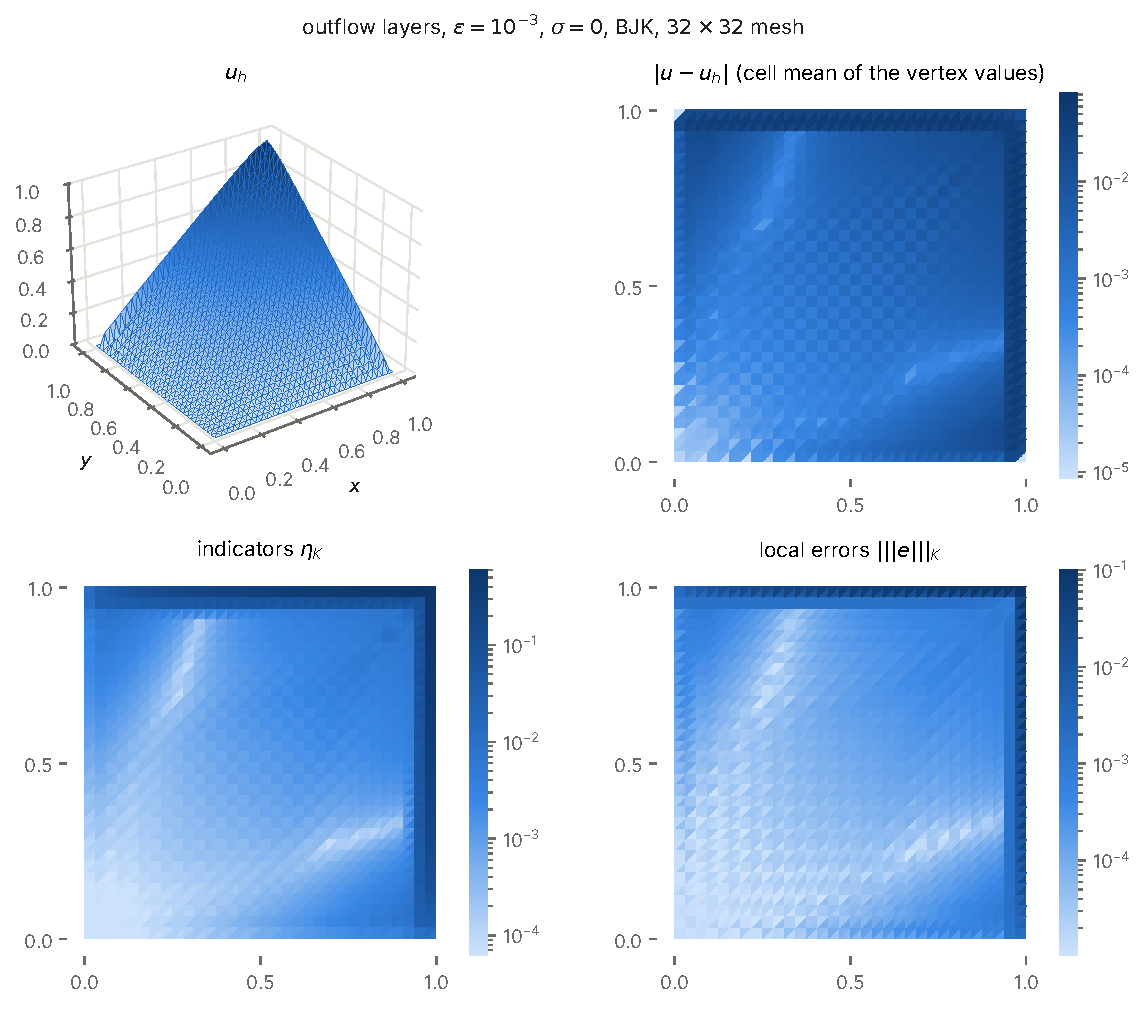
\includegraphics[width=\textwidth]{figures/sv_snap.pdf}
\caption{Layers problem, $\eps=10^{-3}$, $\sigma=0$, BJK, $n=32$: discrete solution $u_h$, indicators
$\eta_K$ and local errors $\tnorm{e}_K$ (logarithmic colour scale, common to both).}
\label{fig:snap}
\end{figure}

\subsection{Uniform refinement}\label{sec:num-conv}

Table~\ref{tab:conv} and Figure~\ref{fig:conv} report uniform refinement from $n=8$ to $n=128$.
\begin{itemize}
  \item \textbf{Smooth solution, $\eps=10^{-2}$.} $E$ and $\eta_E$ converge at the optimal rate $1$ in
  $h$ once the mesh resolves the solution; on the coarse meshes both decrease faster, because the
  stabilisation term $\|\Stil\|_*$ dominates $E$ there and decreases at a higher rate. The effectivity
  $I_E$ lies between $3.15$ and $3.29$ for $\sigma=0$ and $\sigma=1$ alike. The energy-norm index $I$
  tends to $1.1$: in the diffusion-dominated regime the energy norm and the dual norm of the
  residual coincide asymptotically.
  \item \textbf{Layers, $\eps=10^{-2}$.} The layers are resolved only from $n=64$ on, and the
  convergence of $E$ accelerates accordingly; $I_E$ stays between $2.77$ and $2.94$.
  \item \textbf{Layers, $\eps=10^{-4}$.} The meshes never resolve the layers. The energy error
  $\tnorm{e}$ \emph{increases} under refinement, because the error, concentrated in the outflow
  cells, sees an increasing part of the layer, while $E$ is dominated by the convective dual norm and
  decreases at the rate $0.45$--$0.53$; $\eta_E$ follows it with the rate $0.49$--$0.55$. The index $I_E$
  is $3.07$--$3.31$ on every mesh, whereas the energy-norm index $I$ falls from $833$ to $18.7$: the
  energy-norm bound is guaranteed but useless in this regime, which is why the error is measured in
  $E$.
\end{itemize}

\input{tables/conv}

\begin{figure}[!htbp]
\centering
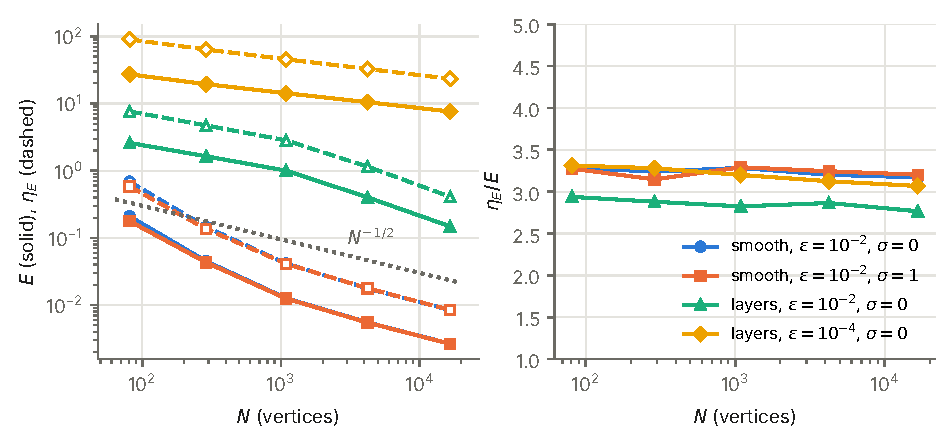
\includegraphics[width=\textwidth]{figures/sv_conv.pdf}
\caption{Uniform refinement in 2D, BJK. Left: $E$ (solid) and $\eta_E$ (dashed, open markers).
Right: effectivity index $I_E=\eta_E/E$.}
\label{fig:conv}
\end{figure}

\subsection{Robustness in \texorpdfstring{$\eps$}{eps}, \texorpdfstring{$\sigma$}{sigma} and the stabilisation}\label{sec:num-robust}

Table~\ref{tab:sweep} and Figure~\ref{fig:sweep} sweep $\eps$ from $10^{-1}$ to $10^{-8}$ on the fixed
mesh $n=32$, for $\sigma\in\{0,1\}$, both stabilisations and both problems.
\begin{itemize}
  \item \textbf{$\sigma=0$.} $I_E$ lies in $2.80$--$3.23$ for the layers problem and in $3.15$--$3.78$
  for the smooth problem, and becomes constant for $\eps\le10^{-5}$. $I_\oplus$ stays below $4.9$,
  and the stabilisation part is estimated sharply, $I_S=1.21$--$1.34$. BJK and SMUAS give the
  same indices $I_E$ and $I_\oplus$ to within $3\,\%$, as Remark~\ref{rem:robust} predicts: the limiter enters only
  through the functional, not the constants.
  \item \textbf{Energy norm.} The energy-norm index $I$ grows like $\eps^{-1}$ for $\sigma=0$, up to
  $2.5\cdot10^6$ at $\eps=10^{-8}$; the guaranteed energy-norm bound of \cite{ABR17} behaves in the
  same way. For $\sigma=1$, $I$ saturates at about $60$--$90$, the reaction giving $L^2$ control, while
  the ABR17 bound keeps growing ($1.3\cdot10^4$ at $\eps=10^{-8}$), because its reaction cut-off is not
  robust.
  \item \textbf{$\sigma=1$, small $\eps$.} Down to $\eps=10^{-6}$, $I_E$ stays in $2.7$--$3.2$ for the
  layers problem and in $3.2$--$4.9$ for the smooth one. For $\eps<10^{-6}$ it rises, to $5.5$ (layers)
  and $6.0$ (smooth) at $\eps=10^{-8}$. This increase comes from $I_S$ ($7.8$ and $10.4$ at
  $\eps=10^{-8}$), while $I_\oplus$ \emph{decreases}. This is consistent with a
  reference effect rather than with a loss of robustness: for $\sigma>0$, the Riesz representative of
  $\Stil$ has layers of width $(\eps/\sigma)^{1/2}=10^{-4}$, far below the mesh size $3\cdot10^{-2}$, so
  the same-mesh $P_2$ reference underestimates $\|\Stil\|_*$. Theorem~\ref{thm:eff} bounds $\eta_S$ by
  the true dual norm, independently of $\eps$. \adapt{The adaptive runs of Section~\ref{sec:num-unad} confirm this:
  once the mesh resolves the layers, $I_S$ falls to $1.5$--$1.6$ and $I_E$ to about $3$.} \asref{The
  asymptotic reference below makes this quantitative.}
\end{itemize}

\input{tables/sweep}

{\color{teal}
\paragraph{An asymptotically exact reference for $\|\Stil\|_*$.} For $\theta\ll1$ the dual norm of the
stabilisation functional can be evaluated without resolving its Riesz representative. With
$q=A\nabla u_h$ cellwise constant, $\Stil(v)=(q,\nabla v)=-\sum_F(\jump{q\cdot n},v)_F$ for $v\in H^1_D$, since
$\dv q=0$ in each cell. Away from the vertices, the Riesz representative is a sum of one-dimensional layers
$-\eps z''+\sigma z=\jump{q\cdot n}\,\delta_F$ across the faces, each of energy
$\jump{q\cdot n}^2/(2(\eps\sigma)^{1/2})$ per unit length. Hence
\begin{equation}\label{eq:Sasym}
  \|\Stil\|_*^2=\sum_{F\text{ interior}}\frac{\|\jump{q\cdot n}\|_F^2}{2(\eps\sigma)^{1/2}}\,\bigl(1+O(\theta)\bigr),
  \qquad \theta\to0,
\end{equation}
and the same sum over the faces interior to $\tilde\omega_K$ gives $\|\Stil\|_{*,\tilde\omega_K}^2$.
Table~\ref{tab:refref} and Figure~\ref{fig:refref} compare this value with $P_2$ references on the same mesh and on
$k$-times refined meshes ($k=2,4,8$), for the layers problem on the $16\times16$ mesh with $\sigma\in\{1,10^4\}$, using
the A+S estimator alone (without the direct variant of Remark~\ref{rem:direct}).
\begin{itemize}
  \item \textbf{The references.} At $\theta=0.11$ the asymptotic value agrees with the refined reference to $1\,\%$
  ($2.92$ against $2.95$). For smaller $\theta$ the $P_2$ references are far from converged: at $\theta=10^{-5}$ the
  same-mesh value underestimates $\|\Stil\|_*$ by a factor $85$, and even the $8$ times refined one by a factor $30$.
  \item \textbf{Theorem~\ref{thm:eff} for $\ell=-\Stil$.} Measured against \eqref{eq:Sasym}, the index
  $I_S=\eta_{-\Stil}/\|\Stil\|_*$ lies in $1.64$--$2.22$ for all $\theta\le10^{-2}$; the local ratio
  $\max_K\eta_{S,K}^2/\|\Stil\|_{*,\tilde\omega_K}^2$ lies in $0.58$--$1.56$. For this functional the theorem has no
  oscillation term, so this is a direct confirmation of robust global and local efficiency in the reaction regime.
  \item \textbf{The error measure.} With $\|\Stil\|_*$ from \eqref{eq:Sasym} and the other two parts of $E$ from the
  $8$ times refined mesh, $\eta_E/E$ stays in $8.3$--$10.2$ over three decades of $\theta$, whereas the same-mesh
  reference gives values up to $284$. The rises of $I_E$ in Table~\ref{tab:sweep} and in Section~\ref{sec:num-unad} at
  small $\theta$ are therefore an artifact of the reference, not a loss of robustness.
\end{itemize}
}

\input{tables/refref}

\begin{figure}[!htbp]
\centering
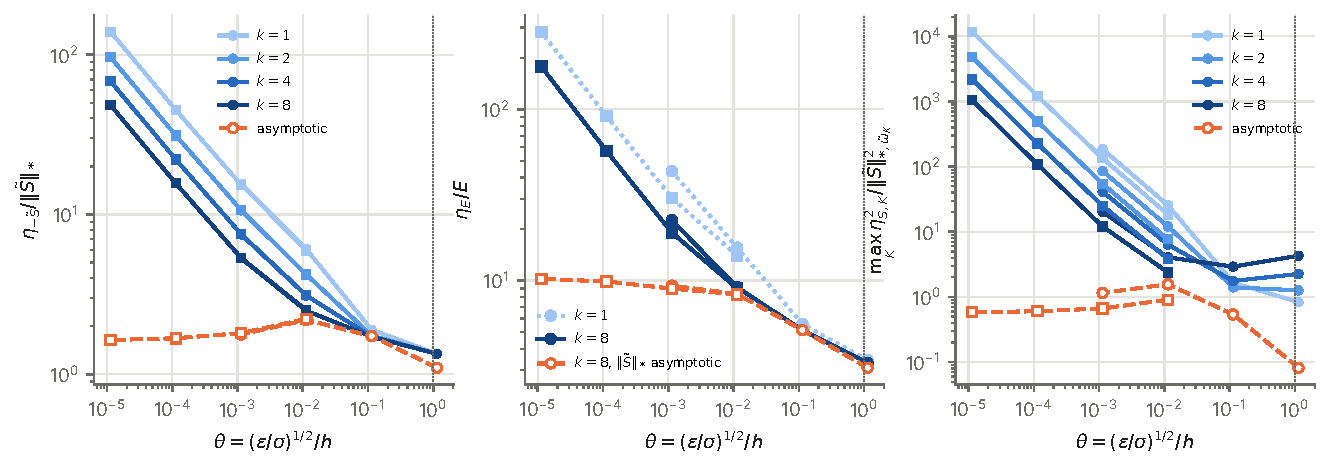
\includegraphics[width=\textwidth]{figures/sv_refref.pdf}
\caption{\asref{Reaction regime, layers problem, $n=16$, A+S estimator; circles $\sigma=1$, squares $\sigma=10^4$.
Left: $\eta_{-\Stil}/\|\Stil\|_*$ with $P_2$ references on $k$-times refined meshes and with the asymptotic value
\eqref{eq:Sasym}. Middle: $\eta_E/E$ with the same-mesh and the $8$ times refined references, and with
$\|\Stil\|_*$ from \eqref{eq:Sasym}. Right: the local ratio for $\ell=-\Stil$; the refined references are lower bounds
of the local dual norms, so these ratios are upper estimates; the asymptotic value is valid only for $\theta\ll1$.}}
\label{fig:refref}
\end{figure}

\begin{figure}[!htbp]
\centering
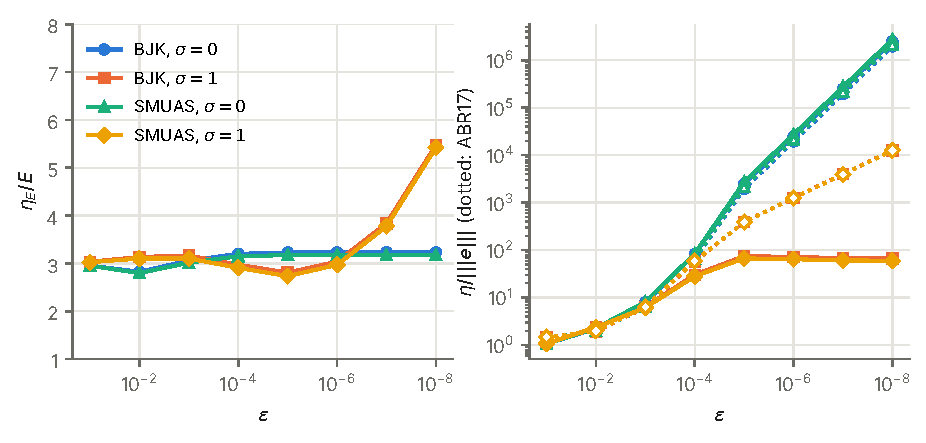
\includegraphics[width=\textwidth]{figures/sv_sweep.pdf}
\caption{Layers problem, $n=32$, as functions of $\eps$. Left: $I_E=\eta_E/E$. Right: the energy-norm
indices $\eta/\tnorm{e}$ (solid) and, dotted with open markers, that of the guaranteed bound of
\cite{ABR17}.}
\label{fig:sweep}
\end{figure}

\subsection{Variable reaction}\label{sec:num-cb}

With $c=1+(c_{\max}-1)xy$ and $\sigma=1$, the constant of (H3) is $\|c\|_\infty/\sigma=c_{\max}$, attained at
the vertex $(1,1)$. \refe{The computed $c_b$ is the sampled enclosure of Remark~\ref{rem:CF}, which is diagnostic: $c$ is not
affine on the cells, so the sampled maximum is enlarged by $\frac{h_K}2\max|\nabla c|$; here this gives} $c_b=1.12\,c_{\max}$, $1.06\,c_{\max}$
and $1.03\,c_{\max}$ for $n=8,16,32$, and $\kappa=2+c_b$ (Table~\ref{tab:cb}). The bound $E\le\eta_E$ holds in
all runs. The index of $\eta_{E,c}$ grows at most linearly, $\eta_{E,c}/E_c\le3\,c_b$ in all runs, as
Corollary~\ref{cor:twoc} predicts; it is often much smaller, down to $0.05\,c_b$, because the factor $M=c_b$ in front of $\tnorm{e}$ in $E_c$ also enlarges the
error measure. The index of $\eta_E$ grows faster, up to $5.2\,c_b$ at $c_b\approx10^3$, but stays far
below the worst case $(1+c_b)^2$ of Corollary~\ref{cor:two}. A variable reaction with a small lower
bound $\sigma$ is therefore the one situation in which the estimator loses its robustness, in
accordance with the theory; Section~\ref{sec:concl} discusses how to remove it.

\input{tables/cb}

\subsection{Local efficiency}\label{sec:num-loc}

Table~\ref{tab:loc} reports the localised measure for the layers problem on the $16\times16$ mesh. The
local ratio $\max_K\eta_K^2/E_{\mathrm{loc}}(\tilde\omega_K)^2$ is at most $0.51$ in all cases, and
independent of $\eps$ for $\eps\le10^{-4}$: the estimator is locally efficient, as stated in
Theorem~\ref{thm:loc}. The ratio $E_{\mathrm{loc}}/E$ lies between $0.48$ and $1.01$, so on these
problems the localised measure captures most of the global one, and the guaranteed bound
$E_{\mathrm{loc}}\le\sqrt{d+1}\,\eta_E$ of Theorem~\ref{thm:loc} overestimates $E_{\mathrm{loc}}$ by a
factor $5$--$12$. The largest value, $\eta_E/E_{\mathrm{loc}}=7.0$ for $\sigma=1$ and $\eps=10^{-8}$, is the
same reference effect as in Section~\ref{sec:num-robust}.

\input{tables/loc}

\subsection{Adaptive refinement}\label{sec:num-adapt}

Starting from the $8\times8$ mesh, we mark by the indicators $\eta_K=\eta_{A,K}+\eta_{S,K}$ with the
dual strategy of \cite{AJ27} (all cells with $\eta_K\ge\theta\max\eta$, $\theta=0.5$, reduced until at least
$5\,\%$ of the cells are marked) and refine by red--green refinement, until $N>3\cdot10^4$.
Table~\ref{tab:adapt} and Figures~\ref{fig:adapt} and~\ref{fig:adaptmesh} show the results for the layers
problem.
\begin{itemize}
  \item \textbf{Effectivity.} $I_E$ stays between $2.86$ and $3.55$ in every loop of all three runs, from
  $N=81$ to $N=45\,094$, while the local mesh size spans three orders of magnitude.
  \item \textbf{Where the mesh is refined.} The refinement concentrates in the outflow layers at $x=1$ and
  $y=1$ (Figure~\ref{fig:adaptmesh}); the smallest cells have $h_{\min}=3.5\cdot10^{-4}$ for $\eps=10^{-3}$,
  below $\eps$, so the layers are resolved, and $h_{\min}=1.7\cdot10^{-4}$ for $\eps=10^{-5}$, where they are not.
  \item \textbf{Convergence.} For $\eps=10^{-3}$, $E$ decreases at the rate $1.8$--$1.9$ with respect to
  $N^{-1/2}$ over the second half of the loops: this is the pre-asymptotic phase in which the layers become
  resolved, faster than the optimal rate $1$. For $\eps=10^{-5}$ the rate is $0.98$. On the finest uniform mesh
  ($N=16\,641$) the error $E$ is $18$, $4.4$ and $17$ times larger than the adaptive error at the same $N$.
  Under uniform refinement $E$ decreases at the rate $0.46$--$0.60$ for $\sigma=0$ and $0.04$--$0.51$ for
  $\sigma=1$, because the layers are never resolved; the index $I_E$ is $2.86$--$3.37$ there as well.
  \item \textbf{Energy norm.} Along the adaptive runs the energy-norm index $I$ falls from $29$ to $1.1$
  ($\eps=10^{-3}$) and from $8.4\cdot10^3$ to $6.2$ ($\eps=10^{-5}$): once the mesh resolves the layers, the
  energy error and the dual norm of the residual become comparable, while $I_E$ is insensitive to this.
\end{itemize}

\input{tables/adapt}

\begin{figure}[!htbp]
\centering
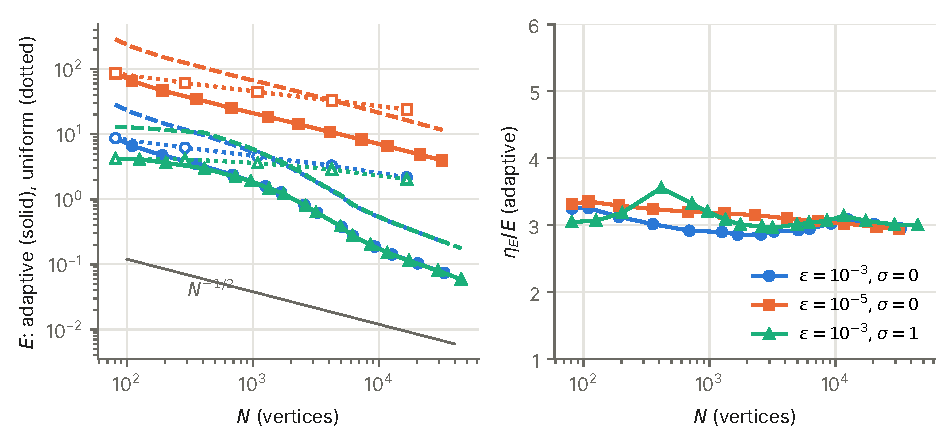
\includegraphics[width=\textwidth]{figures/sv_adapt.pdf}
\caption{Adaptive refinement, layers problem, BJK. Left: $E$ for adaptive (solid) and uniform (dotted, open
markers) refinement, and $\eta_E$ for the adaptive runs (dashed). Right: $I_E$ along the adaptive runs.}
\label{fig:adapt}
\end{figure}

\begin{figure}[!htbp]
\centering
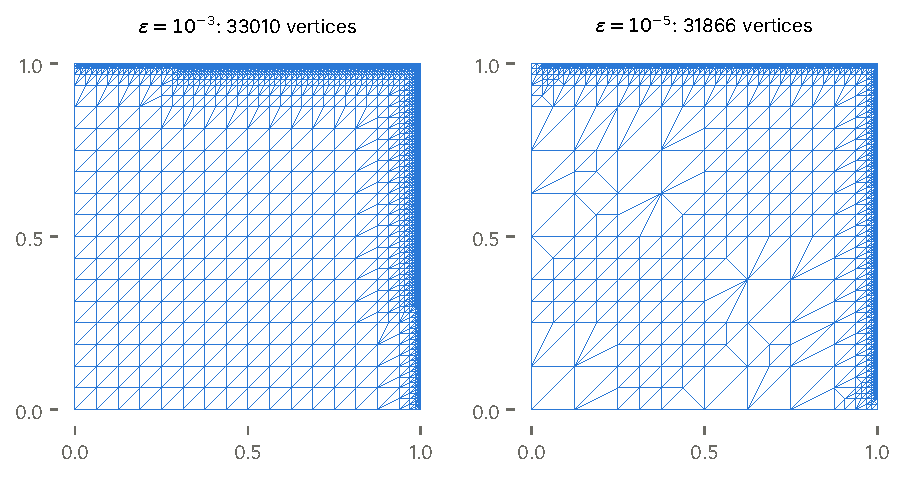
\includegraphics[width=\textwidth]{figures/sv_adapt_mesh.pdf}
\caption{Final adaptive meshes, layers problem, $\sigma=0$.}
\label{fig:adaptmesh}
\end{figure}

\subsection{\adapt{Uniform versus adaptive refinement}}\label{sec:num-unad}
{\color{magenta}

We repeat the uniform-mesh studies of Tables~\ref{tab:conv} and~\ref{tab:sweep} with adaptive refinement:
the same problems, the same marking as in Section~\ref{sec:num-adapt}, from the $8\times8$ mesh up to
$N\approx2\cdot10^4$ (Table~\ref{tab:conv}) and $N\approx10^4$ (Table~\ref{tab:sweep}). For the robustness
sweep we compare at equal cost: the adaptive loop whose $N$ is closest to $N=1089$, the size of the $32\times32$
mesh of Table~\ref{tab:sweep}.

\paragraph{Refinement studies (Figure~\ref{fig:aconv}).}
\begin{itemize}
  \item \textbf{Effectivity.} Along the adaptive runs $I_E$ lies in $2.83$--$4.18$ and tends to the same values
  as on uniform meshes, about $3.0$--$3.2$. The bound held in every loop.
  \item \textbf{Accuracy.} For the smooth solution, adaptive refinement gains nothing: at $N=16\,641$ the two
  errors agree to within $1\,\%$, and $E$ converges at the rate $1$ in both cases. For the layers problem the
  uniform error is $5.4$ ($\eps=10^{-2}$) and $5.9$ ($\eps=10^{-4}$) times the adaptive one at the same $N$.
  For $\eps=10^{-4}$, $E$ converges at the rate $0.47$ under uniform refinement and at $1.4$--$1.9$ in the last
  adaptive loops, in which the layers become resolved.
\end{itemize}

\begin{figure}[!htbp]
\centering
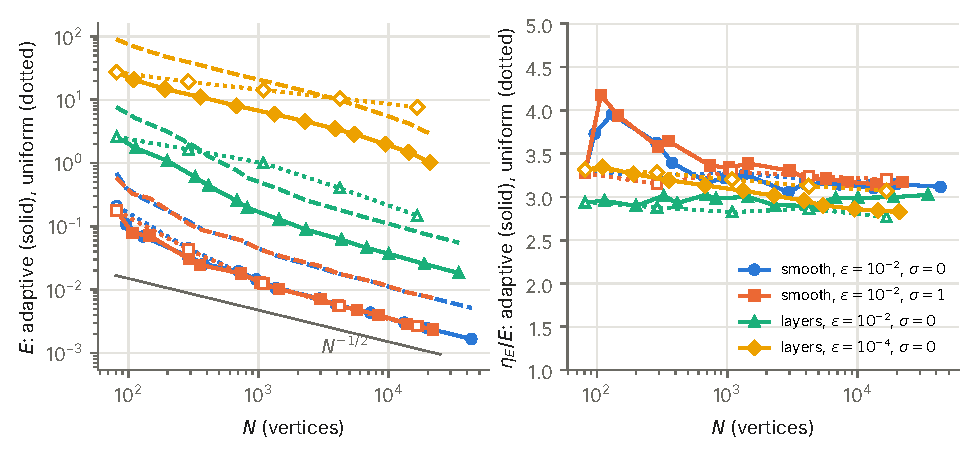
\includegraphics[width=\textwidth]{figures/sv_aconv.pdf}
\caption{\adapt{The cases of Table~\ref{tab:conv} under adaptive refinement. Left: $E$ for adaptive (solid) and uniform
(dotted, open markers) refinement, and $\eta_E$ for the adaptive runs (dashed). Right: $I_E$, adaptive (solid) and
uniform (dotted).}}
\label{fig:aconv}
\end{figure}

\paragraph{Robustness sweep (Figures~\ref{fig:abudget} and~\ref{fig:aloops}).}
\begin{itemize}
  \item \textbf{$\sigma=0$.} At equal cost, $I_E=2.89$--$3.22$ on the adaptive meshes against $2.80$--$3.23$ on the
  uniform mesh, for all $\eps$ and both stabilisations, and it stays in $2.82$--$3.35$ over all loops: the
  estimator is as robust on the meshes it generates as on the fixed mesh.
  \item \textbf{$\sigma=1$, small $\eps$.} The rise of $I_E$ to $5.4$--$5.5$ on the uniform mesh at
  $\eps\le10^{-7}$ (Section~\ref{sec:num-robust}) does not occur at equal cost on the adaptive meshes, where
  $I_E=2.75$--$3.16$. Figure~\ref{fig:aloops} shows why. The large values, up to $9.6$, appear only on the
  coarse initial mesh, and they come from the stabilisation part: $I_S=17.8$ at $N=81$ for $\eps=10^{-8}$. As the
  mesh resolves the layers, $I_S$ falls to $1.5$--$1.6$ and $I_E$ returns to about $3$. This confirms that the
  rise on the uniform mesh is a property of the under-resolved $P_2$ reference for $\|\Stil\|_*$, not of the
  estimator.
  \item \textbf{Smooth problem.} For $\eps\le10^{-3}$ the adaptive indices are higher than the uniform ones at
  equal cost: $I_E=4.0$--$5.3$ against $3.6$--$3.8$ for $\sigma=0$, and $4.5$--$6.0$ against $3.9$--$6.0$ for
  $\sigma=1$. Along the runs they reach $7.8$ after the first loop, and $10.9$ on the initial mesh. For $\sigma=1$
  and $\eps\le10^{-6}$ the fixed-point iteration reaches the iteration limit $2\cdot10^4$ on most meshes beyond
  $N\approx1100$, and the bound holds at these iterates.
  \item \textbf{Energy norm.} At $\sigma=0$ the energy-norm index still grows like $\eps^{-1}$ on the adaptive meshes,
  to $4\cdot10^5$ at $\eps=10^{-8}$ (uniform: $2.5\cdot10^6$); only the augmented measure is robust.
  \item \textbf{An open point.} For the layers problem with $\sigma=1$ and $\eps=10^{-6}$, $I_E$ rises again in the
  last loops, from $2.8$ to $4.3$, together with $I_\oplus$ (from $3.2$ to $6.6$). We have not identified the cause;
  it may be the convective part of the reference becoming resolved, and would need runs beyond $N=10^4$.
\end{itemize}

\begin{figure}[!htbp]
\centering
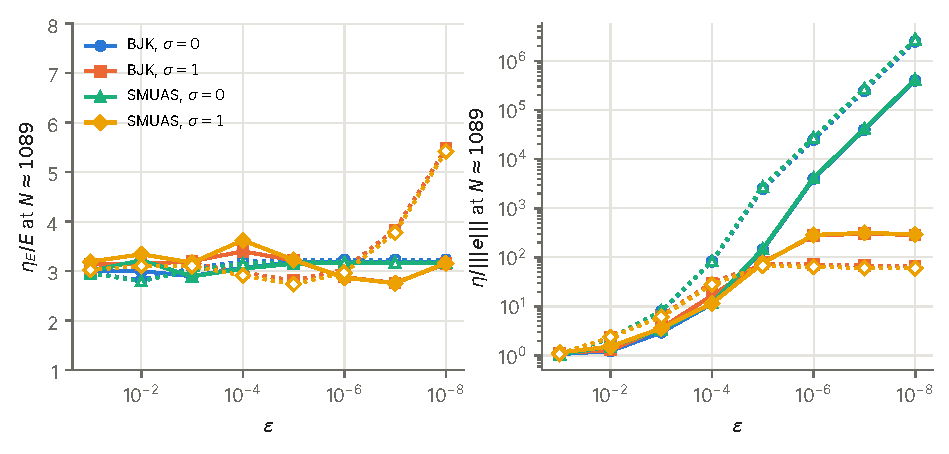
\includegraphics[width=\textwidth]{figures/sv_asweep_budget.pdf}
\caption{\adapt{The robustness sweep of Table~\ref{tab:sweep} at equal cost, layers problem: adaptive meshes with
$N\approx1089$ (solid) against the uniform $32\times32$ mesh (dotted, open markers). Left: $I_E$. Right: the
energy-norm index $\eta/\tnorm{e}$.}}
\label{fig:abudget}
\end{figure}

\begin{figure}[!htbp]
\centering
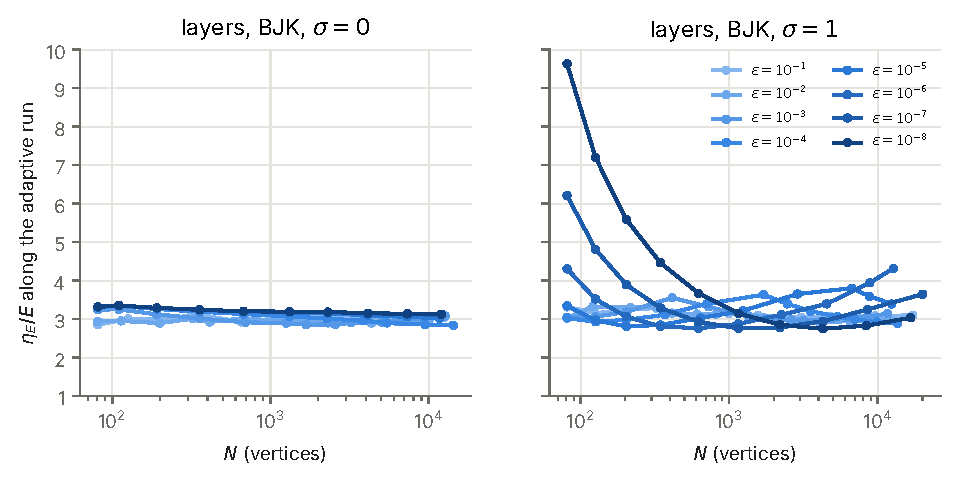
\includegraphics[width=\textwidth]{figures/sv_asweep_loops.pdf}
\caption{\adapt{$I_E$ along the adaptive runs of the robustness sweep, layers problem, BJK; one line per $\eps$, darker for
smaller $\eps$.}}
\label{fig:aloops}
\end{figure}

\paragraph{Which refinement to use.} For computing solutions, adaptive refinement is clearly preferable when the
solution has layers, by factors $4$--$18$ in $E$ at equal $N$, and it is what the estimator is designed for. For
testing the theory, the uniform meshes remain the primary evidence: a fixed coarse mesh keeps the layers
unresolved, which is the regime in which robustness can fail, isolates the dependence on $\eps$ and $\sigma$, and
is the only setting in which rates in $h$ are meaningful. The adaptive runs confirm that the effectivity stays at
about $3$ on the meshes the estimator generates itself.
}% end of the magenta block

\subsection{Inexact iterates and adaptive stopping}\label{sec:num-stop}

\paragraph{Iterates.} Table~\ref{tab:iter} and Figure~\ref{fig:iter} evaluate the estimator at the
fixed-point iterates $u^i$ on the $16\times16$ mesh. The index $I_E$ stays between $2.9$ and $5.3$ at
every iterate, including the first one, where the algebraic part $\eta_{\mathrm{alg}}$ is up to $71\,\%$
of $\eta_{\mathrm{disc}}$: this is part~2 of Proposition~\ref{prop:stop}, efficiency at every iterate
without any condition on the algebraic error. The ratio $\eta_{\mathrm{alg}}/\eta_{\mathrm{disc}}$
decreases monotonically for all problems except the smooth one with $\eps=10^{-6}$ and $\sigma=0$, for
which the fixed-point iteration does not converge in $2\cdot10^4$ iterations; there the ratio stalls
between $10^{-3}$ and $4\cdot10^{-3}$. In that case the error is smallest at $i\approx10$, $E(u^{10})=4.8$, and grows to
$8.4$ at $i=2\cdot10^4$: further iterations make the iterate worse in $E$, and the estimator, which is
efficient at every iterate, reflects this.

\input{tables/iter}

\begin{figure}[!htbp]
\centering
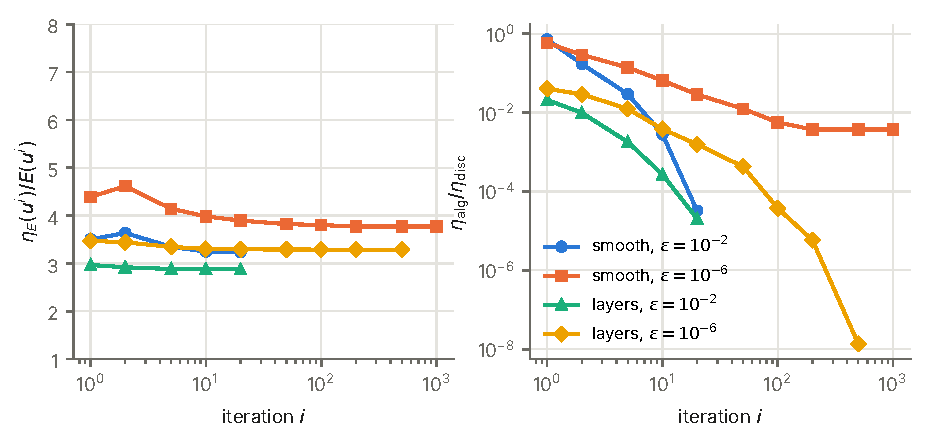
\includegraphics[width=\textwidth]{figures/sv_iter.pdf}
\caption{Fixed-point iterates, BJK, $\sigma=0$, $n=16$. Left: $I_E$ at the iterate $u^i$. Right: the
ratio $\eta_{\mathrm{alg}}/\eta_{\mathrm{disc}}$ (points with a ratio below $10^{-8}$ are omitted).}
\label{fig:iter}
\end{figure}

\paragraph{Adaptive stopping.} Table~\ref{tab:stop} runs five adaptive loops \refe{as in} Section~\ref{sec:num-adapt}
in which the fixed-point iteration is stopped either at the fixed tolerance $\|r\|\le10^{-10}\sqrt N$ or by
the criterion \eqref{eq:stop}, $\eta_{\mathrm{alg}}\le\gamma\eta_{\mathrm{disc}}$, with
$\eta_{\mathrm{disc}}=\eta_E-\eta_{\mathrm{alg}}$; each loop starts from the zero initial guess.
\begin{itemize}
  \item \textbf{Savings.} With $\gamma=0.1$, the total number of iterations drops from $227$ to $25$ (smooth,
  $\eps=10^{-2}$) and from $2323$ to $25$ (layers, $\eps=10^{-4}$), by factors $9$ and $93$; with $\gamma=0.01$
  the factors are $4.5$ and $46$.
  \item \textbf{Accuracy.} The final error $E$ changes by at most $6\,\%$ ($\gamma=0.1$, layers) and by at most
  $0.3\,\%$ for $\gamma\le0.01$. The index $I_E$ stays in $3.1$--$4.8$ in all runs, and in every stopped loop
  $\eta_{\mathrm{alg}}/\eta_{\mathrm{disc}}\le\gamma$, so $E\le(1+\gamma)\eta_{\mathrm{disc}}$
  (Proposition~\ref{prop:stop}, part~3).
  \item \textbf{Non-converging iteration.} For the smooth problem with $\eps=10^{-6}$ the fixed-point
  iteration does not reach the tolerance within $10^4$ iterations on any mesh, and $50\,000$ iterations give
  $E=3.22$. The criterion with $\gamma=0.1$ stops after $5$--$15$ iterations per loop, $50$ in total, with a
  \emph{smaller} error, $E=1.98$: as in Figure~\ref{fig:iter}, the early iterates are better than the late
  ones. For $\gamma=10^{-3}$ the criterion fires in only one of the five loops, since $\eta_{\mathrm{alg}}/\eta_{\mathrm{disc}}$ stalls
  at about $3\cdot10^{-3}$; this is a property of the iteration, not of the estimator.
\end{itemize}

\input{tables/stop}

\subsection{Variable diffusion}\label{sec:num-vareps}

Table~\ref{tab:vareps} reports the variable-diffusion problems on the meshes $n=8,16,32$. All bounds are
guaranteed. For the smooth coefficient, the oscillation $\eta_\eps$ converges at the rate $2.09$--$2.13$
in $h$, in accordance with Lemma~\ref{lem:V}(iii), and is at most $12\,\%$ of $\eta$ (at contrast $10^4$ on
the coarsest mesh). For the jump aligned with the mesh, $\Pi_1\eps=\eps$ and $\eta_\eps=0$. The
effectivity $I_E$ lies in $2.6$--$4.5$ for contrasts up to $10^4$, for $\eps=10^{-2}$ and $10^{-6}$ alike. For
the jump it does not grow with the contrast; for the smooth coefficient it grows mildly, from
$3.1$ at contrast $1$ to at most $4.3$ at contrast $10^4$ (on the coarsest mesh). This is the quasi-monotone case; the constants of
Theorem~\ref{thm:vareps} depend on the patch contrast, but for an aligned jump that contrast does not
show up in the indices. Checkerboard (non-quasi-monotone) coefficients are not tested; for them no
local estimator can be robust \cite{Li26}.

\input{tables/vareps}

\subsection{Three dimensions}\label{sec:num-3d}

Table~\ref{tab:d3} repeats the uniform-refinement study on the unit cube ($n=4,8,16$, up to $N=4913$
vertices and $24\,576$ tetrahedra).
\begin{itemize}
  \item \textbf{Layers.} $I_E=2.94$--$3.55$ for $\eps=10^{-2}$ and $10^{-6}$, as in two dimensions; $I_\oplus\le4.9$
  and $I_S=1.21$--$1.26$.
  \item \textbf{Smooth solution.} $I_E$ is higher than in two dimensions, $5.1$--$6.4$, but decreases under
  refinement for both values of $\eps$ ($5.97\to5.40$ and $6.39\to5.09$). These meshes are coarse: $E$ still
  converges at the pre-asymptotic rates $2.1$--$2.7$ in $h$, dominated by the stabilisation part
  $\|\Stil\|_*$, which is estimated sharply ($I_S=1.28$--$1.31$); the larger index comes from the convective
  dual norm on coarse tetrahedral meshes. For $\eps=10^{-6}$ on the finest mesh the fixed-point iteration does
  not converge within $2\cdot10^4$ iterations, and the bound still holds at the last iterate.
  \item \textbf{Energy norm.} As in two dimensions, $I$ is useless for $\sigma=0$ and small $\eps$
  ($1.0\cdot10^4$--$1.4\cdot10^5$ at $\eps=10^{-6}$, against $2.6$--$9.3$ at $\eps=10^{-2}$), while $I_E$ is not
  affected.
  \item \textbf{Cost.} The estimator takes about $8$\,s at $N=729$ and $220$--$240$\,s at $N=4913$ in our
  Python implementation; the cost is dominated by the vertex-patch problems in $\RTN$, whose size grows
  quickly with the number of tetrahedra per patch in three dimensions. The patch problems are independent and
  can be solved in parallel; the global $\RT_0$ defect problem takes a small fraction of the time.
\end{itemize}

\input{tables/d3}

\subsection{Summary}

The experiments answer the questions (Q1)--(Q7) as follows.
\begin{enumerate}[label=(Q\arabic*)]
  \item The bound $E\le\eta_E$ held in every run: two and three dimensions, both stabilisations,
  $\eps=10^{-1},\dots,10^{-8}$, $\sigma\in\{0,1\}$, variable reaction and diffusion, adaptive meshes and inexact
  iterates\refe{, and so did $I\ge1$, $I_\oplus\ge1$ and $I_S\ge1$. Since the references are lower bounds of the dual
  norms, this is a consistency check rather than a proof}.
  \item For constant coefficients, $I_E$ lies in $2.6$--$5.3$ in two dimensions, inexact iterates included,
  independently of $\eps$, $\sigma$, the stabilisation and the mesh; the only exception is a rise to $6.0$
  ($n=32$) and $7.1$ ($n=16$) at $\sigma=1$, $\eps\le10^{-7}$, \adapt{which the adaptive runs identify as an
  under-resolved reference for $\|\Stil\|_*$ (Section~\ref{sec:num-unad})}\asref{, as the asymptotically exact
  reference \eqref{eq:Sasym} confirms ($I_S=1.6$--$2.2$ and $\eta_E/E=8.3$--$10.2$ for $\theta$ down to $10^{-5}$)}; in three dimensions it is $2.9$--$6.4$ and
  decreases under refinement. The energy-norm index $I$, and the guaranteed bound of \cite{ABR17}, are not
  robust.
  \item The effectivity grows with $c_b$, at most linearly for $\eta_{E,c}$ and well below $c_b^2$ for $\eta_E$:
  a variable reaction with a small lower bound is the one case in which robustness is lost, as the theory
  predicts.
  \item The local ratio $\max_K\eta_K^2/E_{\mathrm{loc}}(\tilde\omega_K)^2$ is at most $0.51$.
  \item Adaptive refinement driven by $\eta_K$ resolves the layers and reduces $E$ by factors $4$--$18$
  against uniform refinement at equal $N$, with $I_E=2.9$--$3.6$ throughout. \adapt{Repeating the refinement and
  robustness studies adaptively gives the same effectivity, about $3$, as on uniform meshes.}
  \item The estimator is efficient at every iterate, and the stopping criterion saves up to $99\,\%$ of the
  iterations at a change of the error of at most $6\,\%$ ($\gamma=0.1$) or $0.3\,\%$ ($\gamma\le0.01$).
  \item For variable diffusion, $\eta_\eps$ converges at rate $2$ and $I_E$ stays in $2.6$--$4.5$ up to contrast
  $10^4$.
\end{enumerate}

\paragraph{Reproducibility.} All results are produced by the scripts \texttt{run\_numerics.py} and
\texttt{make\_figures.py} in the directory
\path{examples/convection_diffusion/sv_numerics} of \texttt{galerkit}. The first runs the experiments (about
$35$ minutes on four cores, the three-dimensional runs sequentially because of their memory use); the
second writes the tables, the figures and, for every stored solution, a VTK file
(\texttt{.vtu}) with $u_h$, $u$, $u-u_h$, $\eps$, $\eta_K$, $\tnorm{e}_K$ and the local effectivity
$\eta_K/\tnorm{e}_K$. \adapt{The figures of Section~\ref{sec:num-unad} are produced by
\texttt{make\_adaptive\_figures.py} in the same directory.}

).
% Data: examples/convection_diffusion/sv_numerics/run_numerics.py (output/*.json);
% tables and figures: make_figures.py -> tables/*.tex, figures/sv_*.{pdf,png}.
% All numbers quoted in the text below are read off those tables.

% ===========================================================================
\section{Numerical experiments}\label{sec:num}
% ===========================================================================

We test the estimator against the exact error. The questions are the ones raised by the theory:
\begin{enumerate}[label=(Q\arabic*)]
  \item Is the bound guaranteed, $E\le\eta_E$, in every run (Theorem~\ref{thm:rel})?
  \item Are the effectivity indices bounded independently of $\eps$, $\sigma$ and the stabilisation
  (Theorem~\ref{thm:eff}, Corollary~\ref{cor:two}), and do they stay bounded under refinement?
  \item Does the dependence on $c_b$ follow Corollaries~\ref{cor:two} and~\ref{cor:twoc}?
  \item Is the estimator locally efficient in the localisable measure (Theorem~\ref{thm:loc})?
  \item Do the indicators drive adaptive refinement to the optimal rate?
  \item Are the bounds valid at inexact iterates, and does the stopping criterion of
  Proposition~\ref{prop:stop} save iterations without spoiling the error?
  \item Does the variable-diffusion version keep its effectivity, with $\eta_\eps=O(h^2)$
  (Theorem~\ref{thm:vareps})?
\end{enumerate}

\subsection{Setup}

\paragraph{Discretisation.} Conforming $P_1$ elements on uniform meshes of the unit square
($n\times n$ squares, each cut into two triangles; $N=(n+1)^2$ vertices) or the unit cube ($n^3$
cubes, each cut into six tetrahedra), and on red--green refined meshes in the adaptive runs. The
stabilisations are the AFC scheme with the limiter of \cite{BJK17} (BJK), and the symmetrised
monotone upwind-type algebraic stabilisation of \cite{Kn23} (SMUAS). The nonlinear problem is solved
by the damped fixed-point iteration of \cite{AJ27} up to $\|r\|\le10^{-10}\sqrt N$, with at most
$2\cdot10^4$ iterations, unless stated otherwise.

\paragraph{Test problems} (all with $b$ constant, so $\sigma=c$, $c_b=1$ and $\kappa=3$, except in
Section~\ref{sec:num-cb}).
\begin{itemize}
  \item \emph{smooth}: $u=\prod_i\sin(\pi x_i)+x_1^2\prod_{i>1}x_i$, $b=(1,\tfrac12)$ or
  $(1,\tfrac12,\tfrac14)$, Dirichlet data on $\partial\Omega$; $f$ is computed from $u$. The solution
  has no layers, so its error is not dominated by layers, but for small $\eps$ the scheme is
  convection-dominated on every mesh used.
  \item \emph{layers}: $u=\prod_iw(x_i)$ with
  $w(s)=s-\bigl(e^{(s-1)/\eps}-e^{-1/\eps}\bigr)/\bigl(1-e^{-1/\eps}\bigr)$, $b=(1,\dots,1)$, homogeneous
  Dirichlet data; $u$ has exponential layers of width $\eps$ at the outflow boundary $x_i=1$.
  \item \emph{variable diffusion}: $u=\phi(x_1)\prod_{i>1}4x_i(1-x_i)$, either with
  $\eps(x)=\eps\,k^{x_1}$, $\phi(s)=4s(1-s)$ (\emph{smooth}), or with $\eps$ jumping from $\eps$ to $k\eps$
  at $x_1=\frac12$ and $\phi$ chosen such that the flux $\eps\phi'$ is continuous (\emph{jump}); $k$ is
  the contrast.
\end{itemize}

\paragraph{Error measures.} $\tnorm{e}$ is computed with a quadrature of degree~8. The dual norms
$\|B_A'(e,\cdot)\|_*$ and $\|\Stil\|_*$, and the local dual norms of $E_{\mathrm{loc}}$, are computed
from their Riesz representatives in the $P_2$ space on the same mesh (on each vertex patch for
$E_{\mathrm{loc}}$). These are \emph{lower} bounds of the true dual norms, so the reported effectivity
indices are slight overestimates; they become crude when the dual norm concentrates in layers that
the mesh does not resolve (see Section~\ref{sec:num-robust}). We report the effectivity indices
\[
  I=\frac{\eta}{\tnorm{e}},\qquad I_\oplus=\frac{\kappa\eta}{\tnorm{e}_\oplus},\qquad
  I_S=\frac{\eta_S}{\|\Stil\|_*},\qquad I_E=\frac{\eta_E}{E},
\]
of which $I_E$ is the one covered by Corollary~\ref{cor:two}; $I_\oplus\ge1$ and $I\ge1$ are guaranteed
too, but only $I_\oplus$ is expected to be robust.

\subsection{Solutions and indicators}

Figure~\ref{fig:snap} shows the discrete solution of the layers problem for $\eps=10^{-3}$ on the
$32\times32$ mesh, the cell indicators $\eta_K=\eta_{A,K}+\eta_{S,K}$, and the local energy errors
$\tnorm{e}_K$. The mesh does not resolve the layers ($h\approx4.4\cdot10^{-2}\gg\eps$); the AFC
solution is free of oscillations, and both the indicators and the error concentrate in the cells at
the outflow boundary, with a decay of several orders of magnitude into the interior. The indicator
is larger than $\tnorm{e}_K$ in the layer cells: it measures the residual in the dual norm, which
contains the convective part $\|B_A'(e,\cdot)\|_*$ of the error.

\begin{figure}[!htbp]
\centering
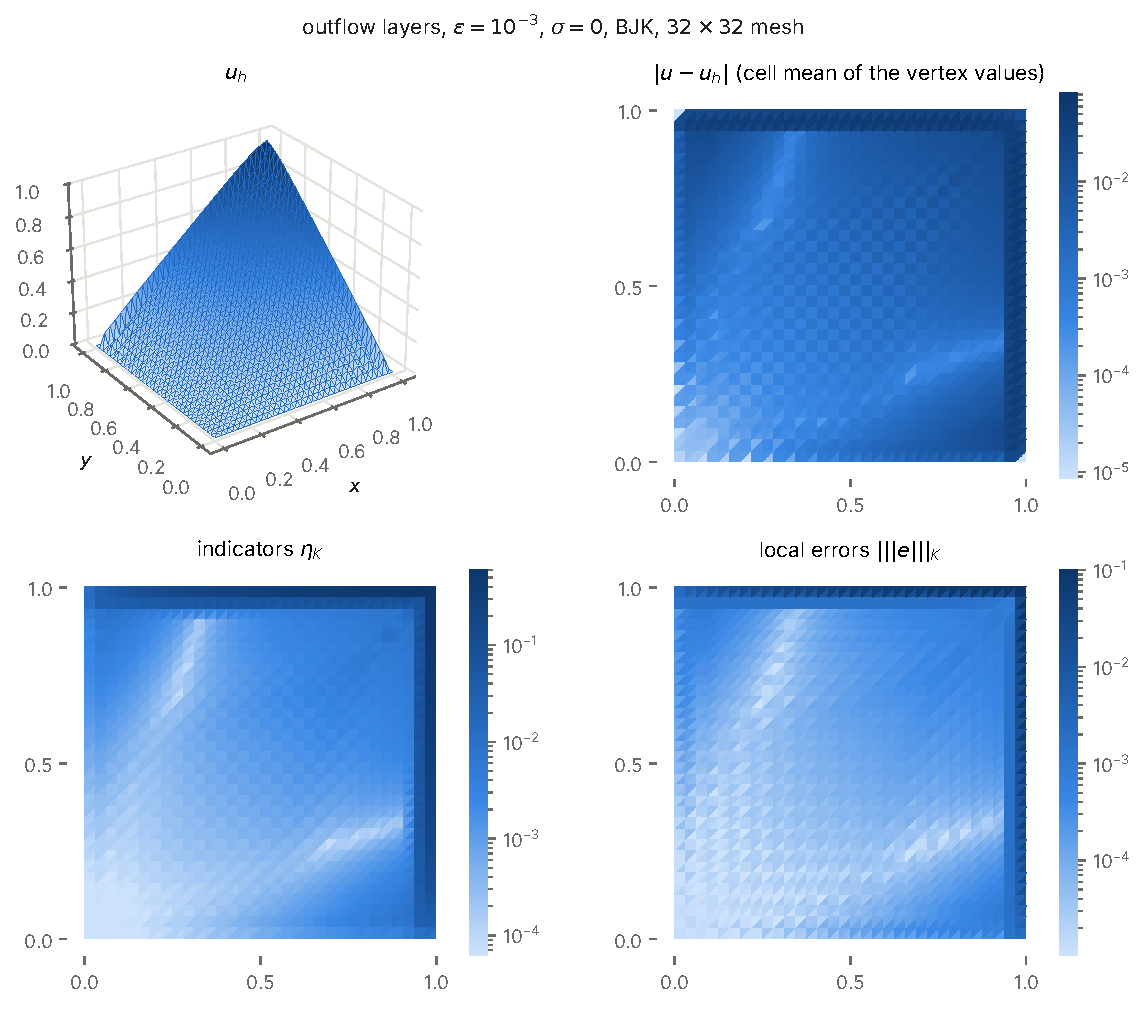
\includegraphics[width=\textwidth]{figures/sv_snap.pdf}
\caption{Layers problem, $\eps=10^{-3}$, $\sigma=0$, BJK, $n=32$: discrete solution $u_h$, indicators
$\eta_K$ and local errors $\tnorm{e}_K$ (logarithmic colour scale, common to both).}
\label{fig:snap}
\end{figure}

\subsection{Uniform refinement}\label{sec:num-conv}

Table~\ref{tab:conv} and Figure~\ref{fig:conv} report uniform refinement from $n=8$ to $n=128$.
\begin{itemize}
  \item \textbf{Smooth solution, $\eps=10^{-2}$.} $E$ and $\eta_E$ converge at the optimal rate $1$ in
  $h$ once the mesh resolves the solution; on the coarse meshes both decrease faster, because the
  stabilisation term $\|\Stil\|_*$ dominates $E$ there and decreases at a higher rate. The effectivity
  $I_E$ lies between $3.15$ and $3.29$ for $\sigma=0$ and $\sigma=1$ alike. The energy-norm index $I$
  tends to $1.1$: in the diffusion-dominated regime the energy norm and the dual norm of the
  residual coincide asymptotically.
  \item \textbf{Layers, $\eps=10^{-2}$.} The layers are resolved only from $n=64$ on, and the
  convergence of $E$ accelerates accordingly; $I_E$ stays between $2.77$ and $2.94$.
  \item \textbf{Layers, $\eps=10^{-4}$.} The meshes never resolve the layers. The energy error
  $\tnorm{e}$ \emph{increases} under refinement, because the error, concentrated in the outflow
  cells, sees an increasing part of the layer, while $E$ is dominated by the convective dual norm and
  decreases at the rate $0.45$--$0.53$; $\eta_E$ follows it with the rate $0.49$--$0.55$. The index $I_E$
  is $3.07$--$3.31$ on every mesh, whereas the energy-norm index $I$ falls from $833$ to $18.7$: the
  energy-norm bound is guaranteed but useless in this regime, which is why the error is measured in
  $E$.
\end{itemize}

% generated by examples/convection_diffusion/sv_numerics/make_figures.py; do not edit
\begin{table}[!htbp]
\centering
\small
\setlength{\tabcolsep}{4pt}
\caption{Uniform refinement in 2D, BJK. Rates with respect to $N^{-1/2}\sim h$; the expected rate is $1$ once the mesh resolves the solution. Effectivity indices $I=\eta/\tnorm{e}$, $I_\oplus=\kappa\eta/\tnorm{e}_\oplus$, $I_E=\eta_E/E$; the last column is the number of fixed-point iterations.}\label{tab:conv}
\begin{tabular}{rlllrlrrrr}
\toprule
$N$ & $\tnorm{e}$ & $E$ & rate & $\eta_E$ & rate & $I$ & $I_\oplus$ & $I_E$ & it.\\
\midrule
\multicolumn{10}{l}{\emph{smooth, $\eps=10^{-2}$, $\sigma=0$}}\\
81 & $4.88\cdot10^{-2}$ & $0.209$ &  & $0.687$ &  & 4.12 & 4.22 & 3.29 & 59\\
289 & $2.15\cdot10^{-2}$ & $4.48\cdot10^{-2}$ & 2.42 & $0.145$ & 2.45 & 2.05 & 3.86 & 3.24 & 39\\
1089 & $1.04\cdot10^{-2}$ & $1.26\cdot10^{-2}$ & 1.91 & $4.15\cdot10^{-2}$ & 1.89 & 1.31 & 3.46 & 3.28 & 18\\
4225 & $5.16\cdot10^{-3}$ & $5.51\cdot10^{-3}$ & 1.23 & $1.76\cdot10^{-2}$ & 1.26 & 1.14 & 3.24 & 3.20 & 9\\
16641 & $2.58\cdot10^{-3}$ & $2.65\cdot10^{-3}$ & 1.07 & $8.40\cdot10^{-3}$ & 1.08 & 1.09 & 3.18 & 3.17 & 6\\
\multicolumn{10}{l}{\emph{smooth, $\eps=10^{-2}$, $\sigma=1$}}\\
81 & $5.01\cdot10^{-2}$ & $0.178$ &  & $0.582$ &  & 3.34 & 4.04 & 3.27 & 56\\
289 & $2.16\cdot10^{-2}$ & $4.31\cdot10^{-2}$ & 2.23 & $0.136$ & 2.29 & 1.89 & 3.69 & 3.15 & 37\\
1089 & $1.04\cdot10^{-2}$ & $1.25\cdot10^{-2}$ & 1.87 & $4.12\cdot10^{-2}$ & 1.80 & 1.29 & 3.46 & 3.29 & 18\\
4225 & $5.16\cdot10^{-3}$ & $5.47\cdot10^{-3}$ & 1.22 & $1.77\cdot10^{-2}$ & 1.24 & 1.15 & 3.29 & 3.24 & 9\\
16641 & $2.58\cdot10^{-3}$ & $2.64\cdot10^{-3}$ & 1.06 & $8.45\cdot10^{-3}$ & 1.08 & 1.10 & 3.22 & 3.20 & 6\\
\multicolumn{10}{l}{\emph{layers, $\eps=10^{-2}$, $\sigma=0$}}\\
81 & $0.522$ & $2.6$ &  & $7.62$ &  & 4.19 & 3.78 & 2.94 & 67\\
289 & $0.471$ & $1.64$ & 0.72 & $4.72$ & 0.75 & 2.88 & 3.64 & 2.88 & 47\\
1089 & $0.366$ & $1$ & 0.74 & $2.83$ & 0.77 & 2.21 & 3.56 & 2.82 & 63\\
4225 & $0.231$ & $0.401$ & 1.35 & $1.15$ & 1.33 & 1.52 & 3.26 & 2.86 & 28\\
16641 & $0.127$ & $0.148$ & 1.46 & $0.409$ & 1.51 & 1.07 & 2.77 & 2.77 & 9\\
\multicolumn{10}{l}{\emph{layers, $\eps=10^{-4}$, $\sigma=0$}}\\
81 & $3.07\cdot10^{-2}$ & $2.72\cdot10^{1}$ &  & $9.02\cdot10^{1}$ &  & 833.01 & 4.76 & 3.31 & 405\\
289 & $6.15\cdot10^{-2}$ & $1.94\cdot10^{1}$ & 0.53 & $6.37\cdot10^{1}$ & 0.55 & 290.45 & 4.81 & 3.28 & 709\\
1089 & $0.154$ & $1.42\cdot10^{1}$ & 0.47 & $4.56\cdot10^{1}$ & 0.51 & 82.17 & 4.75 & 3.20 & 700\\
4225 & $0.242$ & $1.05\cdot10^{1}$ & 0.45 & $3.27\cdot10^{1}$ & 0.49 & 37.26 & 4.65 & 3.12 & 626\\
16641 & $0.342$ & $7.6$ & 0.47 & $2.33\cdot10^{1}$ & 0.49 & 18.72 & 4.54 & 3.07 & 566\\
\bottomrule
\end{tabular}
\end{table}


\begin{figure}[!htbp]
\centering
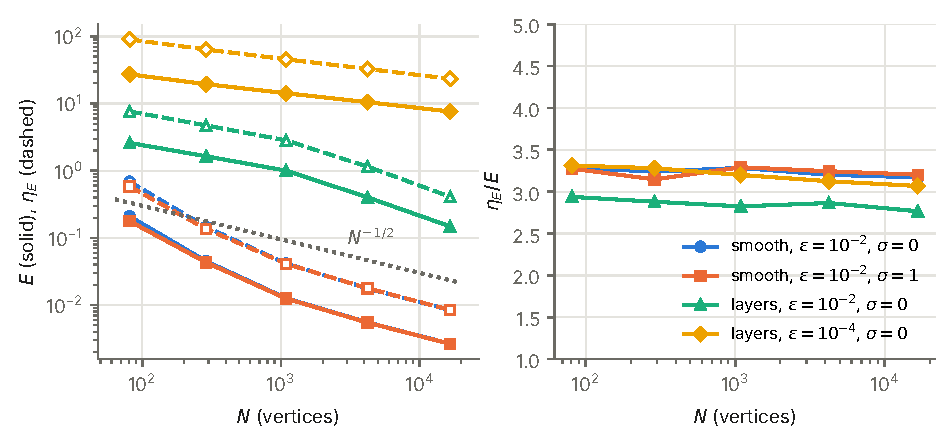
\includegraphics[width=\textwidth]{figures/sv_conv.pdf}
\caption{Uniform refinement in 2D, BJK. Left: $E$ (solid) and $\eta_E$ (dashed, open markers).
Right: effectivity index $I_E=\eta_E/E$.}
\label{fig:conv}
\end{figure}

\subsection{Robustness in \texorpdfstring{$\eps$}{eps}, \texorpdfstring{$\sigma$}{sigma} and the stabilisation}\label{sec:num-robust}

Table~\ref{tab:sweep} and Figure~\ref{fig:sweep} sweep $\eps$ from $10^{-1}$ to $10^{-8}$ on the fixed
mesh $n=32$, for $\sigma\in\{0,1\}$, both stabilisations and both problems.
\begin{itemize}
  \item \textbf{$\sigma=0$.} $I_E$ lies in $2.80$--$3.23$ for the layers problem and in $3.15$--$3.78$
  for the smooth problem, and becomes constant for $\eps\le10^{-5}$. $I_\oplus$ stays below $4.9$,
  and the stabilisation part is estimated sharply, $I_S=1.21$--$1.34$. BJK and SMUAS give the
  same indices $I_E$ and $I_\oplus$ to within $3\,\%$, as Remark~\ref{rem:robust} predicts: the limiter enters only
  through the functional, not the constants.
  \item \textbf{Energy norm.} The energy-norm index $I$ grows like $\eps^{-1}$ for $\sigma=0$, up to
  $2.5\cdot10^6$ at $\eps=10^{-8}$; the guaranteed energy-norm bound of \cite{ABR17} behaves in the
  same way. For $\sigma=1$, $I$ saturates at about $60$--$90$, the reaction giving $L^2$ control, while
  the ABR17 bound keeps growing ($1.3\cdot10^4$ at $\eps=10^{-8}$), because its reaction cut-off is not
  robust.
  \item \textbf{$\sigma=1$, small $\eps$.} Down to $\eps=10^{-6}$, $I_E$ stays in $2.7$--$3.2$ for the
  layers problem and in $3.2$--$4.9$ for the smooth one. For $\eps<10^{-6}$ it rises, to $5.5$ (layers)
  and $6.0$ (smooth) at $\eps=10^{-8}$. This increase comes from $I_S$ ($7.8$ and $10.4$ at
  $\eps=10^{-8}$), while $I_\oplus$ \emph{decreases}. This is consistent with a
  reference effect rather than with a loss of robustness: for $\sigma>0$, the Riesz representative of
  $\Stil$ has layers of width $(\eps/\sigma)^{1/2}=10^{-4}$, far below the mesh size $3\cdot10^{-2}$, so
  the same-mesh $P_2$ reference underestimates $\|\Stil\|_*$. Theorem~\ref{thm:eff} bounds $\eta_S$ by
  the true dual norm, independently of $\eps$. \adapt{The adaptive runs of Section~\ref{sec:num-unad} confirm this:
  once the mesh resolves the layers, $I_S$ falls to $1.5$--$1.6$ and $I_E$ to about $3$.} \asref{The
  asymptotic reference below makes this quantitative.}
\end{itemize}

% generated by examples/convection_diffusion/sv_numerics/make_figures.py; do not edit
\begin{table}[!htbp]
\centering
\footnotesize
\setlength{\tabcolsep}{4pt}
\caption{Robustness in $\eps$ and $\sigma$ on the uniform mesh with $n=32$ ($N=1089$). $I_E=\eta_E/E$, $I_\oplus=\kappa\eta/\tnorm{e}_\oplus$, $I_S=\eta_S/\|\Stil\|_*$, $I=\eta/\tnorm{e}$ and, for comparison, the effectivity $I_{\mathrm{ABR17}}$ of the guaranteed energy-norm bound of \cite{ABR17}.}\label{tab:sweep}
\begin{tabular}{llrrrrrrrr}
\toprule
case & index & $10^{-1}$ & $10^{-2}$ & $10^{-3}$ & $10^{-4}$ & $10^{-5}$ & $10^{-6}$ & $10^{-7}$ & $10^{-8}$\\
\midrule
layers, BJK, $\sigma=0$ & $I_E$ & 2.96 & 2.82 & 3.06 & 3.20 & 3.23 & 3.23 & 3.23 & 3.23\\
 & $I_\oplus$ & 2.98 & 3.56 & 4.30 & 4.75 & 4.84 & 4.84 & 4.84 & 4.84\\
 & $I_S$ & 1.26 & 1.24 & 1.24 & 1.22 & 1.22 & 1.22 & 1.22 & 1.22\\
 & $I$ & 1.06 & 2.21 & 7.95 & 82.17 & $2.5\cdot10^{3}$ & $2.5\cdot10^{4}$ & $2.5\cdot10^{5}$ & $2.5\cdot10^{6}$\\
 & $I_{\mathrm{ABR17}}$ & 1.47 & 1.93 & 6.26 & 64.53 & $1.9\cdot10^{3}$ & $1.9\cdot10^{4}$ & $1.9\cdot10^{5}$ & $1.9\cdot10^{6}$\\
\addlinespace
layers, BJK, $\sigma=1$ & $I_E$ & 3.03 & 3.13 & 3.16 & 2.97 & 2.81 & 3.04 & 3.83 & 5.47\\
 & $I_\oplus$ & 3.05 & 3.95 & 4.25 & 4.02 & 3.83 & 3.50 & 3.28 & 3.24\\
 & $I_S$ & 1.29 & 1.29 & 1.41 & 1.54 & 1.66 & 2.55 & 4.41 & 7.79\\
 & $I$ & 1.09 & 2.33 & 6.39 & 30.27 & 74.58 & 71.78 & 67.57 & 66.77\\
 & $I_{\mathrm{ABR17}}$ & 1.47 & 1.94 & 6.25 & 57.80 & 391.31 & $1.3\cdot10^{3}$ & $4.0\cdot10^{3}$ & $1.3\cdot10^{4}$\\
\addlinespace
layers, SMUAS, $\sigma=0$ & $I_E$ & 2.95 & 2.80 & 3.01 & 3.15 & 3.17 & 3.18 & 3.18 & 3.18\\
 & $I_\oplus$ & 2.97 & 3.57 & 4.29 & 4.73 & 4.82 & 4.82 & 4.82 & 4.82\\
 & $I_S$ & 1.34 & 1.24 & 1.25 & 1.23 & 1.23 & 1.23 & 1.23 & 1.23\\
 & $I$ & 1.06 & 2.26 & 8.09 & 83.92 & $2.7\cdot10^{3}$ & $2.7\cdot10^{4}$ & $2.7\cdot10^{5}$ & $2.7\cdot10^{6}$\\
 & $I_{\mathrm{ABR17}}$ & 1.47 & 1.97 & 6.38 & 65.99 & $2.2\cdot10^{3}$ & $2.2\cdot10^{4}$ & $2.2\cdot10^{5}$ & $2.2\cdot10^{6}$\\
\addlinespace
layers, SMUAS, $\sigma=1$ & $I_E$ & 3.03 & 3.10 & 3.10 & 2.91 & 2.73 & 2.97 & 3.78 & 5.42\\
 & $I_\oplus$ & 3.04 & 3.95 & 4.20 & 4.00 & 3.81 & 3.49 & 3.27 & 3.24\\
 & $I_S$ & 1.37 & 1.28 & 1.41 & 1.50 & 1.61 & 2.46 & 4.26 & 7.53\\
 & $I$ & 1.08 & 2.36 & 6.14 & 28.08 & 66.99 & 64.21 & 60.54 & 59.85\\
 & $I_{\mathrm{ABR17}}$ & 1.47 & 1.99 & 6.38 & 58.84 & 389.93 & $1.3\cdot10^{3}$ & $4.0\cdot10^{3}$ & $1.3\cdot10^{4}$\\
\addlinespace
smooth, BJK, $\sigma=0$ & $I_E$ & 3.15 & 3.28 & 3.76 & 3.78 & 3.58 & 3.58 & 3.58 & 3.58\\
 & $I_\oplus$ & 3.17 & 3.46 & 4.85 & 4.49 & 3.87 & 3.86 & 3.85 & 3.85\\
 & $I_S$ & 1.29 & 1.30 & 1.24 & 1.21 & 1.22 & 1.22 & 1.22 & 1.22\\
 & $I$ & 1.12 & 1.31 & 6.28 & 77.92 & 778.23 & $6.9\cdot10^{3}$ & $6.8\cdot10^{4}$ & $6.8\cdot10^{5}$\\
 & $I_{\mathrm{ABR17}}$ & 1.70 & 1.76 & 5.18 & 74.26 & 842.71 & $7.5\cdot10^{3}$ & $7.4\cdot10^{4}$ & $7.4\cdot10^{5}$\\
\addlinespace
smooth, BJK, $\sigma=1$ & $I_E$ & 3.22 & 3.29 & 3.86 & 4.66 & 4.93 & 4.81 & 5.04 & 6.00\\
 & $I_\oplus$ & 3.24 & 3.46 & 4.82 & 5.50 & 5.68 & 5.22 & 4.79 & 4.69\\
 & $I_S$ & 1.32 & 1.37 & 1.45 & 1.66 & 2.24 & 3.41 & 5.88 & 10.39\\
 & $I$ & 1.14 & 1.29 & 5.60 & 42.08 & 90.00 & 92.63 & 85.82 & 84.22\\
 & $I_{\mathrm{ABR17}}$ & 1.70 & 1.76 & 5.05 & 49.08 & 229.66 & 763.28 & $2.4\cdot10^{3}$ & $7.7\cdot10^{3}$\\
\bottomrule
\end{tabular}
\end{table}


{\color{teal}
\paragraph{An asymptotically exact reference for $\|\Stil\|_*$.} For $\theta\ll1$ the dual norm of the
stabilisation functional can be evaluated without resolving its Riesz representative. With
$q=A\nabla u_h$ cellwise constant, $\Stil(v)=(q,\nabla v)=-\sum_F(\jump{q\cdot n},v)_F$ for $v\in H^1_D$, since
$\dv q=0$ in each cell. Away from the vertices, the Riesz representative is a sum of one-dimensional layers
$-\eps z''+\sigma z=\jump{q\cdot n}\,\delta_F$ across the faces, each of energy
$\jump{q\cdot n}^2/(2(\eps\sigma)^{1/2})$ per unit length. Hence
\begin{equation}\label{eq:Sasym}
  \|\Stil\|_*^2=\sum_{F\text{ interior}}\frac{\|\jump{q\cdot n}\|_F^2}{2(\eps\sigma)^{1/2}}\,\bigl(1+O(\theta)\bigr),
  \qquad \theta\to0,
\end{equation}
and the same sum over the faces interior to $\tilde\omega_K$ gives $\|\Stil\|_{*,\tilde\omega_K}^2$.
Table~\ref{tab:refref} and Figure~\ref{fig:refref} compare this value with $P_2$ references on the same mesh and on
$k$-times refined meshes ($k=2,4,8$), for the layers problem on the $16\times16$ mesh with $\sigma\in\{1,10^4\}$, using
the A+S estimator alone (without the direct variant of Remark~\ref{rem:direct}).
\begin{itemize}
  \item \textbf{The references.} At $\theta=0.11$ the asymptotic value agrees with the refined reference to $1\,\%$
  ($2.92$ against $2.95$). For smaller $\theta$ the $P_2$ references are far from converged: at $\theta=10^{-5}$ the
  same-mesh value underestimates $\|\Stil\|_*$ by a factor $85$, and even the $8$ times refined one by a factor $30$.
  \item \textbf{Theorem~\ref{thm:eff} for $\ell=-\Stil$.} Measured against \eqref{eq:Sasym}, the index
  $I_S=\eta_{-\Stil}/\|\Stil\|_*$ lies in $1.64$--$2.22$ for all $\theta\le10^{-2}$; the local ratio
  $\max_K\eta_{S,K}^2/\|\Stil\|_{*,\tilde\omega_K}^2$ lies in $0.58$--$1.56$. For this functional the theorem has no
  oscillation term, so this is a direct confirmation of robust global and local efficiency in the reaction regime.
  \item \textbf{The error measure.} With $\|\Stil\|_*$ from \eqref{eq:Sasym} and the other two parts of $E$ from the
  $8$ times refined mesh, $\eta_E/E$ stays in $8.3$--$10.2$ over three decades of $\theta$, whereas the same-mesh
  reference gives values up to $284$. The rises of $I_E$ in Table~\ref{tab:sweep} and in Section~\ref{sec:num-unad} at
  small $\theta$ are therefore an artifact of the reference, not a loss of robustness.
\end{itemize}
}

% generated by examples/convection_diffusion/sv_numerics/make_exp36_figures.py; do not edit
\begin{table}[!htbp]
\centering
\small
\setlength{\tabcolsep}{3.5pt}
\caption{\asref{Reaction regime, layers problem, $n=16$, BJK, the A+S estimator alone. $\|\tilde S\|_*$ from $P_2$ on the same mesh ($k=1$), on the $8$ times refined mesh ($k=8$), and the asymptotic value \eqref{eq:Sasym}; $I_S=\eta_{-\tilde S}/\|\tilde S\|_*$; $\eta_E/E$ with the same-mesh reference and with $E^*$, in which $\|\tilde S\|_*$ is the larger of the $k=8$ and the asymptotic value.}}\label{tab:refref}
\begin{tabular}{rrrrrrrrrr}
\toprule
$\sigma$ & $\eps$ & $\theta$ & \multicolumn{3}{c}{$\|\tilde S\|_*$} & \multicolumn{2}{c}{$I_S$} & \multicolumn{2}{c}{$\eta_E/E$}\\
 & & & $k=1$ & $k=8$ & asympt. & $k=8$ & asympt. & $k=1$ & $E^*$\\
\midrule
1 & $10^{-2}$ & $1.1$ & 0.461 & 0.461 & 0.564 & 1.34 & 1.10 & 3.4 & 3.1 \\
1 & $10^{-4}$ & $1.1\cdot10^{-1}$ & 2.67 & 2.95 & 2.92 & 1.72 & 1.73 & 5.6 & 5.1 \\
1 & $10^{-6}$ & $1.1\cdot10^{-2}$ & 3.34 & 8.14 & 9.28 & 2.49 & 2.19 & 15.6 & 8.4 \\
1 & $10^{-8}$ & $1.1\cdot10^{-3}$ & 3.35 & 9.77 & 29.4 & 5.33 & 1.77 & 43.5 & 9.3 \\
10000 & $10^{-2}$ & $1.1\cdot10^{-2}$ & 5.02 & 11.9 & 13.5 & 2.52 & 2.22 & 14.0 & 8.3 \\
10000 & $10^{-4}$ & $1.1\cdot10^{-3}$ & 5.29 & 15.2 & 45 & 5.36 & 1.81 & 30.4 & 9.0 \\
10000 & $10^{-6}$ & $1.1\cdot10^{-4}$ & 5.29 & 15.2 & 142 & 15.68 & 1.68 & 91.1 & 9.9 \\
10000 & $10^{-8}$ & $1.1\cdot10^{-5}$ & 5.29 & 15.2 & 450 & 48.39 & 1.64 & 283.6 & 10.2 \\
\bottomrule
\end{tabular}
\end{table}


\begin{figure}[!htbp]
\centering
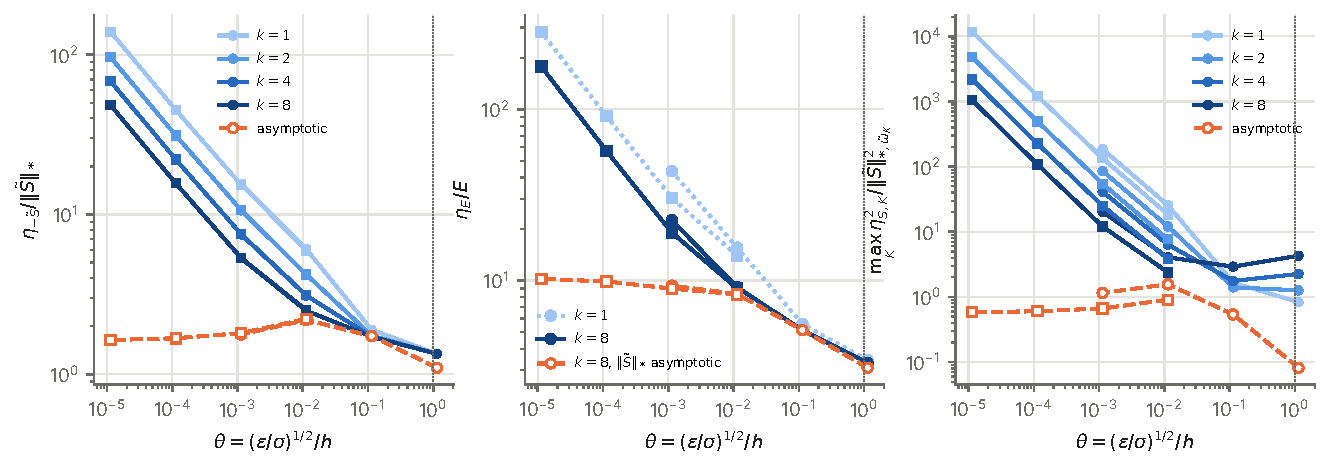
\includegraphics[width=\textwidth]{figures/sv_refref.pdf}
\caption{\asref{Reaction regime, layers problem, $n=16$, A+S estimator; circles $\sigma=1$, squares $\sigma=10^4$.
Left: $\eta_{-\Stil}/\|\Stil\|_*$ with $P_2$ references on $k$-times refined meshes and with the asymptotic value
\eqref{eq:Sasym}. Middle: $\eta_E/E$ with the same-mesh and the $8$ times refined references, and with
$\|\Stil\|_*$ from \eqref{eq:Sasym}. Right: the local ratio for $\ell=-\Stil$; the refined references are lower bounds
of the local dual norms, so these ratios are upper estimates; the asymptotic value is valid only for $\theta\ll1$.}}
\label{fig:refref}
\end{figure}

\begin{figure}[!htbp]
\centering
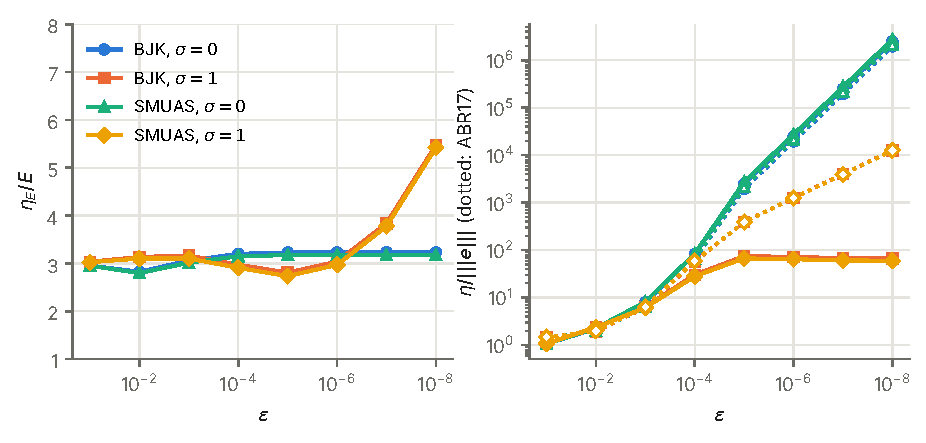
\includegraphics[width=\textwidth]{figures/sv_sweep.pdf}
\caption{Layers problem, $n=32$, as functions of $\eps$. Left: $I_E=\eta_E/E$. Right: the energy-norm
indices $\eta/\tnorm{e}$ (solid) and, dotted with open markers, that of the guaranteed bound of
\cite{ABR17}.}
\label{fig:sweep}
\end{figure}

\subsection{Variable reaction}\label{sec:num-cb}

With $c=1+(c_{\max}-1)xy$ and $\sigma=1$, the constant of (H3) is $\|c\|_\infty/\sigma=c_{\max}$, attained at
the vertex $(1,1)$. \refe{The computed $c_b$ is the sampled enclosure of Remark~\ref{rem:CF}, which is diagnostic: $c$ is not
affine on the cells, so the sampled maximum is enlarged by $\frac{h_K}2\max|\nabla c|$; here this gives} $c_b=1.12\,c_{\max}$, $1.06\,c_{\max}$
and $1.03\,c_{\max}$ for $n=8,16,32$, and $\kappa=2+c_b$ (Table~\ref{tab:cb}). The bound $E\le\eta_E$ holds in
all runs. The index of $\eta_{E,c}$ grows at most linearly, $\eta_{E,c}/E_c\le3\,c_b$ in all runs, as
Corollary~\ref{cor:twoc} predicts; it is often much smaller, down to $0.05\,c_b$, because the factor $M=c_b$ in front of $\tnorm{e}$ in $E_c$ also enlarges the
error measure. The index of $\eta_E$ grows faster, up to $5.2\,c_b$ at $c_b\approx10^3$, but stays far
below the worst case $(1+c_b)^2$ of Corollary~\ref{cor:two}. A variable reaction with a small lower
bound $\sigma$ is therefore the one situation in which the estimator loses its robustness, in
accordance with the theory; Section~\ref{sec:concl} discusses how to remove it.

% generated by examples/convection_diffusion/sv_numerics/make_figures.py; do not edit
\begin{table}[!htbp]
\centering
\small
\setlength{\tabcolsep}{4pt}
\caption{Variable reaction $c=1+(c_{\max}-1)xy$, $\sigma=1$, $\eps\in\{10^{-3},10^{-6}\}$, $n\in\{8,16,32\}$: ranges over the six runs; $c_b$ and $\kappa$ are the means of the sampled enclosures (Remark~\ref{rem:CF}; diagnostic), which exceed $c_{\max}$ by $3$--$12\,\%$.}\label{tab:cb}
\begin{tabular}{rrrllll}
\toprule
$c_{\max}$ & $c_b$ & $\kappa$ & $\eta_E/E$ & $\eta_{E,c}/E_c$ & $\eta_{E,c}/(c_bE_c)$ & $E\le\eta_E$\\
\midrule
1 & 1.00 & 3.00 & 3.85--5.34 & 3.85--5.34 & 3.85--5.34 & yes\\
10 & 10.66 & 12.66 & 14.63--19.94 & 8.69--30.35 & 0.85--2.95 & yes\\
100 & 107.22 & 109.22 & 128--271 & 12.27--216 & 0.12--2.09 & yes\\
1000 & $1.1\cdot10^{3}$ & $1.1\cdot10^{3}$ & 1618--5312 & 56.23--1125 & 0.05--1.09 & yes\\
\bottomrule
\end{tabular}
\end{table}


\subsection{Local efficiency}\label{sec:num-loc}

Table~\ref{tab:loc} reports the localised measure for the layers problem on the $16\times16$ mesh. The
local ratio $\max_K\eta_K^2/E_{\mathrm{loc}}(\tilde\omega_K)^2$ is at most $0.51$ in all cases, and
independent of $\eps$ for $\eps\le10^{-4}$: the estimator is locally efficient, as stated in
Theorem~\ref{thm:loc}. The ratio $E_{\mathrm{loc}}/E$ lies between $0.48$ and $1.01$, so on these
problems the localised measure captures most of the global one, and the guaranteed bound
$E_{\mathrm{loc}}\le\sqrt{d+1}\,\eta_E$ of Theorem~\ref{thm:loc} overestimates $E_{\mathrm{loc}}$ by a
factor $5$--$12$. The largest value, $\eta_E/E_{\mathrm{loc}}=7.0$ for $\sigma=1$ and $\eps=10^{-8}$, is the
same reference effect as in Section~\ref{sec:num-robust}.

% generated by examples/convection_diffusion/sv_numerics/make_figures.py; do not edit
\begin{table}[!htbp]
\centering
\small
\setlength{\tabcolsep}{4pt}
\caption{Localised measure (Theorem~\ref{thm:loc}), outflow layers, BJK, $n=16$. The last but one column is $\max_K\eta_K^2/E_{\mathrm{loc}}(\tilde\omega_K)^2$ with $\eta_K=\eta_{A,K}+\eta_{S,K}$.}\label{tab:loc}
\begin{tabular}{rrrrrrr}
\toprule
$\sigma$ & $\eps$ & $E_{\mathrm{loc}}/E$ & $\eta_E/E_{\mathrm{loc}}$ & $\sqrt{d+1}\,\eta_E/E_{\mathrm{loc}}$ & local max & $I_E$\\
\midrule
0 & $10^{-2}$ & 0.48 & 5.94 & 10.29 & 0.26 & 2.88\\
0 & $10^{-4}$ & 0.60 & 5.50 & 9.53 & 0.37 & 3.28\\
0 & $10^{-6}$ & 0.60 & 5.50 & 9.52 & 0.37 & 3.29\\
0 & $10^{-8}$ & 0.60 & 5.50 & 9.52 & 0.37 & 3.29\\
1 & $10^{-2}$ & 0.52 & 6.38 & 11.05 & 0.51 & 3.33\\
1 & $10^{-4}$ & 0.95 & 3.07 & 5.32 & 0.13 & 2.93\\
1 & $10^{-6}$ & 1.01 & 3.47 & 6.01 & 0.07 & 3.51\\
1 & $10^{-8}$ & 1.01 & 7.04 & 12.20 & 0.07 & 7.13\\
\bottomrule
\end{tabular}
\end{table}


\subsection{Adaptive refinement}\label{sec:num-adapt}

Starting from the $8\times8$ mesh, we mark by the indicators $\eta_K=\eta_{A,K}+\eta_{S,K}$ with the
dual strategy of \cite{AJ27} (all cells with $\eta_K\ge\theta\max\eta$, $\theta=0.5$, reduced until at least
$5\,\%$ of the cells are marked) and refine by red--green refinement, until $N>3\cdot10^4$.
Table~\ref{tab:adapt} and Figures~\ref{fig:adapt} and~\ref{fig:adaptmesh} show the results for the layers
problem.
\begin{itemize}
  \item \textbf{Effectivity.} $I_E$ stays between $2.86$ and $3.55$ in every loop of all three runs, from
  $N=81$ to $N=45\,094$, while the local mesh size spans three orders of magnitude.
  \item \textbf{Where the mesh is refined.} The refinement concentrates in the outflow layers at $x=1$ and
  $y=1$ (Figure~\ref{fig:adaptmesh}); the smallest cells have $h_{\min}=3.5\cdot10^{-4}$ for $\eps=10^{-3}$,
  below $\eps$, so the layers are resolved, and $h_{\min}=1.7\cdot10^{-4}$ for $\eps=10^{-5}$, where they are not.
  \item \textbf{Convergence.} For $\eps=10^{-3}$, $E$ decreases at the rate $1.8$--$1.9$ with respect to
  $N^{-1/2}$ over the second half of the loops: this is the pre-asymptotic phase in which the layers become
  resolved, faster than the optimal rate $1$. For $\eps=10^{-5}$ the rate is $0.98$. On the finest uniform mesh
  ($N=16\,641$) the error $E$ is $18$, $4.4$ and $17$ times larger than the adaptive error at the same $N$.
  Under uniform refinement $E$ decreases at the rate $0.46$--$0.60$ for $\sigma=0$ and $0.04$--$0.51$ for
  $\sigma=1$, because the layers are never resolved; the index $I_E$ is $2.86$--$3.37$ there as well.
  \item \textbf{Energy norm.} Along the adaptive runs the energy-norm index $I$ falls from $29$ to $1.1$
  ($\eps=10^{-3}$) and from $8.4\cdot10^3$ to $6.2$ ($\eps=10^{-5}$): once the mesh resolves the layers, the
  energy error and the dual norm of the residual become comparable, while $I_E$ is insensitive to this.
\end{itemize}

% generated by examples/convection_diffusion/sv_numerics/make_figures.py; do not edit
\begin{table}[!htbp]
\centering
\small
\setlength{\tabcolsep}{4pt}
\caption{Adaptive refinement for the outflow-layers problem, BJK, dual marking by the SV indicators $\eta_K$, red--green refinement. The rate is that of $E$ with respect to $N^{-1/2}$ over the second half of the loops; the last column is the ratio of $E$ on the finest uniform mesh ($N=16641$) to the adaptive $E$ at the same $N$.}\label{tab:adapt}
\begin{tabular}{rrrrllrlr}
\toprule
$\eps$ & $\sigma$ & loops & $N$ (last) & $h_{\min}$ & $E$ (last) & rate & $\eta_E/E$ & gain\\
\midrule
$10^{-3}$ & 0 & 15 & 33010 & $3.45\cdot10^{-4}$ & $7.395\cdot10^{-2}$ & 1.88 & 2.86--3.25 & 18.3\\
$10^{-5}$ & 0 & 12 & 31866 & $1.73\cdot10^{-4}$ & $3.941$ & 0.98 & 2.94--3.35 & 4.4\\
$10^{-3}$ & 1 & 17 & 45094 & $1.73\cdot10^{-4}$ & $5.891\cdot10^{-2}$ & 1.83 & 2.96--3.55 & 17.2\\
\bottomrule
\end{tabular}
\end{table}


\begin{figure}[!htbp]
\centering
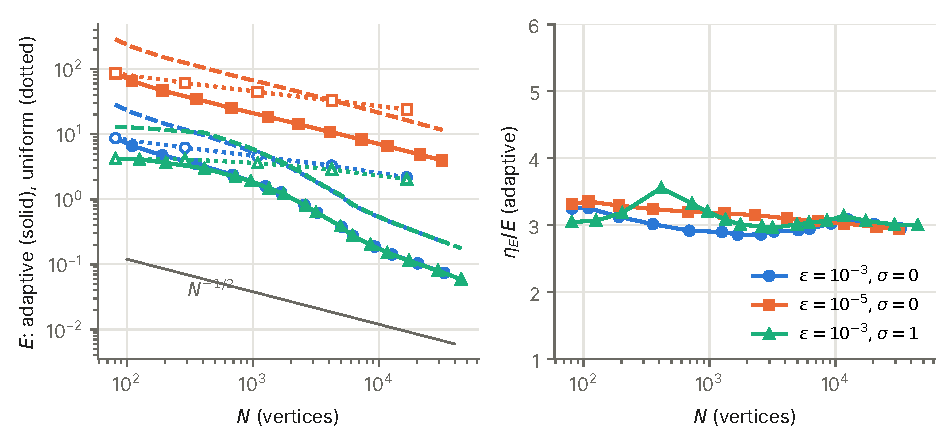
\includegraphics[width=\textwidth]{figures/sv_adapt.pdf}
\caption{Adaptive refinement, layers problem, BJK. Left: $E$ for adaptive (solid) and uniform (dotted, open
markers) refinement, and $\eta_E$ for the adaptive runs (dashed). Right: $I_E$ along the adaptive runs.}
\label{fig:adapt}
\end{figure}

\begin{figure}[!htbp]
\centering
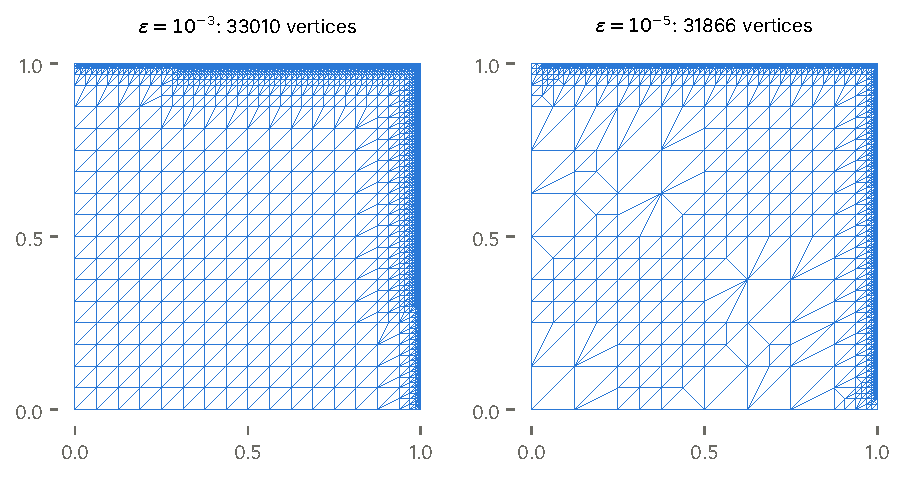
\includegraphics[width=\textwidth]{figures/sv_adapt_mesh.pdf}
\caption{Final adaptive meshes, layers problem, $\sigma=0$.}
\label{fig:adaptmesh}
\end{figure}

\subsection{\adapt{Uniform versus adaptive refinement}}\label{sec:num-unad}
{\color{magenta}

We repeat the uniform-mesh studies of Tables~\ref{tab:conv} and~\ref{tab:sweep} with adaptive refinement:
the same problems, the same marking as in Section~\ref{sec:num-adapt}, from the $8\times8$ mesh up to
$N\approx2\cdot10^4$ (Table~\ref{tab:conv}) and $N\approx10^4$ (Table~\ref{tab:sweep}). For the robustness
sweep we compare at equal cost: the adaptive loop whose $N$ is closest to $N=1089$, the size of the $32\times32$
mesh of Table~\ref{tab:sweep}.

\paragraph{Refinement studies (Figure~\ref{fig:aconv}).}
\begin{itemize}
  \item \textbf{Effectivity.} Along the adaptive runs $I_E$ lies in $2.83$--$4.18$ and tends to the same values
  as on uniform meshes, about $3.0$--$3.2$. The bound held in every loop.
  \item \textbf{Accuracy.} For the smooth solution, adaptive refinement gains nothing: at $N=16\,641$ the two
  errors agree to within $1\,\%$, and $E$ converges at the rate $1$ in both cases. For the layers problem the
  uniform error is $5.4$ ($\eps=10^{-2}$) and $5.9$ ($\eps=10^{-4}$) times the adaptive one at the same $N$.
  For $\eps=10^{-4}$, $E$ converges at the rate $0.47$ under uniform refinement and at $1.4$--$1.9$ in the last
  adaptive loops, in which the layers become resolved.
\end{itemize}

\begin{figure}[!htbp]
\centering
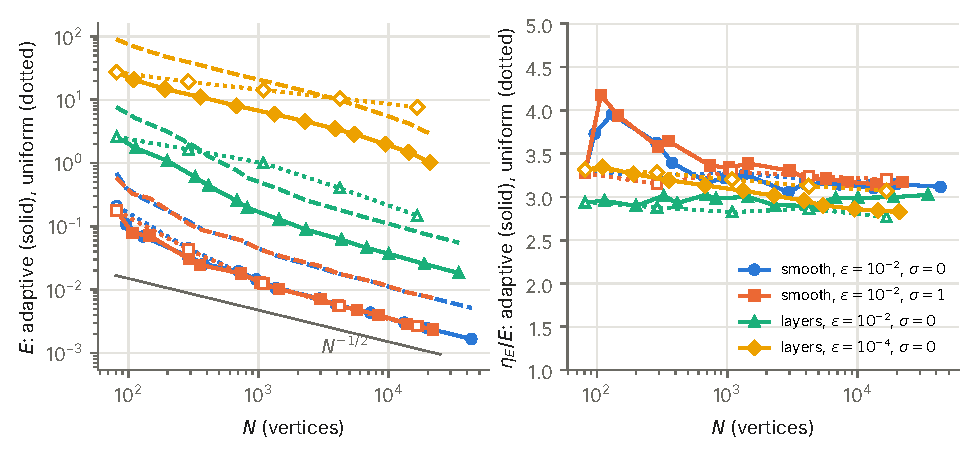
\includegraphics[width=\textwidth]{figures/sv_aconv.pdf}
\caption{\adapt{The cases of Table~\ref{tab:conv} under adaptive refinement. Left: $E$ for adaptive (solid) and uniform
(dotted, open markers) refinement, and $\eta_E$ for the adaptive runs (dashed). Right: $I_E$, adaptive (solid) and
uniform (dotted).}}
\label{fig:aconv}
\end{figure}

\paragraph{Robustness sweep (Figures~\ref{fig:abudget} and~\ref{fig:aloops}).}
\begin{itemize}
  \item \textbf{$\sigma=0$.} At equal cost, $I_E=2.89$--$3.22$ on the adaptive meshes against $2.80$--$3.23$ on the
  uniform mesh, for all $\eps$ and both stabilisations, and it stays in $2.82$--$3.35$ over all loops: the
  estimator is as robust on the meshes it generates as on the fixed mesh.
  \item \textbf{$\sigma=1$, small $\eps$.} The rise of $I_E$ to $5.4$--$5.5$ on the uniform mesh at
  $\eps\le10^{-7}$ (Section~\ref{sec:num-robust}) does not occur at equal cost on the adaptive meshes, where
  $I_E=2.75$--$3.16$. Figure~\ref{fig:aloops} shows why. The large values, up to $9.6$, appear only on the
  coarse initial mesh, and they come from the stabilisation part: $I_S=17.8$ at $N=81$ for $\eps=10^{-8}$. As the
  mesh resolves the layers, $I_S$ falls to $1.5$--$1.6$ and $I_E$ returns to about $3$. This confirms that the
  rise on the uniform mesh is a property of the under-resolved $P_2$ reference for $\|\Stil\|_*$, not of the
  estimator.
  \item \textbf{Smooth problem.} For $\eps\le10^{-3}$ the adaptive indices are higher than the uniform ones at
  equal cost: $I_E=4.0$--$5.3$ against $3.6$--$3.8$ for $\sigma=0$, and $4.5$--$6.0$ against $3.9$--$6.0$ for
  $\sigma=1$. Along the runs they reach $7.8$ after the first loop, and $10.9$ on the initial mesh. For $\sigma=1$
  and $\eps\le10^{-6}$ the fixed-point iteration reaches the iteration limit $2\cdot10^4$ on most meshes beyond
  $N\approx1100$, and the bound holds at these iterates.
  \item \textbf{Energy norm.} At $\sigma=0$ the energy-norm index still grows like $\eps^{-1}$ on the adaptive meshes,
  to $4\cdot10^5$ at $\eps=10^{-8}$ (uniform: $2.5\cdot10^6$); only the augmented measure is robust.
  \item \textbf{An open point.} For the layers problem with $\sigma=1$ and $\eps=10^{-6}$, $I_E$ rises again in the
  last loops, from $2.8$ to $4.3$, together with $I_\oplus$ (from $3.2$ to $6.6$). We have not identified the cause;
  it may be the convective part of the reference becoming resolved, and would need runs beyond $N=10^4$.
\end{itemize}

\begin{figure}[!htbp]
\centering
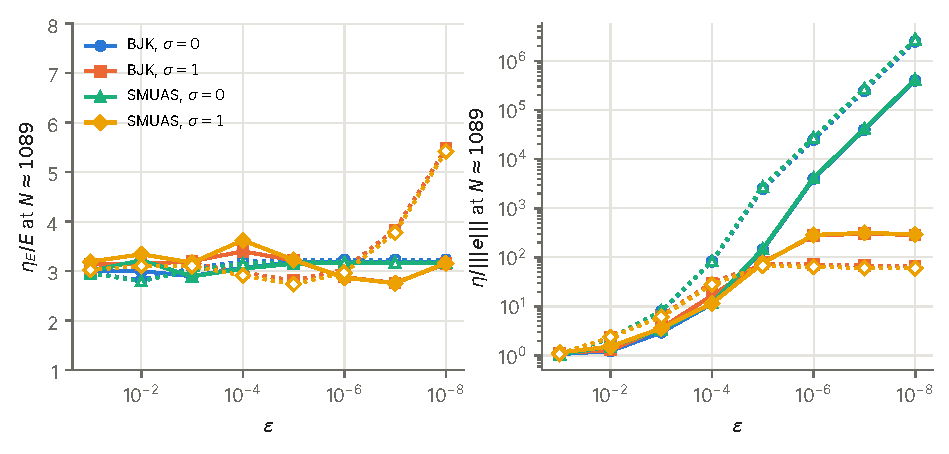
\includegraphics[width=\textwidth]{figures/sv_asweep_budget.pdf}
\caption{\adapt{The robustness sweep of Table~\ref{tab:sweep} at equal cost, layers problem: adaptive meshes with
$N\approx1089$ (solid) against the uniform $32\times32$ mesh (dotted, open markers). Left: $I_E$. Right: the
energy-norm index $\eta/\tnorm{e}$.}}
\label{fig:abudget}
\end{figure}

\begin{figure}[!htbp]
\centering
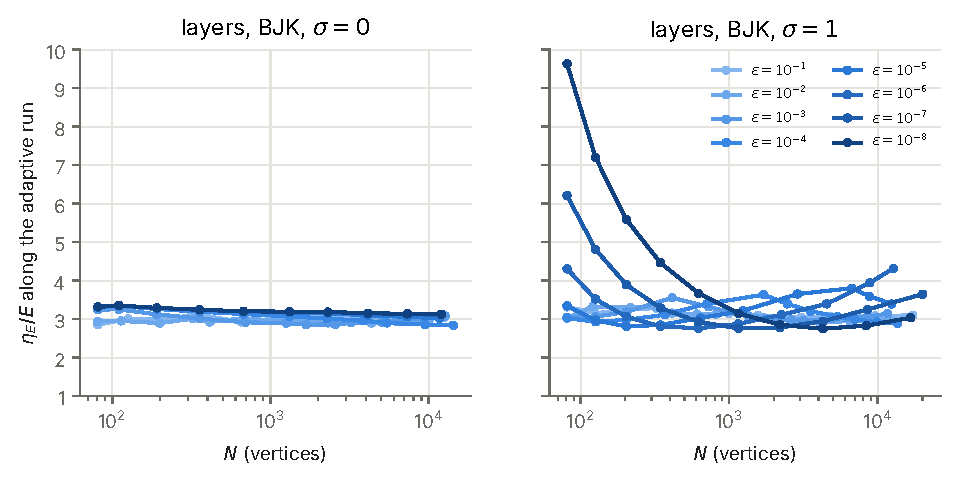
\includegraphics[width=\textwidth]{figures/sv_asweep_loops.pdf}
\caption{\adapt{$I_E$ along the adaptive runs of the robustness sweep, layers problem, BJK; one line per $\eps$, darker for
smaller $\eps$.}}
\label{fig:aloops}
\end{figure}

\paragraph{Which refinement to use.} For computing solutions, adaptive refinement is clearly preferable when the
solution has layers, by factors $4$--$18$ in $E$ at equal $N$, and it is what the estimator is designed for. For
testing the theory, the uniform meshes remain the primary evidence: a fixed coarse mesh keeps the layers
unresolved, which is the regime in which robustness can fail, isolates the dependence on $\eps$ and $\sigma$, and
is the only setting in which rates in $h$ are meaningful. The adaptive runs confirm that the effectivity stays at
about $3$ on the meshes the estimator generates itself.
}% end of the magenta block

\subsection{Inexact iterates and adaptive stopping}\label{sec:num-stop}

\paragraph{Iterates.} Table~\ref{tab:iter} and Figure~\ref{fig:iter} evaluate the estimator at the
fixed-point iterates $u^i$ on the $16\times16$ mesh. The index $I_E$ stays between $2.9$ and $5.3$ at
every iterate, including the first one, where the algebraic part $\eta_{\mathrm{alg}}$ is up to $71\,\%$
of $\eta_{\mathrm{disc}}$: this is part~2 of Proposition~\ref{prop:stop}, efficiency at every iterate
without any condition on the algebraic error. The ratio $\eta_{\mathrm{alg}}/\eta_{\mathrm{disc}}$
decreases monotonically for all problems except the smooth one with $\eps=10^{-6}$ and $\sigma=0$, for
which the fixed-point iteration does not converge in $2\cdot10^4$ iterations; there the ratio stalls
between $10^{-3}$ and $4\cdot10^{-3}$. In that case the error is smallest at $i\approx10$, $E(u^{10})=4.8$, and grows to
$8.4$ at $i=2\cdot10^4$: further iterations make the iterate worse in $E$, and the estimator, which is
efficient at every iterate, reflects this.

% generated by examples/convection_diffusion/sv_numerics/make_figures.py; do not edit
\begin{table}[!htbp]
\centering
\small
\setlength{\tabcolsep}{4pt}
\caption{Fixed-point iterates $u^i$, $i\in\{1,2,5,\dots,1000\}$ below the converged count, and the converged solution; BJK, $n=16$. The split is $\eta_{\mathrm{disc}}=\eta_E-\eta_{\mathrm{alg}}$.}\label{tab:iter}
\begin{tabular}{lrrrlrrl}
\toprule
problem & $\eps$ & $\sigma$ & it.\ to tol. & $\eta_E/E$ over $i$ & $\max_i\eta_{\mathrm{alg}}/\eta_{\mathrm{disc}}$ & $E(u^1)/E(u^{\mathrm{last}})$ & $E\le\eta_E$\\
\midrule
smooth & $10^{-2}$ & 0 & 39 & 3.24--3.63 & 0.71 & 1.81 & yes\\
smooth & $10^{-2}$ & 1 & 37 & 3.15--3.45 & 0.51 & 1.58 & yes\\
smooth & $10^{-6}$ & 0 & 20000 & 3.76--4.61 & 0.58 & 1.06 & yes\\
smooth & $10^{-6}$ & 1 & 664 & 4.42--5.28 & 0.19 & 1.20 & yes\\
layers & $10^{-2}$ & 0 & 47 & 2.88--2.97 & 0.02 & 1.01 & yes\\
layers & $10^{-2}$ & 1 & 45 & 3.32--3.33 & 0.01 & 1.01 & yes\\
layers & $10^{-6}$ & 0 & 635 & 3.29--3.47 & 0.04 & 1.01 & yes\\
layers & $10^{-6}$ & 1 & 502 & 3.51--3.56 & 0.02 & 1.03 & yes\\
\bottomrule
\end{tabular}
\end{table}


\begin{figure}[!htbp]
\centering
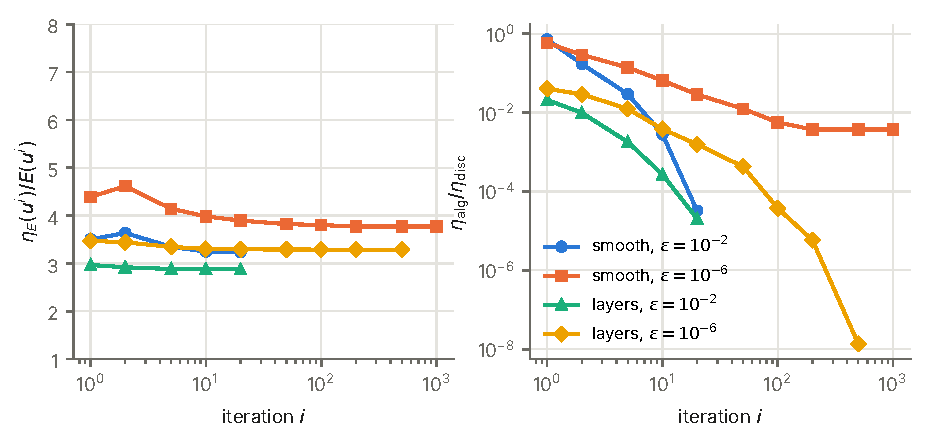
\includegraphics[width=\textwidth]{figures/sv_iter.pdf}
\caption{Fixed-point iterates, BJK, $\sigma=0$, $n=16$. Left: $I_E$ at the iterate $u^i$. Right: the
ratio $\eta_{\mathrm{alg}}/\eta_{\mathrm{disc}}$ (points with a ratio below $10^{-8}$ are omitted).}
\label{fig:iter}
\end{figure}

\paragraph{Adaptive stopping.} Table~\ref{tab:stop} runs five adaptive loops \refe{as in} Section~\ref{sec:num-adapt}
in which the fixed-point iteration is stopped either at the fixed tolerance $\|r\|\le10^{-10}\sqrt N$ or by
the criterion \eqref{eq:stop}, $\eta_{\mathrm{alg}}\le\gamma\eta_{\mathrm{disc}}$, with
$\eta_{\mathrm{disc}}=\eta_E-\eta_{\mathrm{alg}}$; each loop starts from the zero initial guess.
\begin{itemize}
  \item \textbf{Savings.} With $\gamma=0.1$, the total number of iterations drops from $227$ to $25$ (smooth,
  $\eps=10^{-2}$) and from $2323$ to $25$ (layers, $\eps=10^{-4}$), by factors $9$ and $93$; with $\gamma=0.01$
  the factors are $4.5$ and $46$.
  \item \textbf{Accuracy.} The final error $E$ changes by at most $6\,\%$ ($\gamma=0.1$, layers) and by at most
  $0.3\,\%$ for $\gamma\le0.01$. The index $I_E$ stays in $3.1$--$4.8$ in all runs, and in every stopped loop
  $\eta_{\mathrm{alg}}/\eta_{\mathrm{disc}}\le\gamma$, so $E\le(1+\gamma)\eta_{\mathrm{disc}}$
  (Proposition~\ref{prop:stop}, part~3).
  \item \textbf{Non-converging iteration.} For the smooth problem with $\eps=10^{-6}$ the fixed-point
  iteration does not reach the tolerance within $10^4$ iterations on any mesh, and $50\,000$ iterations give
  $E=3.22$. The criterion with $\gamma=0.1$ stops after $5$--$15$ iterations per loop, $50$ in total, with a
  \emph{smaller} error, $E=1.98$: as in Figure~\ref{fig:iter}, the early iterates are better than the late
  ones. For $\gamma=10^{-3}$ the criterion fires in only one of the five loops, since $\eta_{\mathrm{alg}}/\eta_{\mathrm{disc}}$ stalls
  at about $3\cdot10^{-3}$; this is a property of the iteration, not of the estimator.
\end{itemize}

% generated by examples/convection_diffusion/sv_numerics/make_figures.py; do not edit
\begin{table}[!htbp]
\centering
\footnotesize
\setlength{\tabcolsep}{4pt}
\caption{Adaptive stopping in five adaptive loops (dual marking by the SV indicators, red--green refinement), BJK, $\sigma=0$. ``tol.'' is the fixed tolerance $\|r\|\le10^{-10}\sqrt N$; otherwise the iteration stops at $\eta_{\mathrm{alg}}\le\gamma\eta_{\mathrm{disc}}$ (at most $10^4$ iterations). The last column says whether every loop stopped before the iteration limit.}\label{tab:stop}
\begin{tabular}{lrrrrlllr}
\toprule
problem & $\eps$ & $\gamma$ & it./loop & total & $E$ (last) & $\eta_E/E$ & $\max\eta_{\mathrm{alg}}/\eta_{\mathrm{disc}}$ & stopped\\
\midrule
smooth & $10^{-2}$ & tol. & 30--59 & 227 & $2.550\cdot10^{-2}$ & 3.29--3.95 & $5.78\cdot10^{-8}$ & yes\\
smooth & $10^{-2}$ & 0.1 & 5 & 25 & $2.554\cdot10^{-2}$ & 3.41--3.97 & $5.07\cdot10^{-2}$ & yes\\
smooth & $10^{-2}$ & 0.01 & 10 & 50 & $2.551\cdot10^{-2}$ & 3.33--3.98 & $7.27\cdot10^{-3}$ & yes\\
smooth & $10^{-2}$ & 0.001 & 10--20 & 80 & $2.551\cdot10^{-2}$ & 3.29--3.96 & $9.89\cdot10^{-4}$ & yes\\
smooth & $10^{-6}$ & tol. & 10000 & 50000 & $3.218$ & 3.77--4.58 & $3.03\cdot10^{-3}$ & no\\
smooth & $10^{-6}$ & 0.1 & 5--15 & 50 & $1.984$ & 4.04--4.79 & $9.83\cdot10^{-2}$ & yes\\
smooth & $10^{-6}$ & 0.01 & 120--760 & 2190 & $2.749$ & 3.80--4.45 & $9.10\cdot10^{-3}$ & yes\\
smooth & $10^{-6}$ & 0.001 & 7320--10000 & 47320 & $3.218$ & 3.77--4.58 & $3.03\cdot10^{-3}$ & no\\
layers & $10^{-4}$ & tol. & 385--628 & 2323 & $8.044$ & 3.13--3.34 & $3.57\cdot10^{-9}$ & yes\\
layers & $10^{-4}$ & 0.1 & 5 & 25 & $8.524$ & 3.20--3.42 & $2.49\cdot10^{-2}$ & yes\\
layers & $10^{-4}$ & 0.01 & 10 & 50 & $8.023$ & 3.15--3.38 & $8.43\cdot10^{-3}$ & yes\\
layers & $10^{-4}$ & 0.001 & 25--50 & 175 & $8.04$ & 3.14--3.35 & $9.29\cdot10^{-4}$ & yes\\
\bottomrule
\end{tabular}
\end{table}


\subsection{Variable diffusion}\label{sec:num-vareps}

Table~\ref{tab:vareps} reports the variable-diffusion problems on the meshes $n=8,16,32$. All bounds are
guaranteed. For the smooth coefficient, the oscillation $\eta_\eps$ converges at the rate $2.09$--$2.13$
in $h$, in accordance with Lemma~\ref{lem:V}(iii), and is at most $12\,\%$ of $\eta$ (at contrast $10^4$ on
the coarsest mesh). For the jump aligned with the mesh, $\Pi_1\eps=\eps$ and $\eta_\eps=0$. The
effectivity $I_E$ lies in $2.6$--$4.5$ for contrasts up to $10^4$, for $\eps=10^{-2}$ and $10^{-6}$ alike. For
the jump it does not grow with the contrast; for the smooth coefficient it grows mildly, from
$3.1$ at contrast $1$ to at most $4.3$ at contrast $10^4$ (on the coarsest mesh). This is the quasi-monotone case; the constants of
Theorem~\ref{thm:vareps} depend on the patch contrast, but for an aligned jump that contrast does not
show up in the indices. Checkerboard (non-quasi-monotone) coefficients are not tested; for them no
local estimator can be robust \cite{Li26}.

% generated by examples/convection_diffusion/sv_numerics/make_figures.py; do not edit
\begin{table}[!htbp]
\centering
\footnotesize
\setlength{\tabcolsep}{4pt}
\caption{Variable diffusion, BJK, $\sigma=0$, $n\in\{8,16,32\}$: ranges over the three meshes. The rate is that of $\eta_\eps$ with respect to $N^{-1/2}$ between $n=16$ and $n=32$ (expected: $2$).}\label{tab:vareps}
\begin{tabular}{lrrllllrl}
\toprule
$\eps(x)$ & $\eps$ & contrast & $I$ & $I_\oplus$ & $I_E$ & $\max\eta_\eps/\eta$ & rate & $E\le\eta_E$\\
\midrule
smooth & $10^{-2}$ & 1 & 1.23--4.58 & 3.30--4.06 & 3.07--3.13 & 0.000 & --- & yes\\
smooth & $10^{-2}$ & 100 & 1.07--1.24 & 3.16--3.39 & 3.15--3.26 & 0.035 & 2.09 & yes\\
smooth & $10^{-2}$ & 10000 & 1.10--1.44 & 3.30--4.28 & 3.29--4.27 & 0.117 & 2.09 & yes\\
smooth & $10^{-6}$ & 1 & 7959--36796 & 3.72--5.01 & 3.50--3.70 & 0.000 & --- & yes\\
smooth & $10^{-6}$ & 100 & 818--3354 & 3.73--5.44 & 3.54--4.03 & 0.000 & 2.13 & yes\\
smooth & $10^{-6}$ & 10000 & 64.07--336 & 4.31--5.49 & 3.94--4.46 & 0.001 & 2.10 & yes\\
jump & $10^{-2}$ & 100 & 2.56--7.63 & 3.43--4.18 & 2.61--2.99 & 0.000 & --- & yes\\
jump & $10^{-2}$ & 10000 & 2.61--8.12 & 3.43--4.22 & 2.60--3.01 & 0.000 & --- & yes\\
jump & $10^{-6}$ & 100 & 9025--28125 & 4.75--5.12 & 3.44--3.54 & 0.000 & --- & yes\\
jump & $10^{-6}$ & 10000 & 2156--4989 & 4.78--5.08 & 3.41--3.52 & 0.000 & --- & yes\\
\bottomrule
\end{tabular}
\end{table}


\subsection{Three dimensions}\label{sec:num-3d}

Table~\ref{tab:d3} repeats the uniform-refinement study on the unit cube ($n=4,8,16$, up to $N=4913$
vertices and $24\,576$ tetrahedra).
\begin{itemize}
  \item \textbf{Layers.} $I_E=2.94$--$3.55$ for $\eps=10^{-2}$ and $10^{-6}$, as in two dimensions; $I_\oplus\le4.9$
  and $I_S=1.21$--$1.26$.
  \item \textbf{Smooth solution.} $I_E$ is higher than in two dimensions, $5.1$--$6.4$, but decreases under
  refinement for both values of $\eps$ ($5.97\to5.40$ and $6.39\to5.09$). These meshes are coarse: $E$ still
  converges at the pre-asymptotic rates $2.1$--$2.7$ in $h$, dominated by the stabilisation part
  $\|\Stil\|_*$, which is estimated sharply ($I_S=1.28$--$1.31$); the larger index comes from the convective
  dual norm on coarse tetrahedral meshes. For $\eps=10^{-6}$ on the finest mesh the fixed-point iteration does
  not converge within $2\cdot10^4$ iterations, and the bound still holds at the last iterate.
  \item \textbf{Energy norm.} As in two dimensions, $I$ is useless for $\sigma=0$ and small $\eps$
  ($1.0\cdot10^4$--$1.4\cdot10^5$ at $\eps=10^{-6}$, against $2.6$--$9.3$ at $\eps=10^{-2}$), while $I_E$ is not
  affected.
  \item \textbf{Cost.} The estimator takes about $8$\,s at $N=729$ and $220$--$240$\,s at $N=4913$ in our
  Python implementation; the cost is dominated by the vertex-patch problems in $\RTN$, whose size grows
  quickly with the number of tetrahedra per patch in three dimensions. The patch problems are independent and
  can be solved in parallel; the global $\RT_0$ defect problem takes a small fraction of the time.
\end{itemize}

% generated by examples/convection_diffusion/sv_numerics/make_figures.py; do not edit
\begin{table}[!htbp]
\centering
\small
\setlength{\tabcolsep}{4pt}
\caption{Three dimensions, uniform refinement of the unit cube, BJK, $\sigma=0$. Rates with respect to $N^{-1/3}\sim h$; the last column is the time of the estimator in seconds.}\label{tab:d3}
\begin{tabular}{lrrlrrrrr}
\toprule
problem & $\eps$ & $N$ & $E$ & rate & $I$ & $I_\oplus$ & $I_E$ & time\\
\midrule
smooth & $10^{-2}$ & 125 & $0.7$ &  & 9.27 & 7.82 & 5.97 & 0.7\\
smooth & $10^{-2}$ & 729 & $0.144$ & 2.69 & 4.83 & 6.98 & 5.71 & 9.0\\
smooth & $10^{-2}$ & 4913 & $3.55\cdot10^{-2}$ & 2.20 & 2.64 & 5.84 & 5.40 & 226.6\\
smooth & $10^{-6}$ & 125 & $6.72\cdot10^{1}$ &  & $7.4\cdot10^{4}$ & 9.26 & 6.39 & 0.6\\
smooth & $10^{-6}$ & 729 & $2.00\cdot10^{1}$ & 2.06 & $2.8\cdot10^{4}$ & 6.93 & 5.31 & 8.4\\
smooth & $10^{-6}$ & 4913 & $4.06$ & 2.51 & $1.0\cdot10^{4}$ & 5.56 & 5.09 & 238.0\\
layers & $10^{-2}$ & 125 & $2.74$ &  & 6.67 & 4.01 & 3.10 & 0.6\\
layers & $10^{-2}$ & 729 & $1.82$ & 0.70 & 4.31 & 3.71 & 3.01 & 8.0\\
layers & $10^{-2}$ & 4913 & $1.14$ & 0.73 & 2.93 & 3.64 & 2.94 & 217.3\\
layers & $10^{-6}$ & 125 & $2.79\cdot10^{2}$ &  & $1.4\cdot10^{5}$ & 4.71 & 3.38 & 0.5\\
layers & $10^{-6}$ & 729 & $2.01\cdot10^{2}$ & 0.56 & $7.3\cdot10^{4}$ & 4.78 & 3.47 & 8.5\\
layers & $10^{-6}$ & 4913 & $1.35\cdot10^{2}$ & 0.63 & $3.8\cdot10^{4}$ & 4.93 & 3.55 & 236.1\\
\bottomrule
\end{tabular}
\end{table}


\subsection{Summary}

The experiments answer the questions (Q1)--(Q7) as follows.
\begin{enumerate}[label=(Q\arabic*)]
  \item The bound $E\le\eta_E$ held in every run: two and three dimensions, both stabilisations,
  $\eps=10^{-1},\dots,10^{-8}$, $\sigma\in\{0,1\}$, variable reaction and diffusion, adaptive meshes and inexact
  iterates\refe{, and so did $I\ge1$, $I_\oplus\ge1$ and $I_S\ge1$. Since the references are lower bounds of the dual
  norms, this is a consistency check rather than a proof}.
  \item For constant coefficients, $I_E$ lies in $2.6$--$5.3$ in two dimensions, inexact iterates included,
  independently of $\eps$, $\sigma$, the stabilisation and the mesh; the only exception is a rise to $6.0$
  ($n=32$) and $7.1$ ($n=16$) at $\sigma=1$, $\eps\le10^{-7}$, \adapt{which the adaptive runs identify as an
  under-resolved reference for $\|\Stil\|_*$ (Section~\ref{sec:num-unad})}\asref{, as the asymptotically exact
  reference \eqref{eq:Sasym} confirms ($I_S=1.6$--$2.2$ and $\eta_E/E=8.3$--$10.2$ for $\theta$ down to $10^{-5}$)}; in three dimensions it is $2.9$--$6.4$ and
  decreases under refinement. The energy-norm index $I$, and the guaranteed bound of \cite{ABR17}, are not
  robust.
  \item The effectivity grows with $c_b$, at most linearly for $\eta_{E,c}$ and well below $c_b^2$ for $\eta_E$:
  a variable reaction with a small lower bound is the one case in which robustness is lost, as the theory
  predicts.
  \item The local ratio $\max_K\eta_K^2/E_{\mathrm{loc}}(\tilde\omega_K)^2$ is at most $0.51$.
  \item Adaptive refinement driven by $\eta_K$ resolves the layers and reduces $E$ by factors $4$--$18$
  against uniform refinement at equal $N$, with $I_E=2.9$--$3.6$ throughout. \adapt{Repeating the refinement and
  robustness studies adaptively gives the same effectivity, about $3$, as on uniform meshes.}
  \item The estimator is efficient at every iterate, and the stopping criterion saves up to $99\,\%$ of the
  iterations at a change of the error of at most $6\,\%$ ($\gamma=0.1$) or $0.3\,\%$ ($\gamma\le0.01$).
  \item For variable diffusion, $\eta_\eps$ converges at rate $2$ and $I_E$ stays in $2.6$--$4.5$ up to contrast
  $10^4$.
\end{enumerate}

\paragraph{Reproducibility.} All results are produced by the scripts \texttt{run\_numerics.py} and
\texttt{make\_figures.py} in the directory
\path{examples/convection_diffusion/sv_numerics} of \texttt{galerkit}. The first runs the experiments (about
$35$ minutes on four cores, the three-dimensional runs sequentially because of their memory use); the
second writes the tables, the figures and, for every stored solution, a VTK file
(\texttt{.vtu}) with $u_h$, $u$, $u-u_h$, $\eps$, $\eta_K$, $\tnorm{e}_K$ and the local effectivity
$\eta_K/\tnorm{e}_K$. \adapt{The figures of Section~\ref{sec:num-unad} are produced by
\texttt{make\_adaptive\_figures.py} in the same directory.}

).
% Data: examples/convection_diffusion/sv_numerics/run_numerics.py (output/*.json);
% tables and figures: make_figures.py -> tables/*.tex, figures/sv_*.{pdf,png}.
% All numbers quoted in the text below are read off those tables.

% ===========================================================================
\section{Numerical experiments}\label{sec:num}
% ===========================================================================

We test the estimator against the exact error. The questions are the ones raised by the theory:
\begin{enumerate}[label=(Q\arabic*)]
  \item Is the bound guaranteed, $E\le\eta_E$, in every run (Theorem~\ref{thm:rel})?
  \item Are the effectivity indices bounded independently of $\eps$, $\sigma$ and the stabilisation
  (Theorem~\ref{thm:eff}, Corollary~\ref{cor:two}), and do they stay bounded under refinement?
  \item Does the dependence on $c_b$ follow Corollaries~\ref{cor:two} and~\ref{cor:twoc}?
  \item Is the estimator locally efficient in the localisable measure (Theorem~\ref{thm:loc})?
  \item Do the indicators drive adaptive refinement to the optimal rate?
  \item Are the bounds valid at inexact iterates, and does the stopping criterion of
  Proposition~\ref{prop:stop} save iterations without spoiling the error?
  \item Does the variable-diffusion version keep its effectivity, with $\eta_\eps=O(h^2)$
  (Theorem~\ref{thm:vareps})?
\end{enumerate}

\subsection{Setup}

\paragraph{Discretisation.} Conforming $P_1$ elements on uniform meshes of the unit square
($n\times n$ squares, each cut into two triangles; $N=(n+1)^2$ vertices) or the unit cube ($n^3$
cubes, each cut into six tetrahedra), and on red--green refined meshes in the adaptive runs. The
stabilisations are the AFC scheme with the limiter of \cite{BJK17} (BJK), and the symmetrised
monotone upwind-type algebraic stabilisation of \cite{Kn23} (SMUAS). The nonlinear problem is solved
by the damped fixed-point iteration of \cite{AJ27} up to $\|r\|\le10^{-10}\sqrt N$, with at most
$2\cdot10^4$ iterations, unless stated otherwise.

\paragraph{Test problems} (all with $b$ constant, so $\sigma=c$, $c_b=1$ and $\kappa=3$, except in
Section~\ref{sec:num-cb}).
\begin{itemize}
  \item \emph{smooth}: $u=\prod_i\sin(\pi x_i)+x_1^2\prod_{i>1}x_i$, $b=(1,\tfrac12)$ or
  $(1,\tfrac12,\tfrac14)$, Dirichlet data on $\partial\Omega$; $f$ is computed from $u$. The solution
  has no layers, so its error is not dominated by layers, but for small $\eps$ the scheme is
  convection-dominated on every mesh used.
  \item \emph{layers}: $u=\prod_iw(x_i)$ with
  $w(s)=s-\bigl(e^{(s-1)/\eps}-e^{-1/\eps}\bigr)/\bigl(1-e^{-1/\eps}\bigr)$, $b=(1,\dots,1)$, homogeneous
  Dirichlet data; $u$ has exponential layers of width $\eps$ at the outflow boundary $x_i=1$.
  \item \emph{variable diffusion}: $u=\phi(x_1)\prod_{i>1}4x_i(1-x_i)$, either with
  $\eps(x)=\eps\,k^{x_1}$, $\phi(s)=4s(1-s)$ (\emph{smooth}), or with $\eps$ jumping from $\eps$ to $k\eps$
  at $x_1=\frac12$ and $\phi$ chosen such that the flux $\eps\phi'$ is continuous (\emph{jump}); $k$ is
  the contrast.
\end{itemize}

\paragraph{Error measures.} $\tnorm{e}$ is computed with a quadrature of degree~8. The dual norms
$\|B_A'(e,\cdot)\|_*$ and $\|\Stil\|_*$, and the local dual norms of $E_{\mathrm{loc}}$, are computed
from their Riesz representatives in the $P_2$ space on the same mesh (on each vertex patch for
$E_{\mathrm{loc}}$). These are \emph{lower} bounds of the true dual norms, so the reported effectivity
indices are slight overestimates; they become crude when the dual norm concentrates in layers that
the mesh does not resolve (see Section~\ref{sec:num-robust}). We report the effectivity indices
\[
  I=\frac{\eta}{\tnorm{e}},\qquad I_\oplus=\frac{\kappa\eta}{\tnorm{e}_\oplus},\qquad
  I_S=\frac{\eta_S}{\|\Stil\|_*},\qquad I_E=\frac{\eta_E}{E},
\]
of which $I_E$ is the one covered by Corollary~\ref{cor:two}; $I_\oplus\ge1$ and $I\ge1$ are guaranteed
too, but only $I_\oplus$ is expected to be robust.

\subsection{Solutions and indicators}

Figure~\ref{fig:snap} shows the discrete solution of the layers problem for $\eps=10^{-3}$ on the
$32\times32$ mesh, the cell indicators $\eta_K=\eta_{A,K}+\eta_{S,K}$, and the local energy errors
$\tnorm{e}_K$. The mesh does not resolve the layers ($h\approx4.4\cdot10^{-2}\gg\eps$); the AFC
solution is free of oscillations, and both the indicators and the error concentrate in the cells at
the outflow boundary, with a decay of several orders of magnitude into the interior. The indicator
is larger than $\tnorm{e}_K$ in the layer cells: it measures the residual in the dual norm, which
contains the convective part $\|B_A'(e,\cdot)\|_*$ of the error.

\begin{figure}[!htbp]
\centering
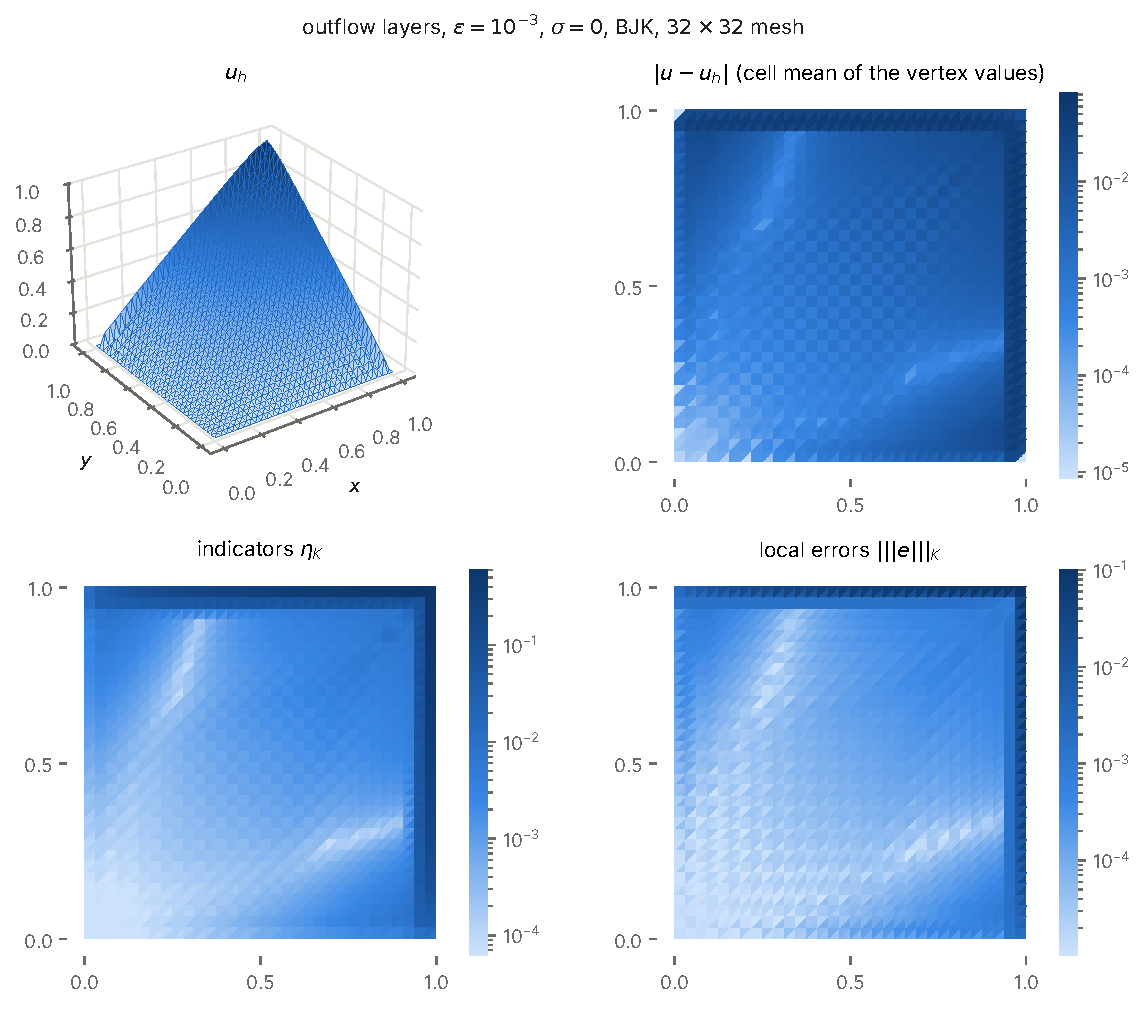
\includegraphics[width=\textwidth]{figures/sv_snap.pdf}
\caption{Layers problem, $\eps=10^{-3}$, $\sigma=0$, BJK, $n=32$: discrete solution $u_h$, indicators
$\eta_K$ and local errors $\tnorm{e}_K$ (logarithmic colour scale, common to both).}
\label{fig:snap}
\end{figure}

\subsection{Uniform refinement}\label{sec:num-conv}

Table~\ref{tab:conv} and Figure~\ref{fig:conv} report uniform refinement from $n=8$ to $n=128$.
\begin{itemize}
  \item \textbf{Smooth solution, $\eps=10^{-2}$.} $E$ and $\eta_E$ converge at the optimal rate $1$ in
  $h$ once the mesh resolves the solution; on the coarse meshes both decrease faster, because the
  stabilisation term $\|\Stil\|_*$ dominates $E$ there and decreases at a higher rate. The effectivity
  $I_E$ lies between $3.15$ and $3.29$ for $\sigma=0$ and $\sigma=1$ alike. The energy-norm index $I$
  tends to $1.1$: in the diffusion-dominated regime the energy norm and the dual norm of the
  residual coincide asymptotically.
  \item \textbf{Layers, $\eps=10^{-2}$.} The layers are resolved only from $n=64$ on, and the
  convergence of $E$ accelerates accordingly; $I_E$ stays between $2.77$ and $2.94$.
  \item \textbf{Layers, $\eps=10^{-4}$.} The meshes never resolve the layers. The energy error
  $\tnorm{e}$ \emph{increases} under refinement, because the error, concentrated in the outflow
  cells, sees an increasing part of the layer, while $E$ is dominated by the convective dual norm and
  decreases at the rate $0.45$--$0.53$; $\eta_E$ follows it with the rate $0.49$--$0.55$. The index $I_E$
  is $3.07$--$3.31$ on every mesh, whereas the energy-norm index $I$ falls from $833$ to $18.7$: the
  energy-norm bound is guaranteed but useless in this regime, which is why the error is measured in
  $E$.
\end{itemize}

% generated by examples/convection_diffusion/sv_numerics/make_figures.py; do not edit
\begin{table}[!htbp]
\centering
\small
\setlength{\tabcolsep}{4pt}
\caption{Uniform refinement in 2D, BJK. Rates with respect to $N^{-1/2}\sim h$; the expected rate is $1$ once the mesh resolves the solution. Effectivity indices $I=\eta/\tnorm{e}$, $I_\oplus=\kappa\eta/\tnorm{e}_\oplus$, $I_E=\eta_E/E$; the last column is the number of fixed-point iterations.}\label{tab:conv}
\begin{tabular}{rlllrlrrrr}
\toprule
$N$ & $\tnorm{e}$ & $E$ & rate & $\eta_E$ & rate & $I$ & $I_\oplus$ & $I_E$ & it.\\
\midrule
\multicolumn{10}{l}{\emph{smooth, $\eps=10^{-2}$, $\sigma=0$}}\\
81 & $4.88\cdot10^{-2}$ & $0.209$ &  & $0.687$ &  & 4.12 & 4.22 & 3.29 & 59\\
289 & $2.15\cdot10^{-2}$ & $4.48\cdot10^{-2}$ & 2.42 & $0.145$ & 2.45 & 2.05 & 3.86 & 3.24 & 39\\
1089 & $1.04\cdot10^{-2}$ & $1.26\cdot10^{-2}$ & 1.91 & $4.15\cdot10^{-2}$ & 1.89 & 1.31 & 3.46 & 3.28 & 18\\
4225 & $5.16\cdot10^{-3}$ & $5.51\cdot10^{-3}$ & 1.23 & $1.76\cdot10^{-2}$ & 1.26 & 1.14 & 3.24 & 3.20 & 9\\
16641 & $2.58\cdot10^{-3}$ & $2.65\cdot10^{-3}$ & 1.07 & $8.40\cdot10^{-3}$ & 1.08 & 1.09 & 3.18 & 3.17 & 6\\
\multicolumn{10}{l}{\emph{smooth, $\eps=10^{-2}$, $\sigma=1$}}\\
81 & $5.01\cdot10^{-2}$ & $0.178$ &  & $0.582$ &  & 3.34 & 4.04 & 3.27 & 56\\
289 & $2.16\cdot10^{-2}$ & $4.31\cdot10^{-2}$ & 2.23 & $0.136$ & 2.29 & 1.89 & 3.69 & 3.15 & 37\\
1089 & $1.04\cdot10^{-2}$ & $1.25\cdot10^{-2}$ & 1.87 & $4.12\cdot10^{-2}$ & 1.80 & 1.29 & 3.46 & 3.29 & 18\\
4225 & $5.16\cdot10^{-3}$ & $5.47\cdot10^{-3}$ & 1.22 & $1.77\cdot10^{-2}$ & 1.24 & 1.15 & 3.29 & 3.24 & 9\\
16641 & $2.58\cdot10^{-3}$ & $2.64\cdot10^{-3}$ & 1.06 & $8.45\cdot10^{-3}$ & 1.08 & 1.10 & 3.22 & 3.20 & 6\\
\multicolumn{10}{l}{\emph{layers, $\eps=10^{-2}$, $\sigma=0$}}\\
81 & $0.522$ & $2.6$ &  & $7.62$ &  & 4.19 & 3.78 & 2.94 & 67\\
289 & $0.471$ & $1.64$ & 0.72 & $4.72$ & 0.75 & 2.88 & 3.64 & 2.88 & 47\\
1089 & $0.366$ & $1$ & 0.74 & $2.83$ & 0.77 & 2.21 & 3.56 & 2.82 & 63\\
4225 & $0.231$ & $0.401$ & 1.35 & $1.15$ & 1.33 & 1.52 & 3.26 & 2.86 & 28\\
16641 & $0.127$ & $0.148$ & 1.46 & $0.409$ & 1.51 & 1.07 & 2.77 & 2.77 & 9\\
\multicolumn{10}{l}{\emph{layers, $\eps=10^{-4}$, $\sigma=0$}}\\
81 & $3.07\cdot10^{-2}$ & $2.72\cdot10^{1}$ &  & $9.02\cdot10^{1}$ &  & 833.01 & 4.76 & 3.31 & 405\\
289 & $6.15\cdot10^{-2}$ & $1.94\cdot10^{1}$ & 0.53 & $6.37\cdot10^{1}$ & 0.55 & 290.45 & 4.81 & 3.28 & 709\\
1089 & $0.154$ & $1.42\cdot10^{1}$ & 0.47 & $4.56\cdot10^{1}$ & 0.51 & 82.17 & 4.75 & 3.20 & 700\\
4225 & $0.242$ & $1.05\cdot10^{1}$ & 0.45 & $3.27\cdot10^{1}$ & 0.49 & 37.26 & 4.65 & 3.12 & 626\\
16641 & $0.342$ & $7.6$ & 0.47 & $2.33\cdot10^{1}$ & 0.49 & 18.72 & 4.54 & 3.07 & 566\\
\bottomrule
\end{tabular}
\end{table}


\begin{figure}[!htbp]
\centering
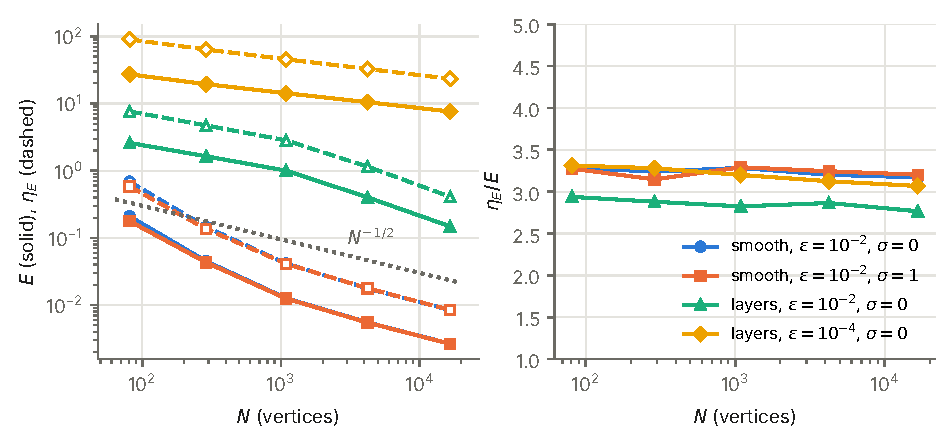
\includegraphics[width=\textwidth]{figures/sv_conv.pdf}
\caption{Uniform refinement in 2D, BJK. Left: $E$ (solid) and $\eta_E$ (dashed, open markers).
Right: effectivity index $I_E=\eta_E/E$.}
\label{fig:conv}
\end{figure}

\subsection{Robustness in \texorpdfstring{$\eps$}{eps}, \texorpdfstring{$\sigma$}{sigma} and the stabilisation}\label{sec:num-robust}

Table~\ref{tab:sweep} and Figure~\ref{fig:sweep} sweep $\eps$ from $10^{-1}$ to $10^{-8}$ on the fixed
mesh $n=32$, for $\sigma\in\{0,1\}$, both stabilisations and both problems.
\begin{itemize}
  \item \textbf{$\sigma=0$.} $I_E$ lies in $2.80$--$3.23$ for the layers problem and in $3.15$--$3.78$
  for the smooth problem, and becomes constant for $\eps\le10^{-5}$. $I_\oplus$ stays below $4.9$,
  and the stabilisation part is estimated sharply, $I_S=1.21$--$1.34$. BJK and SMUAS give the
  same indices $I_E$ and $I_\oplus$ to within $3\,\%$, as Remark~\ref{rem:robust} predicts: the limiter enters only
  through the functional, not the constants.
  \item \textbf{Energy norm.} The energy-norm index $I$ grows like $\eps^{-1}$ for $\sigma=0$, up to
  $2.5\cdot10^6$ at $\eps=10^{-8}$; the guaranteed energy-norm bound of \cite{ABR17} behaves in the
  same way. For $\sigma=1$, $I$ saturates at about $60$--$90$, the reaction giving $L^2$ control, while
  the ABR17 bound keeps growing ($1.3\cdot10^4$ at $\eps=10^{-8}$), because its reaction cut-off is not
  robust.
  \item \textbf{$\sigma=1$, small $\eps$.} Down to $\eps=10^{-6}$, $I_E$ stays in $2.7$--$3.2$ for the
  layers problem and in $3.2$--$4.9$ for the smooth one. For $\eps<10^{-6}$ it rises, to $5.5$ (layers)
  and $6.0$ (smooth) at $\eps=10^{-8}$. This increase comes from $I_S$ ($7.8$ and $10.4$ at
  $\eps=10^{-8}$), while $I_\oplus$ \emph{decreases}. This is consistent with a
  reference effect rather than with a loss of robustness: for $\sigma>0$, the Riesz representative of
  $\Stil$ has layers of width $(\eps/\sigma)^{1/2}=10^{-4}$, far below the mesh size $3\cdot10^{-2}$, so
  the same-mesh $P_2$ reference underestimates $\|\Stil\|_*$. Theorem~\ref{thm:eff} bounds $\eta_S$ by
  the true dual norm, independently of $\eps$. \adapt{The adaptive runs of Section~\ref{sec:num-unad} confirm this:
  once the mesh resolves the layers, $I_S$ falls to $1.5$--$1.6$ and $I_E$ to about $3$.} \asref{The
  asymptotic reference below makes this quantitative.}
\end{itemize}

% generated by examples/convection_diffusion/sv_numerics/make_figures.py; do not edit
\begin{table}[!htbp]
\centering
\footnotesize
\setlength{\tabcolsep}{4pt}
\caption{Robustness in $\eps$ and $\sigma$ on the uniform mesh with $n=32$ ($N=1089$). $I_E=\eta_E/E$, $I_\oplus=\kappa\eta/\tnorm{e}_\oplus$, $I_S=\eta_S/\|\Stil\|_*$, $I=\eta/\tnorm{e}$ and, for comparison, the effectivity $I_{\mathrm{ABR17}}$ of the guaranteed energy-norm bound of \cite{ABR17}.}\label{tab:sweep}
\begin{tabular}{llrrrrrrrr}
\toprule
case & index & $10^{-1}$ & $10^{-2}$ & $10^{-3}$ & $10^{-4}$ & $10^{-5}$ & $10^{-6}$ & $10^{-7}$ & $10^{-8}$\\
\midrule
layers, BJK, $\sigma=0$ & $I_E$ & 2.96 & 2.82 & 3.06 & 3.20 & 3.23 & 3.23 & 3.23 & 3.23\\
 & $I_\oplus$ & 2.98 & 3.56 & 4.30 & 4.75 & 4.84 & 4.84 & 4.84 & 4.84\\
 & $I_S$ & 1.26 & 1.24 & 1.24 & 1.22 & 1.22 & 1.22 & 1.22 & 1.22\\
 & $I$ & 1.06 & 2.21 & 7.95 & 82.17 & $2.5\cdot10^{3}$ & $2.5\cdot10^{4}$ & $2.5\cdot10^{5}$ & $2.5\cdot10^{6}$\\
 & $I_{\mathrm{ABR17}}$ & 1.47 & 1.93 & 6.26 & 64.53 & $1.9\cdot10^{3}$ & $1.9\cdot10^{4}$ & $1.9\cdot10^{5}$ & $1.9\cdot10^{6}$\\
\addlinespace
layers, BJK, $\sigma=1$ & $I_E$ & 3.03 & 3.13 & 3.16 & 2.97 & 2.81 & 3.04 & 3.83 & 5.47\\
 & $I_\oplus$ & 3.05 & 3.95 & 4.25 & 4.02 & 3.83 & 3.50 & 3.28 & 3.24\\
 & $I_S$ & 1.29 & 1.29 & 1.41 & 1.54 & 1.66 & 2.55 & 4.41 & 7.79\\
 & $I$ & 1.09 & 2.33 & 6.39 & 30.27 & 74.58 & 71.78 & 67.57 & 66.77\\
 & $I_{\mathrm{ABR17}}$ & 1.47 & 1.94 & 6.25 & 57.80 & 391.31 & $1.3\cdot10^{3}$ & $4.0\cdot10^{3}$ & $1.3\cdot10^{4}$\\
\addlinespace
layers, SMUAS, $\sigma=0$ & $I_E$ & 2.95 & 2.80 & 3.01 & 3.15 & 3.17 & 3.18 & 3.18 & 3.18\\
 & $I_\oplus$ & 2.97 & 3.57 & 4.29 & 4.73 & 4.82 & 4.82 & 4.82 & 4.82\\
 & $I_S$ & 1.34 & 1.24 & 1.25 & 1.23 & 1.23 & 1.23 & 1.23 & 1.23\\
 & $I$ & 1.06 & 2.26 & 8.09 & 83.92 & $2.7\cdot10^{3}$ & $2.7\cdot10^{4}$ & $2.7\cdot10^{5}$ & $2.7\cdot10^{6}$\\
 & $I_{\mathrm{ABR17}}$ & 1.47 & 1.97 & 6.38 & 65.99 & $2.2\cdot10^{3}$ & $2.2\cdot10^{4}$ & $2.2\cdot10^{5}$ & $2.2\cdot10^{6}$\\
\addlinespace
layers, SMUAS, $\sigma=1$ & $I_E$ & 3.03 & 3.10 & 3.10 & 2.91 & 2.73 & 2.97 & 3.78 & 5.42\\
 & $I_\oplus$ & 3.04 & 3.95 & 4.20 & 4.00 & 3.81 & 3.49 & 3.27 & 3.24\\
 & $I_S$ & 1.37 & 1.28 & 1.41 & 1.50 & 1.61 & 2.46 & 4.26 & 7.53\\
 & $I$ & 1.08 & 2.36 & 6.14 & 28.08 & 66.99 & 64.21 & 60.54 & 59.85\\
 & $I_{\mathrm{ABR17}}$ & 1.47 & 1.99 & 6.38 & 58.84 & 389.93 & $1.3\cdot10^{3}$ & $4.0\cdot10^{3}$ & $1.3\cdot10^{4}$\\
\addlinespace
smooth, BJK, $\sigma=0$ & $I_E$ & 3.15 & 3.28 & 3.76 & 3.78 & 3.58 & 3.58 & 3.58 & 3.58\\
 & $I_\oplus$ & 3.17 & 3.46 & 4.85 & 4.49 & 3.87 & 3.86 & 3.85 & 3.85\\
 & $I_S$ & 1.29 & 1.30 & 1.24 & 1.21 & 1.22 & 1.22 & 1.22 & 1.22\\
 & $I$ & 1.12 & 1.31 & 6.28 & 77.92 & 778.23 & $6.9\cdot10^{3}$ & $6.8\cdot10^{4}$ & $6.8\cdot10^{5}$\\
 & $I_{\mathrm{ABR17}}$ & 1.70 & 1.76 & 5.18 & 74.26 & 842.71 & $7.5\cdot10^{3}$ & $7.4\cdot10^{4}$ & $7.4\cdot10^{5}$\\
\addlinespace
smooth, BJK, $\sigma=1$ & $I_E$ & 3.22 & 3.29 & 3.86 & 4.66 & 4.93 & 4.81 & 5.04 & 6.00\\
 & $I_\oplus$ & 3.24 & 3.46 & 4.82 & 5.50 & 5.68 & 5.22 & 4.79 & 4.69\\
 & $I_S$ & 1.32 & 1.37 & 1.45 & 1.66 & 2.24 & 3.41 & 5.88 & 10.39\\
 & $I$ & 1.14 & 1.29 & 5.60 & 42.08 & 90.00 & 92.63 & 85.82 & 84.22\\
 & $I_{\mathrm{ABR17}}$ & 1.70 & 1.76 & 5.05 & 49.08 & 229.66 & 763.28 & $2.4\cdot10^{3}$ & $7.7\cdot10^{3}$\\
\bottomrule
\end{tabular}
\end{table}


{\color{teal}
\paragraph{An asymptotically exact reference for $\|\Stil\|_*$.} For $\theta\ll1$ the dual norm of the
stabilisation functional can be evaluated without resolving its Riesz representative. With
$q=A\nabla u_h$ cellwise constant, $\Stil(v)=(q,\nabla v)=-\sum_F(\jump{q\cdot n},v)_F$ for $v\in H^1_D$, since
$\dv q=0$ in each cell. Away from the vertices, the Riesz representative is a sum of one-dimensional layers
$-\eps z''+\sigma z=\jump{q\cdot n}\,\delta_F$ across the faces, each of energy
$\jump{q\cdot n}^2/(2(\eps\sigma)^{1/2})$ per unit length. Hence
\begin{equation}\label{eq:Sasym}
  \|\Stil\|_*^2=\sum_{F\text{ interior}}\frac{\|\jump{q\cdot n}\|_F^2}{2(\eps\sigma)^{1/2}}\,\bigl(1+O(\theta)\bigr),
  \qquad \theta\to0,
\end{equation}
and the same sum over the faces interior to $\tilde\omega_K$ gives $\|\Stil\|_{*,\tilde\omega_K}^2$.
Table~\ref{tab:refref} and Figure~\ref{fig:refref} compare this value with $P_2$ references on the same mesh and on
$k$-times refined meshes ($k=2,4,8$), for the layers problem on the $16\times16$ mesh with $\sigma\in\{1,10^4\}$, using
the A+S estimator alone (without the direct variant of Remark~\ref{rem:direct}).
\begin{itemize}
  \item \textbf{The references.} At $\theta=0.11$ the asymptotic value agrees with the refined reference to $1\,\%$
  ($2.92$ against $2.95$). For smaller $\theta$ the $P_2$ references are far from converged: at $\theta=10^{-5}$ the
  same-mesh value underestimates $\|\Stil\|_*$ by a factor $85$, and even the $8$ times refined one by a factor $30$.
  \item \textbf{Theorem~\ref{thm:eff} for $\ell=-\Stil$.} Measured against \eqref{eq:Sasym}, the index
  $I_S=\eta_{-\Stil}/\|\Stil\|_*$ lies in $1.64$--$2.22$ for all $\theta\le10^{-2}$; the local ratio
  $\max_K\eta_{S,K}^2/\|\Stil\|_{*,\tilde\omega_K}^2$ lies in $0.58$--$1.56$. For this functional the theorem has no
  oscillation term, so this is a direct confirmation of robust global and local efficiency in the reaction regime.
  \item \textbf{The error measure.} With $\|\Stil\|_*$ from \eqref{eq:Sasym} and the other two parts of $E$ from the
  $8$ times refined mesh, $\eta_E/E$ stays in $8.3$--$10.2$ over three decades of $\theta$, whereas the same-mesh
  reference gives values up to $284$. The rises of $I_E$ in Table~\ref{tab:sweep} and in Section~\ref{sec:num-unad} at
  small $\theta$ are therefore an artifact of the reference, not a loss of robustness.
\end{itemize}
}

% generated by examples/convection_diffusion/sv_numerics/make_exp36_figures.py; do not edit
\begin{table}[!htbp]
\centering
\small
\setlength{\tabcolsep}{3.5pt}
\caption{\asref{Reaction regime, layers problem, $n=16$, BJK, the A+S estimator alone. $\|\tilde S\|_*$ from $P_2$ on the same mesh ($k=1$), on the $8$ times refined mesh ($k=8$), and the asymptotic value \eqref{eq:Sasym}; $I_S=\eta_{-\tilde S}/\|\tilde S\|_*$; $\eta_E/E$ with the same-mesh reference and with $E^*$, in which $\|\tilde S\|_*$ is the larger of the $k=8$ and the asymptotic value.}}\label{tab:refref}
\begin{tabular}{rrrrrrrrrr}
\toprule
$\sigma$ & $\eps$ & $\theta$ & \multicolumn{3}{c}{$\|\tilde S\|_*$} & \multicolumn{2}{c}{$I_S$} & \multicolumn{2}{c}{$\eta_E/E$}\\
 & & & $k=1$ & $k=8$ & asympt. & $k=8$ & asympt. & $k=1$ & $E^*$\\
\midrule
1 & $10^{-2}$ & $1.1$ & 0.461 & 0.461 & 0.564 & 1.34 & 1.10 & 3.4 & 3.1 \\
1 & $10^{-4}$ & $1.1\cdot10^{-1}$ & 2.67 & 2.95 & 2.92 & 1.72 & 1.73 & 5.6 & 5.1 \\
1 & $10^{-6}$ & $1.1\cdot10^{-2}$ & 3.34 & 8.14 & 9.28 & 2.49 & 2.19 & 15.6 & 8.4 \\
1 & $10^{-8}$ & $1.1\cdot10^{-3}$ & 3.35 & 9.77 & 29.4 & 5.33 & 1.77 & 43.5 & 9.3 \\
10000 & $10^{-2}$ & $1.1\cdot10^{-2}$ & 5.02 & 11.9 & 13.5 & 2.52 & 2.22 & 14.0 & 8.3 \\
10000 & $10^{-4}$ & $1.1\cdot10^{-3}$ & 5.29 & 15.2 & 45 & 5.36 & 1.81 & 30.4 & 9.0 \\
10000 & $10^{-6}$ & $1.1\cdot10^{-4}$ & 5.29 & 15.2 & 142 & 15.68 & 1.68 & 91.1 & 9.9 \\
10000 & $10^{-8}$ & $1.1\cdot10^{-5}$ & 5.29 & 15.2 & 450 & 48.39 & 1.64 & 283.6 & 10.2 \\
\bottomrule
\end{tabular}
\end{table}


\begin{figure}[!htbp]
\centering
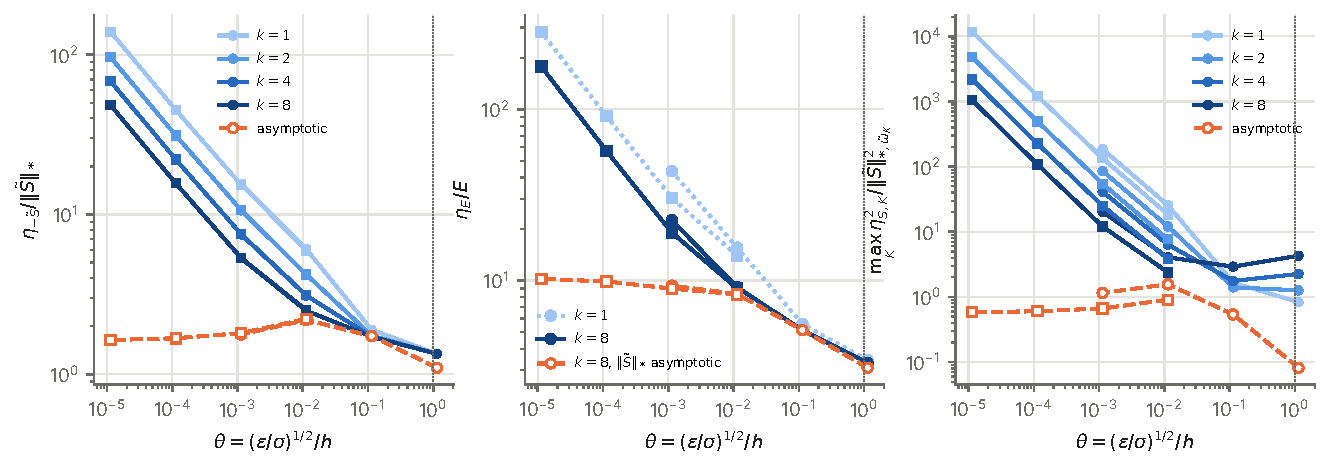
\includegraphics[width=\textwidth]{figures/sv_refref.pdf}
\caption{\asref{Reaction regime, layers problem, $n=16$, A+S estimator; circles $\sigma=1$, squares $\sigma=10^4$.
Left: $\eta_{-\Stil}/\|\Stil\|_*$ with $P_2$ references on $k$-times refined meshes and with the asymptotic value
\eqref{eq:Sasym}. Middle: $\eta_E/E$ with the same-mesh and the $8$ times refined references, and with
$\|\Stil\|_*$ from \eqref{eq:Sasym}. Right: the local ratio for $\ell=-\Stil$; the refined references are lower bounds
of the local dual norms, so these ratios are upper estimates; the asymptotic value is valid only for $\theta\ll1$.}}
\label{fig:refref}
\end{figure}

\begin{figure}[!htbp]
\centering
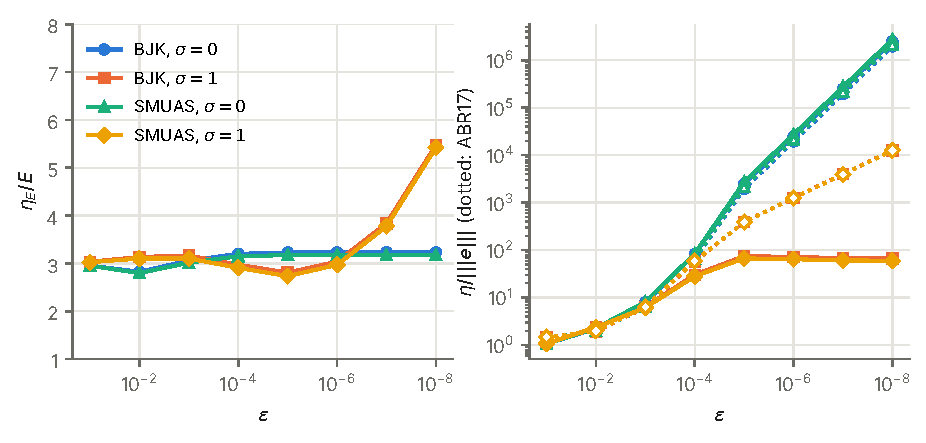
\includegraphics[width=\textwidth]{figures/sv_sweep.pdf}
\caption{Layers problem, $n=32$, as functions of $\eps$. Left: $I_E=\eta_E/E$. Right: the energy-norm
indices $\eta/\tnorm{e}$ (solid) and, dotted with open markers, that of the guaranteed bound of
\cite{ABR17}.}
\label{fig:sweep}
\end{figure}

\subsection{Variable reaction}\label{sec:num-cb}

With $c=1+(c_{\max}-1)xy$ and $\sigma=1$, the constant of (H3) is $\|c\|_\infty/\sigma=c_{\max}$, attained at
the vertex $(1,1)$. \refe{The computed $c_b$ is the sampled enclosure of Remark~\ref{rem:CF}, which is diagnostic: $c$ is not
affine on the cells, so the sampled maximum is enlarged by $\frac{h_K}2\max|\nabla c|$; here this gives} $c_b=1.12\,c_{\max}$, $1.06\,c_{\max}$
and $1.03\,c_{\max}$ for $n=8,16,32$, and $\kappa=2+c_b$ (Table~\ref{tab:cb}). The bound $E\le\eta_E$ holds in
all runs. The index of $\eta_{E,c}$ grows at most linearly, $\eta_{E,c}/E_c\le3\,c_b$ in all runs, as
Corollary~\ref{cor:twoc} predicts; it is often much smaller, down to $0.05\,c_b$, because the factor $M=c_b$ in front of $\tnorm{e}$ in $E_c$ also enlarges the
error measure. The index of $\eta_E$ grows faster, up to $5.2\,c_b$ at $c_b\approx10^3$, but stays far
below the worst case $(1+c_b)^2$ of Corollary~\ref{cor:two}. A variable reaction with a small lower
bound $\sigma$ is therefore the one situation in which the estimator loses its robustness, in
accordance with the theory; Section~\ref{sec:concl} discusses how to remove it.

% generated by examples/convection_diffusion/sv_numerics/make_figures.py; do not edit
\begin{table}[!htbp]
\centering
\small
\setlength{\tabcolsep}{4pt}
\caption{Variable reaction $c=1+(c_{\max}-1)xy$, $\sigma=1$, $\eps\in\{10^{-3},10^{-6}\}$, $n\in\{8,16,32\}$: ranges over the six runs; $c_b$ and $\kappa$ are the means of the sampled enclosures (Remark~\ref{rem:CF}; diagnostic), which exceed $c_{\max}$ by $3$--$12\,\%$.}\label{tab:cb}
\begin{tabular}{rrrllll}
\toprule
$c_{\max}$ & $c_b$ & $\kappa$ & $\eta_E/E$ & $\eta_{E,c}/E_c$ & $\eta_{E,c}/(c_bE_c)$ & $E\le\eta_E$\\
\midrule
1 & 1.00 & 3.00 & 3.85--5.34 & 3.85--5.34 & 3.85--5.34 & yes\\
10 & 10.66 & 12.66 & 14.63--19.94 & 8.69--30.35 & 0.85--2.95 & yes\\
100 & 107.22 & 109.22 & 128--271 & 12.27--216 & 0.12--2.09 & yes\\
1000 & $1.1\cdot10^{3}$ & $1.1\cdot10^{3}$ & 1618--5312 & 56.23--1125 & 0.05--1.09 & yes\\
\bottomrule
\end{tabular}
\end{table}


\subsection{Local efficiency}\label{sec:num-loc}

Table~\ref{tab:loc} reports the localised measure for the layers problem on the $16\times16$ mesh. The
local ratio $\max_K\eta_K^2/E_{\mathrm{loc}}(\tilde\omega_K)^2$ is at most $0.51$ in all cases, and
independent of $\eps$ for $\eps\le10^{-4}$: the estimator is locally efficient, as stated in
Theorem~\ref{thm:loc}. The ratio $E_{\mathrm{loc}}/E$ lies between $0.48$ and $1.01$, so on these
problems the localised measure captures most of the global one, and the guaranteed bound
$E_{\mathrm{loc}}\le\sqrt{d+1}\,\eta_E$ of Theorem~\ref{thm:loc} overestimates $E_{\mathrm{loc}}$ by a
factor $5$--$12$. The largest value, $\eta_E/E_{\mathrm{loc}}=7.0$ for $\sigma=1$ and $\eps=10^{-8}$, is the
same reference effect as in Section~\ref{sec:num-robust}.

% generated by examples/convection_diffusion/sv_numerics/make_figures.py; do not edit
\begin{table}[!htbp]
\centering
\small
\setlength{\tabcolsep}{4pt}
\caption{Localised measure (Theorem~\ref{thm:loc}), outflow layers, BJK, $n=16$. The last but one column is $\max_K\eta_K^2/E_{\mathrm{loc}}(\tilde\omega_K)^2$ with $\eta_K=\eta_{A,K}+\eta_{S,K}$.}\label{tab:loc}
\begin{tabular}{rrrrrrr}
\toprule
$\sigma$ & $\eps$ & $E_{\mathrm{loc}}/E$ & $\eta_E/E_{\mathrm{loc}}$ & $\sqrt{d+1}\,\eta_E/E_{\mathrm{loc}}$ & local max & $I_E$\\
\midrule
0 & $10^{-2}$ & 0.48 & 5.94 & 10.29 & 0.26 & 2.88\\
0 & $10^{-4}$ & 0.60 & 5.50 & 9.53 & 0.37 & 3.28\\
0 & $10^{-6}$ & 0.60 & 5.50 & 9.52 & 0.37 & 3.29\\
0 & $10^{-8}$ & 0.60 & 5.50 & 9.52 & 0.37 & 3.29\\
1 & $10^{-2}$ & 0.52 & 6.38 & 11.05 & 0.51 & 3.33\\
1 & $10^{-4}$ & 0.95 & 3.07 & 5.32 & 0.13 & 2.93\\
1 & $10^{-6}$ & 1.01 & 3.47 & 6.01 & 0.07 & 3.51\\
1 & $10^{-8}$ & 1.01 & 7.04 & 12.20 & 0.07 & 7.13\\
\bottomrule
\end{tabular}
\end{table}


\subsection{Adaptive refinement}\label{sec:num-adapt}

Starting from the $8\times8$ mesh, we mark by the indicators $\eta_K=\eta_{A,K}+\eta_{S,K}$ with the
dual strategy of \cite{AJ27} (all cells with $\eta_K\ge\theta\max\eta$, $\theta=0.5$, reduced until at least
$5\,\%$ of the cells are marked) and refine by red--green refinement, until $N>3\cdot10^4$.
Table~\ref{tab:adapt} and Figures~\ref{fig:adapt} and~\ref{fig:adaptmesh} show the results for the layers
problem.
\begin{itemize}
  \item \textbf{Effectivity.} $I_E$ stays between $2.86$ and $3.55$ in every loop of all three runs, from
  $N=81$ to $N=45\,094$, while the local mesh size spans three orders of magnitude.
  \item \textbf{Where the mesh is refined.} The refinement concentrates in the outflow layers at $x=1$ and
  $y=1$ (Figure~\ref{fig:adaptmesh}); the smallest cells have $h_{\min}=3.5\cdot10^{-4}$ for $\eps=10^{-3}$,
  below $\eps$, so the layers are resolved, and $h_{\min}=1.7\cdot10^{-4}$ for $\eps=10^{-5}$, where they are not.
  \item \textbf{Convergence.} For $\eps=10^{-3}$, $E$ decreases at the rate $1.8$--$1.9$ with respect to
  $N^{-1/2}$ over the second half of the loops: this is the pre-asymptotic phase in which the layers become
  resolved, faster than the optimal rate $1$. For $\eps=10^{-5}$ the rate is $0.98$. On the finest uniform mesh
  ($N=16\,641$) the error $E$ is $18$, $4.4$ and $17$ times larger than the adaptive error at the same $N$.
  Under uniform refinement $E$ decreases at the rate $0.46$--$0.60$ for $\sigma=0$ and $0.04$--$0.51$ for
  $\sigma=1$, because the layers are never resolved; the index $I_E$ is $2.86$--$3.37$ there as well.
  \item \textbf{Energy norm.} Along the adaptive runs the energy-norm index $I$ falls from $29$ to $1.1$
  ($\eps=10^{-3}$) and from $8.4\cdot10^3$ to $6.2$ ($\eps=10^{-5}$): once the mesh resolves the layers, the
  energy error and the dual norm of the residual become comparable, while $I_E$ is insensitive to this.
\end{itemize}

% generated by examples/convection_diffusion/sv_numerics/make_figures.py; do not edit
\begin{table}[!htbp]
\centering
\small
\setlength{\tabcolsep}{4pt}
\caption{Adaptive refinement for the outflow-layers problem, BJK, dual marking by the SV indicators $\eta_K$, red--green refinement. The rate is that of $E$ with respect to $N^{-1/2}$ over the second half of the loops; the last column is the ratio of $E$ on the finest uniform mesh ($N=16641$) to the adaptive $E$ at the same $N$.}\label{tab:adapt}
\begin{tabular}{rrrrllrlr}
\toprule
$\eps$ & $\sigma$ & loops & $N$ (last) & $h_{\min}$ & $E$ (last) & rate & $\eta_E/E$ & gain\\
\midrule
$10^{-3}$ & 0 & 15 & 33010 & $3.45\cdot10^{-4}$ & $7.395\cdot10^{-2}$ & 1.88 & 2.86--3.25 & 18.3\\
$10^{-5}$ & 0 & 12 & 31866 & $1.73\cdot10^{-4}$ & $3.941$ & 0.98 & 2.94--3.35 & 4.4\\
$10^{-3}$ & 1 & 17 & 45094 & $1.73\cdot10^{-4}$ & $5.891\cdot10^{-2}$ & 1.83 & 2.96--3.55 & 17.2\\
\bottomrule
\end{tabular}
\end{table}


\begin{figure}[!htbp]
\centering
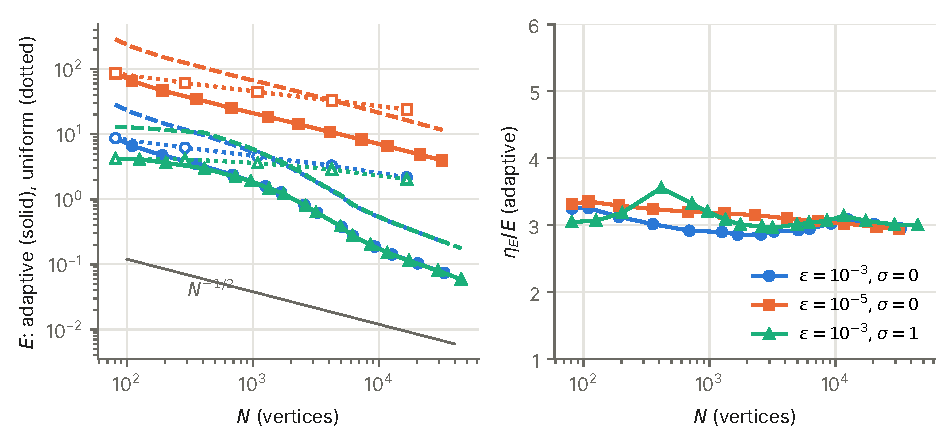
\includegraphics[width=\textwidth]{figures/sv_adapt.pdf}
\caption{Adaptive refinement, layers problem, BJK. Left: $E$ for adaptive (solid) and uniform (dotted, open
markers) refinement, and $\eta_E$ for the adaptive runs (dashed). Right: $I_E$ along the adaptive runs.}
\label{fig:adapt}
\end{figure}

\begin{figure}[!htbp]
\centering
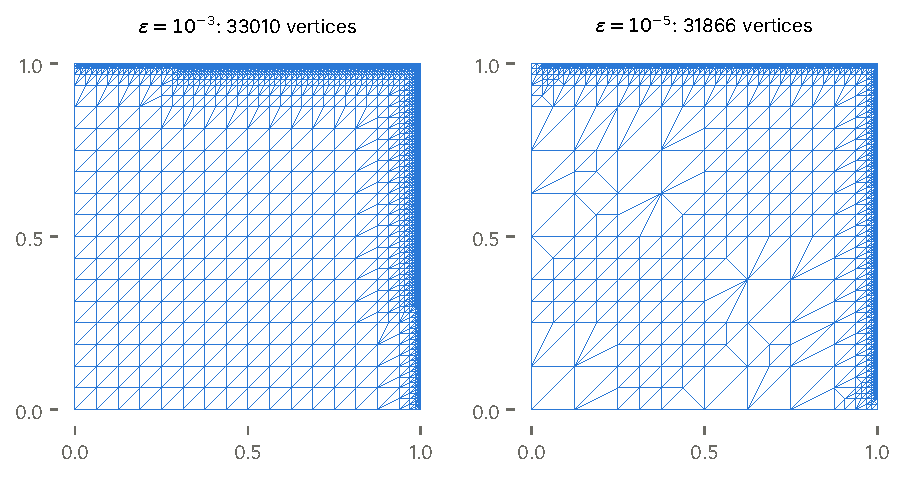
\includegraphics[width=\textwidth]{figures/sv_adapt_mesh.pdf}
\caption{Final adaptive meshes, layers problem, $\sigma=0$.}
\label{fig:adaptmesh}
\end{figure}

\subsection{\adapt{Uniform versus adaptive refinement}}\label{sec:num-unad}
{\color{magenta}

We repeat the uniform-mesh studies of Tables~\ref{tab:conv} and~\ref{tab:sweep} with adaptive refinement:
the same problems, the same marking as in Section~\ref{sec:num-adapt}, from the $8\times8$ mesh up to
$N\approx2\cdot10^4$ (Table~\ref{tab:conv}) and $N\approx10^4$ (Table~\ref{tab:sweep}). For the robustness
sweep we compare at equal cost: the adaptive loop whose $N$ is closest to $N=1089$, the size of the $32\times32$
mesh of Table~\ref{tab:sweep}.

\paragraph{Refinement studies (Figure~\ref{fig:aconv}).}
\begin{itemize}
  \item \textbf{Effectivity.} Along the adaptive runs $I_E$ lies in $2.83$--$4.18$ and tends to the same values
  as on uniform meshes, about $3.0$--$3.2$. The bound held in every loop.
  \item \textbf{Accuracy.} For the smooth solution, adaptive refinement gains nothing: at $N=16\,641$ the two
  errors agree to within $1\,\%$, and $E$ converges at the rate $1$ in both cases. For the layers problem the
  uniform error is $5.4$ ($\eps=10^{-2}$) and $5.9$ ($\eps=10^{-4}$) times the adaptive one at the same $N$.
  For $\eps=10^{-4}$, $E$ converges at the rate $0.47$ under uniform refinement and at $1.4$--$1.9$ in the last
  adaptive loops, in which the layers become resolved.
\end{itemize}

\begin{figure}[!htbp]
\centering
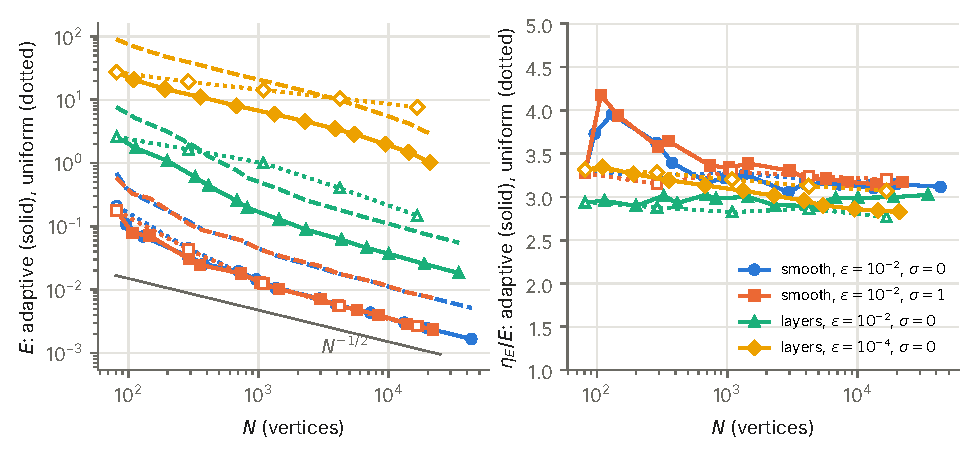
\includegraphics[width=\textwidth]{figures/sv_aconv.pdf}
\caption{\adapt{The cases of Table~\ref{tab:conv} under adaptive refinement. Left: $E$ for adaptive (solid) and uniform
(dotted, open markers) refinement, and $\eta_E$ for the adaptive runs (dashed). Right: $I_E$, adaptive (solid) and
uniform (dotted).}}
\label{fig:aconv}
\end{figure}

\paragraph{Robustness sweep (Figures~\ref{fig:abudget} and~\ref{fig:aloops}).}
\begin{itemize}
  \item \textbf{$\sigma=0$.} At equal cost, $I_E=2.89$--$3.22$ on the adaptive meshes against $2.80$--$3.23$ on the
  uniform mesh, for all $\eps$ and both stabilisations, and it stays in $2.82$--$3.35$ over all loops: the
  estimator is as robust on the meshes it generates as on the fixed mesh.
  \item \textbf{$\sigma=1$, small $\eps$.} The rise of $I_E$ to $5.4$--$5.5$ on the uniform mesh at
  $\eps\le10^{-7}$ (Section~\ref{sec:num-robust}) does not occur at equal cost on the adaptive meshes, where
  $I_E=2.75$--$3.16$. Figure~\ref{fig:aloops} shows why. The large values, up to $9.6$, appear only on the
  coarse initial mesh, and they come from the stabilisation part: $I_S=17.8$ at $N=81$ for $\eps=10^{-8}$. As the
  mesh resolves the layers, $I_S$ falls to $1.5$--$1.6$ and $I_E$ returns to about $3$. This confirms that the
  rise on the uniform mesh is a property of the under-resolved $P_2$ reference for $\|\Stil\|_*$, not of the
  estimator.
  \item \textbf{Smooth problem.} For $\eps\le10^{-3}$ the adaptive indices are higher than the uniform ones at
  equal cost: $I_E=4.0$--$5.3$ against $3.6$--$3.8$ for $\sigma=0$, and $4.5$--$6.0$ against $3.9$--$6.0$ for
  $\sigma=1$. Along the runs they reach $7.8$ after the first loop, and $10.9$ on the initial mesh. For $\sigma=1$
  and $\eps\le10^{-6}$ the fixed-point iteration reaches the iteration limit $2\cdot10^4$ on most meshes beyond
  $N\approx1100$, and the bound holds at these iterates.
  \item \textbf{Energy norm.} At $\sigma=0$ the energy-norm index still grows like $\eps^{-1}$ on the adaptive meshes,
  to $4\cdot10^5$ at $\eps=10^{-8}$ (uniform: $2.5\cdot10^6$); only the augmented measure is robust.
  \item \textbf{An open point.} For the layers problem with $\sigma=1$ and $\eps=10^{-6}$, $I_E$ rises again in the
  last loops, from $2.8$ to $4.3$, together with $I_\oplus$ (from $3.2$ to $6.6$). We have not identified the cause;
  it may be the convective part of the reference becoming resolved, and would need runs beyond $N=10^4$.
\end{itemize}

\begin{figure}[!htbp]
\centering
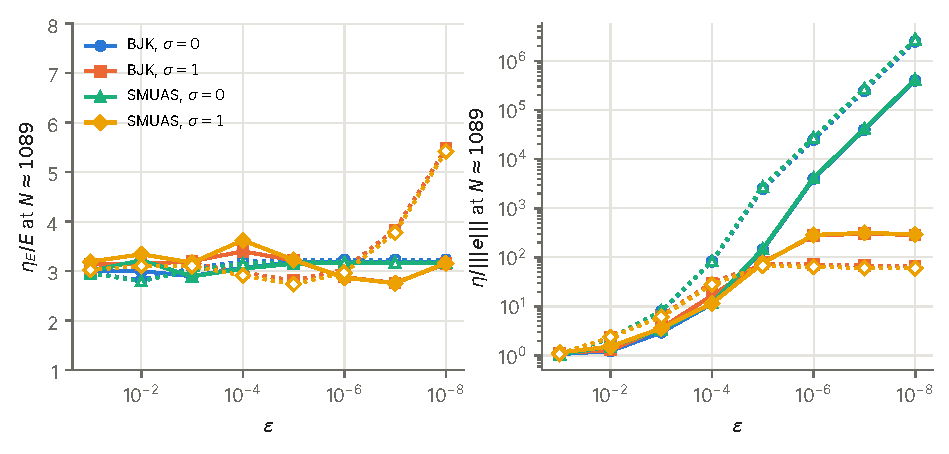
\includegraphics[width=\textwidth]{figures/sv_asweep_budget.pdf}
\caption{\adapt{The robustness sweep of Table~\ref{tab:sweep} at equal cost, layers problem: adaptive meshes with
$N\approx1089$ (solid) against the uniform $32\times32$ mesh (dotted, open markers). Left: $I_E$. Right: the
energy-norm index $\eta/\tnorm{e}$.}}
\label{fig:abudget}
\end{figure}

\begin{figure}[!htbp]
\centering
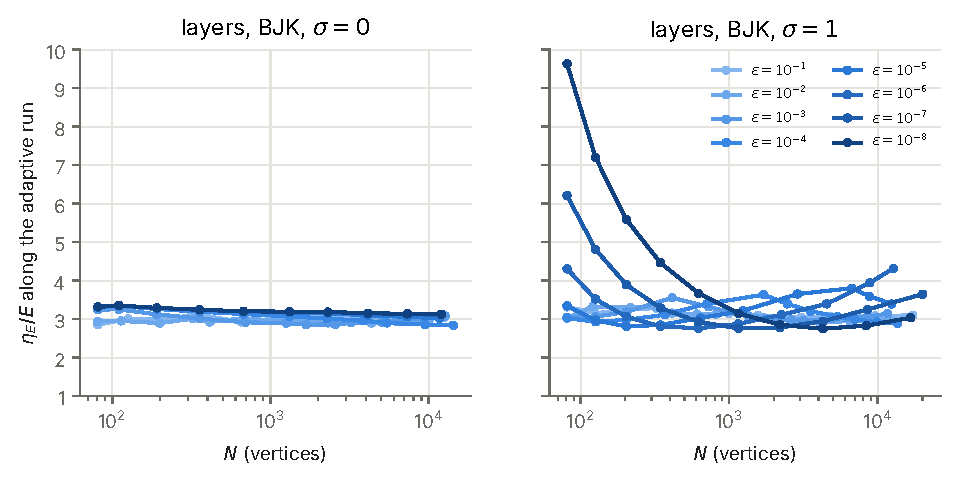
\includegraphics[width=\textwidth]{figures/sv_asweep_loops.pdf}
\caption{\adapt{$I_E$ along the adaptive runs of the robustness sweep, layers problem, BJK; one line per $\eps$, darker for
smaller $\eps$.}}
\label{fig:aloops}
\end{figure}

\paragraph{Which refinement to use.} For computing solutions, adaptive refinement is clearly preferable when the
solution has layers, by factors $4$--$18$ in $E$ at equal $N$, and it is what the estimator is designed for. For
testing the theory, the uniform meshes remain the primary evidence: a fixed coarse mesh keeps the layers
unresolved, which is the regime in which robustness can fail, isolates the dependence on $\eps$ and $\sigma$, and
is the only setting in which rates in $h$ are meaningful. The adaptive runs confirm that the effectivity stays at
about $3$ on the meshes the estimator generates itself.
}% end of the magenta block

\subsection{Inexact iterates and adaptive stopping}\label{sec:num-stop}

\paragraph{Iterates.} Table~\ref{tab:iter} and Figure~\ref{fig:iter} evaluate the estimator at the
fixed-point iterates $u^i$ on the $16\times16$ mesh. The index $I_E$ stays between $2.9$ and $5.3$ at
every iterate, including the first one, where the algebraic part $\eta_{\mathrm{alg}}$ is up to $71\,\%$
of $\eta_{\mathrm{disc}}$: this is part~2 of Proposition~\ref{prop:stop}, efficiency at every iterate
without any condition on the algebraic error. The ratio $\eta_{\mathrm{alg}}/\eta_{\mathrm{disc}}$
decreases monotonically for all problems except the smooth one with $\eps=10^{-6}$ and $\sigma=0$, for
which the fixed-point iteration does not converge in $2\cdot10^4$ iterations; there the ratio stalls
between $10^{-3}$ and $4\cdot10^{-3}$. In that case the error is smallest at $i\approx10$, $E(u^{10})=4.8$, and grows to
$8.4$ at $i=2\cdot10^4$: further iterations make the iterate worse in $E$, and the estimator, which is
efficient at every iterate, reflects this.

% generated by examples/convection_diffusion/sv_numerics/make_figures.py; do not edit
\begin{table}[!htbp]
\centering
\small
\setlength{\tabcolsep}{4pt}
\caption{Fixed-point iterates $u^i$, $i\in\{1,2,5,\dots,1000\}$ below the converged count, and the converged solution; BJK, $n=16$. The split is $\eta_{\mathrm{disc}}=\eta_E-\eta_{\mathrm{alg}}$.}\label{tab:iter}
\begin{tabular}{lrrrlrrl}
\toprule
problem & $\eps$ & $\sigma$ & it.\ to tol. & $\eta_E/E$ over $i$ & $\max_i\eta_{\mathrm{alg}}/\eta_{\mathrm{disc}}$ & $E(u^1)/E(u^{\mathrm{last}})$ & $E\le\eta_E$\\
\midrule
smooth & $10^{-2}$ & 0 & 39 & 3.24--3.63 & 0.71 & 1.81 & yes\\
smooth & $10^{-2}$ & 1 & 37 & 3.15--3.45 & 0.51 & 1.58 & yes\\
smooth & $10^{-6}$ & 0 & 20000 & 3.76--4.61 & 0.58 & 1.06 & yes\\
smooth & $10^{-6}$ & 1 & 664 & 4.42--5.28 & 0.19 & 1.20 & yes\\
layers & $10^{-2}$ & 0 & 47 & 2.88--2.97 & 0.02 & 1.01 & yes\\
layers & $10^{-2}$ & 1 & 45 & 3.32--3.33 & 0.01 & 1.01 & yes\\
layers & $10^{-6}$ & 0 & 635 & 3.29--3.47 & 0.04 & 1.01 & yes\\
layers & $10^{-6}$ & 1 & 502 & 3.51--3.56 & 0.02 & 1.03 & yes\\
\bottomrule
\end{tabular}
\end{table}


\begin{figure}[!htbp]
\centering
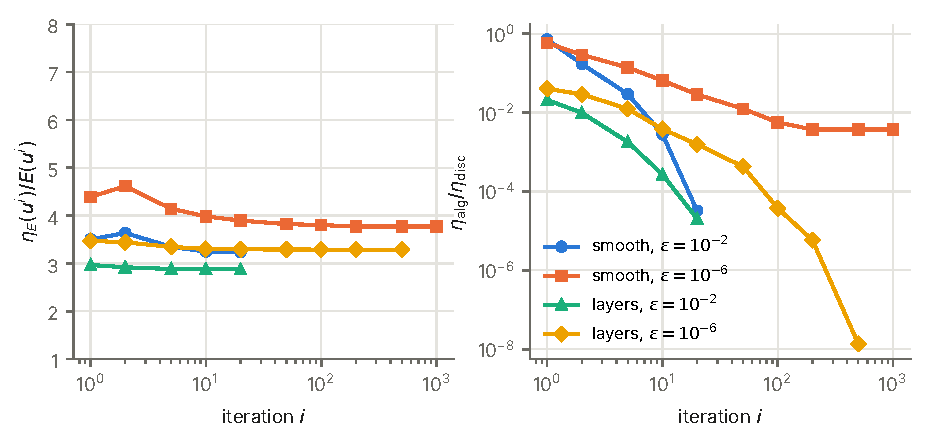
\includegraphics[width=\textwidth]{figures/sv_iter.pdf}
\caption{Fixed-point iterates, BJK, $\sigma=0$, $n=16$. Left: $I_E$ at the iterate $u^i$. Right: the
ratio $\eta_{\mathrm{alg}}/\eta_{\mathrm{disc}}$ (points with a ratio below $10^{-8}$ are omitted).}
\label{fig:iter}
\end{figure}

\paragraph{Adaptive stopping.} Table~\ref{tab:stop} runs five adaptive loops \refe{as in} Section~\ref{sec:num-adapt}
in which the fixed-point iteration is stopped either at the fixed tolerance $\|r\|\le10^{-10}\sqrt N$ or by
the criterion \eqref{eq:stop}, $\eta_{\mathrm{alg}}\le\gamma\eta_{\mathrm{disc}}$, with
$\eta_{\mathrm{disc}}=\eta_E-\eta_{\mathrm{alg}}$; each loop starts from the zero initial guess.
\begin{itemize}
  \item \textbf{Savings.} With $\gamma=0.1$, the total number of iterations drops from $227$ to $25$ (smooth,
  $\eps=10^{-2}$) and from $2323$ to $25$ (layers, $\eps=10^{-4}$), by factors $9$ and $93$; with $\gamma=0.01$
  the factors are $4.5$ and $46$.
  \item \textbf{Accuracy.} The final error $E$ changes by at most $6\,\%$ ($\gamma=0.1$, layers) and by at most
  $0.3\,\%$ for $\gamma\le0.01$. The index $I_E$ stays in $3.1$--$4.8$ in all runs, and in every stopped loop
  $\eta_{\mathrm{alg}}/\eta_{\mathrm{disc}}\le\gamma$, so $E\le(1+\gamma)\eta_{\mathrm{disc}}$
  (Proposition~\ref{prop:stop}, part~3).
  \item \textbf{Non-converging iteration.} For the smooth problem with $\eps=10^{-6}$ the fixed-point
  iteration does not reach the tolerance within $10^4$ iterations on any mesh, and $50\,000$ iterations give
  $E=3.22$. The criterion with $\gamma=0.1$ stops after $5$--$15$ iterations per loop, $50$ in total, with a
  \emph{smaller} error, $E=1.98$: as in Figure~\ref{fig:iter}, the early iterates are better than the late
  ones. For $\gamma=10^{-3}$ the criterion fires in only one of the five loops, since $\eta_{\mathrm{alg}}/\eta_{\mathrm{disc}}$ stalls
  at about $3\cdot10^{-3}$; this is a property of the iteration, not of the estimator.
\end{itemize}

% generated by examples/convection_diffusion/sv_numerics/make_figures.py; do not edit
\begin{table}[!htbp]
\centering
\footnotesize
\setlength{\tabcolsep}{4pt}
\caption{Adaptive stopping in five adaptive loops (dual marking by the SV indicators, red--green refinement), BJK, $\sigma=0$. ``tol.'' is the fixed tolerance $\|r\|\le10^{-10}\sqrt N$; otherwise the iteration stops at $\eta_{\mathrm{alg}}\le\gamma\eta_{\mathrm{disc}}$ (at most $10^4$ iterations). The last column says whether every loop stopped before the iteration limit.}\label{tab:stop}
\begin{tabular}{lrrrrlllr}
\toprule
problem & $\eps$ & $\gamma$ & it./loop & total & $E$ (last) & $\eta_E/E$ & $\max\eta_{\mathrm{alg}}/\eta_{\mathrm{disc}}$ & stopped\\
\midrule
smooth & $10^{-2}$ & tol. & 30--59 & 227 & $2.550\cdot10^{-2}$ & 3.29--3.95 & $5.78\cdot10^{-8}$ & yes\\
smooth & $10^{-2}$ & 0.1 & 5 & 25 & $2.554\cdot10^{-2}$ & 3.41--3.97 & $5.07\cdot10^{-2}$ & yes\\
smooth & $10^{-2}$ & 0.01 & 10 & 50 & $2.551\cdot10^{-2}$ & 3.33--3.98 & $7.27\cdot10^{-3}$ & yes\\
smooth & $10^{-2}$ & 0.001 & 10--20 & 80 & $2.551\cdot10^{-2}$ & 3.29--3.96 & $9.89\cdot10^{-4}$ & yes\\
smooth & $10^{-6}$ & tol. & 10000 & 50000 & $3.218$ & 3.77--4.58 & $3.03\cdot10^{-3}$ & no\\
smooth & $10^{-6}$ & 0.1 & 5--15 & 50 & $1.984$ & 4.04--4.79 & $9.83\cdot10^{-2}$ & yes\\
smooth & $10^{-6}$ & 0.01 & 120--760 & 2190 & $2.749$ & 3.80--4.45 & $9.10\cdot10^{-3}$ & yes\\
smooth & $10^{-6}$ & 0.001 & 7320--10000 & 47320 & $3.218$ & 3.77--4.58 & $3.03\cdot10^{-3}$ & no\\
layers & $10^{-4}$ & tol. & 385--628 & 2323 & $8.044$ & 3.13--3.34 & $3.57\cdot10^{-9}$ & yes\\
layers & $10^{-4}$ & 0.1 & 5 & 25 & $8.524$ & 3.20--3.42 & $2.49\cdot10^{-2}$ & yes\\
layers & $10^{-4}$ & 0.01 & 10 & 50 & $8.023$ & 3.15--3.38 & $8.43\cdot10^{-3}$ & yes\\
layers & $10^{-4}$ & 0.001 & 25--50 & 175 & $8.04$ & 3.14--3.35 & $9.29\cdot10^{-4}$ & yes\\
\bottomrule
\end{tabular}
\end{table}


\subsection{Variable diffusion}\label{sec:num-vareps}

Table~\ref{tab:vareps} reports the variable-diffusion problems on the meshes $n=8,16,32$. All bounds are
guaranteed. For the smooth coefficient, the oscillation $\eta_\eps$ converges at the rate $2.09$--$2.13$
in $h$, in accordance with Lemma~\ref{lem:V}(iii), and is at most $12\,\%$ of $\eta$ (at contrast $10^4$ on
the coarsest mesh). For the jump aligned with the mesh, $\Pi_1\eps=\eps$ and $\eta_\eps=0$. The
effectivity $I_E$ lies in $2.6$--$4.5$ for contrasts up to $10^4$, for $\eps=10^{-2}$ and $10^{-6}$ alike. For
the jump it does not grow with the contrast; for the smooth coefficient it grows mildly, from
$3.1$ at contrast $1$ to at most $4.3$ at contrast $10^4$ (on the coarsest mesh). This is the quasi-monotone case; the constants of
Theorem~\ref{thm:vareps} depend on the patch contrast, but for an aligned jump that contrast does not
show up in the indices. Checkerboard (non-quasi-monotone) coefficients are not tested; for them no
local estimator can be robust \cite{Li26}.

% generated by examples/convection_diffusion/sv_numerics/make_figures.py; do not edit
\begin{table}[!htbp]
\centering
\footnotesize
\setlength{\tabcolsep}{4pt}
\caption{Variable diffusion, BJK, $\sigma=0$, $n\in\{8,16,32\}$: ranges over the three meshes. The rate is that of $\eta_\eps$ with respect to $N^{-1/2}$ between $n=16$ and $n=32$ (expected: $2$).}\label{tab:vareps}
\begin{tabular}{lrrllllrl}
\toprule
$\eps(x)$ & $\eps$ & contrast & $I$ & $I_\oplus$ & $I_E$ & $\max\eta_\eps/\eta$ & rate & $E\le\eta_E$\\
\midrule
smooth & $10^{-2}$ & 1 & 1.23--4.58 & 3.30--4.06 & 3.07--3.13 & 0.000 & --- & yes\\
smooth & $10^{-2}$ & 100 & 1.07--1.24 & 3.16--3.39 & 3.15--3.26 & 0.035 & 2.09 & yes\\
smooth & $10^{-2}$ & 10000 & 1.10--1.44 & 3.30--4.28 & 3.29--4.27 & 0.117 & 2.09 & yes\\
smooth & $10^{-6}$ & 1 & 7959--36796 & 3.72--5.01 & 3.50--3.70 & 0.000 & --- & yes\\
smooth & $10^{-6}$ & 100 & 818--3354 & 3.73--5.44 & 3.54--4.03 & 0.000 & 2.13 & yes\\
smooth & $10^{-6}$ & 10000 & 64.07--336 & 4.31--5.49 & 3.94--4.46 & 0.001 & 2.10 & yes\\
jump & $10^{-2}$ & 100 & 2.56--7.63 & 3.43--4.18 & 2.61--2.99 & 0.000 & --- & yes\\
jump & $10^{-2}$ & 10000 & 2.61--8.12 & 3.43--4.22 & 2.60--3.01 & 0.000 & --- & yes\\
jump & $10^{-6}$ & 100 & 9025--28125 & 4.75--5.12 & 3.44--3.54 & 0.000 & --- & yes\\
jump & $10^{-6}$ & 10000 & 2156--4989 & 4.78--5.08 & 3.41--3.52 & 0.000 & --- & yes\\
\bottomrule
\end{tabular}
\end{table}


\subsection{Three dimensions}\label{sec:num-3d}

Table~\ref{tab:d3} repeats the uniform-refinement study on the unit cube ($n=4,8,16$, up to $N=4913$
vertices and $24\,576$ tetrahedra).
\begin{itemize}
  \item \textbf{Layers.} $I_E=2.94$--$3.55$ for $\eps=10^{-2}$ and $10^{-6}$, as in two dimensions; $I_\oplus\le4.9$
  and $I_S=1.21$--$1.26$.
  \item \textbf{Smooth solution.} $I_E$ is higher than in two dimensions, $5.1$--$6.4$, but decreases under
  refinement for both values of $\eps$ ($5.97\to5.40$ and $6.39\to5.09$). These meshes are coarse: $E$ still
  converges at the pre-asymptotic rates $2.1$--$2.7$ in $h$, dominated by the stabilisation part
  $\|\Stil\|_*$, which is estimated sharply ($I_S=1.28$--$1.31$); the larger index comes from the convective
  dual norm on coarse tetrahedral meshes. For $\eps=10^{-6}$ on the finest mesh the fixed-point iteration does
  not converge within $2\cdot10^4$ iterations, and the bound still holds at the last iterate.
  \item \textbf{Energy norm.} As in two dimensions, $I$ is useless for $\sigma=0$ and small $\eps$
  ($1.0\cdot10^4$--$1.4\cdot10^5$ at $\eps=10^{-6}$, against $2.6$--$9.3$ at $\eps=10^{-2}$), while $I_E$ is not
  affected.
  \item \textbf{Cost.} The estimator takes about $8$\,s at $N=729$ and $220$--$240$\,s at $N=4913$ in our
  Python implementation; the cost is dominated by the vertex-patch problems in $\RTN$, whose size grows
  quickly with the number of tetrahedra per patch in three dimensions. The patch problems are independent and
  can be solved in parallel; the global $\RT_0$ defect problem takes a small fraction of the time.
\end{itemize}

% generated by examples/convection_diffusion/sv_numerics/make_figures.py; do not edit
\begin{table}[!htbp]
\centering
\small
\setlength{\tabcolsep}{4pt}
\caption{Three dimensions, uniform refinement of the unit cube, BJK, $\sigma=0$. Rates with respect to $N^{-1/3}\sim h$; the last column is the time of the estimator in seconds.}\label{tab:d3}
\begin{tabular}{lrrlrrrrr}
\toprule
problem & $\eps$ & $N$ & $E$ & rate & $I$ & $I_\oplus$ & $I_E$ & time\\
\midrule
smooth & $10^{-2}$ & 125 & $0.7$ &  & 9.27 & 7.82 & 5.97 & 0.7\\
smooth & $10^{-2}$ & 729 & $0.144$ & 2.69 & 4.83 & 6.98 & 5.71 & 9.0\\
smooth & $10^{-2}$ & 4913 & $3.55\cdot10^{-2}$ & 2.20 & 2.64 & 5.84 & 5.40 & 226.6\\
smooth & $10^{-6}$ & 125 & $6.72\cdot10^{1}$ &  & $7.4\cdot10^{4}$ & 9.26 & 6.39 & 0.6\\
smooth & $10^{-6}$ & 729 & $2.00\cdot10^{1}$ & 2.06 & $2.8\cdot10^{4}$ & 6.93 & 5.31 & 8.4\\
smooth & $10^{-6}$ & 4913 & $4.06$ & 2.51 & $1.0\cdot10^{4}$ & 5.56 & 5.09 & 238.0\\
layers & $10^{-2}$ & 125 & $2.74$ &  & 6.67 & 4.01 & 3.10 & 0.6\\
layers & $10^{-2}$ & 729 & $1.82$ & 0.70 & 4.31 & 3.71 & 3.01 & 8.0\\
layers & $10^{-2}$ & 4913 & $1.14$ & 0.73 & 2.93 & 3.64 & 2.94 & 217.3\\
layers & $10^{-6}$ & 125 & $2.79\cdot10^{2}$ &  & $1.4\cdot10^{5}$ & 4.71 & 3.38 & 0.5\\
layers & $10^{-6}$ & 729 & $2.01\cdot10^{2}$ & 0.56 & $7.3\cdot10^{4}$ & 4.78 & 3.47 & 8.5\\
layers & $10^{-6}$ & 4913 & $1.35\cdot10^{2}$ & 0.63 & $3.8\cdot10^{4}$ & 4.93 & 3.55 & 236.1\\
\bottomrule
\end{tabular}
\end{table}


\subsection{Summary}

The experiments answer the questions (Q1)--(Q7) as follows.
\begin{enumerate}[label=(Q\arabic*)]
  \item The bound $E\le\eta_E$ held in every run: two and three dimensions, both stabilisations,
  $\eps=10^{-1},\dots,10^{-8}$, $\sigma\in\{0,1\}$, variable reaction and diffusion, adaptive meshes and inexact
  iterates\refe{, and so did $I\ge1$, $I_\oplus\ge1$ and $I_S\ge1$. Since the references are lower bounds of the dual
  norms, this is a consistency check rather than a proof}.
  \item For constant coefficients, $I_E$ lies in $2.6$--$5.3$ in two dimensions, inexact iterates included,
  independently of $\eps$, $\sigma$, the stabilisation and the mesh; the only exception is a rise to $6.0$
  ($n=32$) and $7.1$ ($n=16$) at $\sigma=1$, $\eps\le10^{-7}$, \adapt{which the adaptive runs identify as an
  under-resolved reference for $\|\Stil\|_*$ (Section~\ref{sec:num-unad})}\asref{, as the asymptotically exact
  reference \eqref{eq:Sasym} confirms ($I_S=1.6$--$2.2$ and $\eta_E/E=8.3$--$10.2$ for $\theta$ down to $10^{-5}$)}; in three dimensions it is $2.9$--$6.4$ and
  decreases under refinement. The energy-norm index $I$, and the guaranteed bound of \cite{ABR17}, are not
  robust.
  \item The effectivity grows with $c_b$, at most linearly for $\eta_{E,c}$ and well below $c_b^2$ for $\eta_E$:
  a variable reaction with a small lower bound is the one case in which robustness is lost, as the theory
  predicts.
  \item The local ratio $\max_K\eta_K^2/E_{\mathrm{loc}}(\tilde\omega_K)^2$ is at most $0.51$.
  \item Adaptive refinement driven by $\eta_K$ resolves the layers and reduces $E$ by factors $4$--$18$
  against uniform refinement at equal $N$, with $I_E=2.9$--$3.6$ throughout. \adapt{Repeating the refinement and
  robustness studies adaptively gives the same effectivity, about $3$, as on uniform meshes.}
  \item The estimator is efficient at every iterate, and the stopping criterion saves up to $99\,\%$ of the
  iterations at a change of the error of at most $6\,\%$ ($\gamma=0.1$) or $0.3\,\%$ ($\gamma\le0.01$).
  \item For variable diffusion, $\eta_\eps$ converges at rate $2$ and $I_E$ stays in $2.6$--$4.5$ up to contrast
  $10^4$.
\end{enumerate}

\paragraph{Reproducibility.} All results are produced by the scripts \texttt{run\_numerics.py} and
\texttt{make\_figures.py} in the directory
\path{examples/convection_diffusion/sv_numerics} of \texttt{galerkit}. The first runs the experiments (about
$35$ minutes on four cores, the three-dimensional runs sequentially because of their memory use); the
second writes the tables, the figures and, for every stored solution, a VTK file
(\texttt{.vtu}) with $u_h$, $u$, $u-u_h$, $\eps$, $\eta_K$, $\tnorm{e}_K$ and the local effectivity
$\eta_K/\tnorm{e}_K$. \adapt{The figures of Section~\ref{sec:num-unad} are produced by
\texttt{make\_adaptive\_figures.py} in the same directory.}

).
% Data: examples/convection_diffusion/sv_numerics/run_numerics.py (output/*.json);
% tables and figures: make_figures.py -> tables/*.tex, figures/sv_*.{pdf,png}.
% All numbers quoted in the text below are read off those tables.

% ===========================================================================
\section{Numerical experiments}\label{sec:num}
% ===========================================================================

We test the estimator against the exact error. The questions are the ones raised by the theory:
\begin{enumerate}[label=(Q\arabic*)]
  \item Is the bound guaranteed, $E\le\eta_E$, in every run (Theorem~\ref{thm:rel})?
  \item Are the effectivity indices bounded independently of $\eps$, $\sigma$ and the stabilisation
  (Theorem~\ref{thm:eff}, Corollary~\ref{cor:two}), and do they stay bounded under refinement?
  \item Does the dependence on $c_b$ follow Corollaries~\ref{cor:two} and~\ref{cor:twoc}?
  \item Is the estimator locally efficient in the localisable measure (Theorem~\ref{thm:loc})?
  \item Do the indicators drive adaptive refinement to the optimal rate?
  \item Are the bounds valid at inexact iterates, and does the stopping criterion of
  Proposition~\ref{prop:stop} save iterations without spoiling the error?
  \item Does the variable-diffusion version keep its effectivity, with $\eta_\eps=O(h^2)$
  (Theorem~\ref{thm:vareps})?
\end{enumerate}

\subsection{Setup}

\paragraph{Discretisation.} Conforming $P_1$ elements on uniform meshes of the unit square
($n\times n$ squares, each cut into two triangles; $N=(n+1)^2$ vertices) or the unit cube ($n^3$
cubes, each cut into six tetrahedra), and on red--green refined meshes in the adaptive runs. The
stabilisations are the AFC scheme with the limiter of \cite{BJK17} (BJK), and the symmetrised
monotone upwind-type algebraic stabilisation of \cite{Kn23} (SMUAS). The nonlinear problem is solved
by the damped fixed-point iteration of \cite{AJ27} up to $\|r\|\le10^{-10}\sqrt N$, with at most
$2\cdot10^4$ iterations, unless stated otherwise.

\paragraph{Test problems} (all with $b$ constant, so $\sigma=c$, $c_b=1$ and $\kappa=3$, except in
Section~\ref{sec:num-cb}).
\begin{itemize}
  \item \emph{smooth}: $u=\prod_i\sin(\pi x_i)+x_1^2\prod_{i>1}x_i$, $b=(1,\tfrac12)$ or
  $(1,\tfrac12,\tfrac14)$, Dirichlet data on $\partial\Omega$; $f$ is computed from $u$. The solution
  has no layers, so its error is not dominated by layers, but for small $\eps$ the scheme is
  convection-dominated on every mesh used.
  \item \emph{layers}: $u=\prod_iw(x_i)$ with
  $w(s)=s-\bigl(e^{(s-1)/\eps}-e^{-1/\eps}\bigr)/\bigl(1-e^{-1/\eps}\bigr)$, $b=(1,\dots,1)$, homogeneous
  Dirichlet data; $u$ has exponential layers of width $\eps$ at the outflow boundary $x_i=1$.
  \item \emph{variable diffusion}: $u=\phi(x_1)\prod_{i>1}4x_i(1-x_i)$, either with
  $\eps(x)=\eps\,k^{x_1}$, $\phi(s)=4s(1-s)$ (\emph{smooth}), or with $\eps$ jumping from $\eps$ to $k\eps$
  at $x_1=\frac12$ and $\phi$ chosen such that the flux $\eps\phi'$ is continuous (\emph{jump}); $k$ is
  the contrast.
\end{itemize}

\paragraph{Error measures.} $\tnorm{e}$ is computed with a quadrature of degree~8. The dual norms
$\|B_A'(e,\cdot)\|_*$ and $\|\Stil\|_*$, and the local dual norms of $E_{\mathrm{loc}}$, are computed
from their Riesz representatives in the $P_2$ space on the same mesh (on each vertex patch for
$E_{\mathrm{loc}}$). These are \emph{lower} bounds of the true dual norms, so the reported effectivity
indices are slight overestimates; they become crude when the dual norm concentrates in layers that
the mesh does not resolve (see Section~\ref{sec:num-robust}). We report the effectivity indices
\[
  I=\frac{\eta}{\tnorm{e}},\qquad I_\oplus=\frac{\kappa\eta}{\tnorm{e}_\oplus},\qquad
  I_S=\frac{\eta_S}{\|\Stil\|_*},\qquad I_E=\frac{\eta_E}{E},
\]
of which $I_E$ is the one covered by Corollary~\ref{cor:two}; $I_\oplus\ge1$ and $I\ge1$ are guaranteed
too, but only $I_\oplus$ is expected to be robust.

\subsection{Solutions and indicators}

Figure~\ref{fig:snap} shows the discrete solution of the layers problem for $\eps=10^{-3}$ on the
$32\times32$ mesh, the cell indicators $\eta_K=\eta_{A,K}+\eta_{S,K}$, and the local energy errors
$\tnorm{e}_K$. The mesh does not resolve the layers ($h\approx4.4\cdot10^{-2}\gg\eps$); the AFC
solution is free of oscillations, and both the indicators and the error concentrate in the cells at
the outflow boundary, with a decay of several orders of magnitude into the interior. The indicator
is larger than $\tnorm{e}_K$ in the layer cells: it measures the residual in the dual norm, which
contains the convective part $\|B_A'(e,\cdot)\|_*$ of the error.

\begin{figure}[!htbp]
\centering
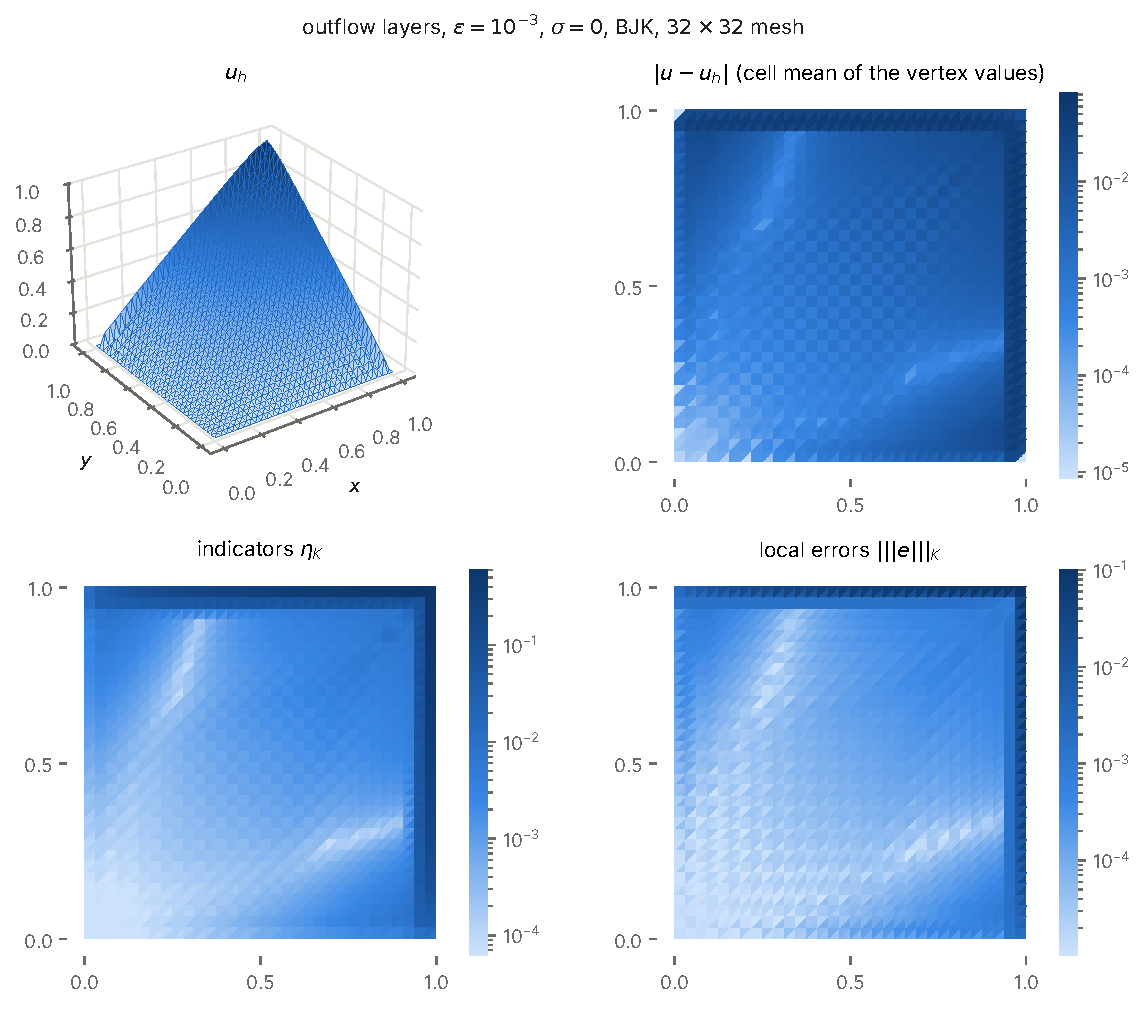
\includegraphics[width=\textwidth]{figures/sv_snap.pdf}
\caption{Layers problem, $\eps=10^{-3}$, $\sigma=0$, BJK, $n=32$: discrete solution $u_h$, indicators
$\eta_K$ and local errors $\tnorm{e}_K$ (logarithmic colour scale, common to both).}
\label{fig:snap}
\end{figure}

\subsection{Uniform refinement}\label{sec:num-conv}

Table~\ref{tab:conv} and Figure~\ref{fig:conv} report uniform refinement from $n=8$ to $n=128$.
\begin{itemize}
  \item \textbf{Smooth solution, $\eps=10^{-2}$.} $E$ and $\eta_E$ converge at the optimal rate $1$ in
  $h$ once the mesh resolves the solution; on the coarse meshes both decrease faster, because the
  stabilisation term $\|\Stil\|_*$ dominates $E$ there and decreases at a higher rate. The effectivity
  $I_E$ lies between $3.15$ and $3.29$ for $\sigma=0$ and $\sigma=1$ alike. The energy-norm index $I$
  tends to $1.1$: in the diffusion-dominated regime the energy norm and the dual norm of the
  residual coincide asymptotically.
  \item \textbf{Layers, $\eps=10^{-2}$.} The layers are resolved only from $n=64$ on, and the
  convergence of $E$ accelerates accordingly; $I_E$ stays between $2.77$ and $2.94$.
  \item \textbf{Layers, $\eps=10^{-4}$.} The meshes never resolve the layers. The energy error
  $\tnorm{e}$ \emph{increases} under refinement, because the error, concentrated in the outflow
  cells, sees an increasing part of the layer, while $E$ is dominated by the convective dual norm and
  decreases at the rate $0.45$--$0.53$; $\eta_E$ follows it with the rate $0.49$--$0.55$. The index $I_E$
  is $3.07$--$3.31$ on every mesh, whereas the energy-norm index $I$ falls from $833$ to $18.7$: the
  energy-norm bound is guaranteed but useless in this regime, which is why the error is measured in
  $E$.
\end{itemize}

% ---- begin tables/conv.tex (inlined) ----
% generated by examples/convection_diffusion/sv_numerics/make_figures.py; do not edit
\begin{table}[!htbp]
\centering
\small
\setlength{\tabcolsep}{4pt}
\caption{Uniform refinement in 2D, BJK. Rates with respect to $N^{-1/2}\sim h$; the expected rate is $1$ once the mesh resolves the solution. Effectivity indices $I=\eta/\tnorm{e}$, $I_\oplus=\kappa\eta/\tnorm{e}_\oplus$, $I_E=\eta_E/E$; the last column is the number of fixed-point iterations.}\label{tab:conv}
\begin{tabular}{rlllrlrrrr}
\toprule
$N$ & $\tnorm{e}$ & $E$ & rate & $\eta_E$ & rate & $I$ & $I_\oplus$ & $I_E$ & it.\\
\midrule
\multicolumn{10}{l}{\emph{smooth, $\eps=10^{-2}$, $\sigma=0$}}\\
81 & $4.88\cdot10^{-2}$ & $0.209$ &  & $0.687$ &  & 4.12 & 4.22 & 3.29 & 59\\
289 & $2.15\cdot10^{-2}$ & $4.48\cdot10^{-2}$ & 2.42 & $0.145$ & 2.45 & 2.05 & 3.86 & 3.24 & 39\\
1089 & $1.04\cdot10^{-2}$ & $1.26\cdot10^{-2}$ & 1.91 & $4.15\cdot10^{-2}$ & 1.89 & 1.31 & 3.46 & 3.28 & 18\\
4225 & $5.16\cdot10^{-3}$ & $5.51\cdot10^{-3}$ & 1.23 & $1.76\cdot10^{-2}$ & 1.26 & 1.14 & 3.24 & 3.20 & 9\\
16641 & $2.58\cdot10^{-3}$ & $2.65\cdot10^{-3}$ & 1.07 & $8.40\cdot10^{-3}$ & 1.08 & 1.09 & 3.18 & 3.17 & 6\\
\multicolumn{10}{l}{\emph{smooth, $\eps=10^{-2}$, $\sigma=1$}}\\
81 & $5.01\cdot10^{-2}$ & $0.178$ &  & $0.582$ &  & 3.34 & 4.04 & 3.27 & 56\\
289 & $2.16\cdot10^{-2}$ & $4.31\cdot10^{-2}$ & 2.23 & $0.136$ & 2.29 & 1.89 & 3.69 & 3.15 & 37\\
1089 & $1.04\cdot10^{-2}$ & $1.25\cdot10^{-2}$ & 1.87 & $4.12\cdot10^{-2}$ & 1.80 & 1.29 & 3.46 & 3.29 & 18\\
4225 & $5.16\cdot10^{-3}$ & $5.47\cdot10^{-3}$ & 1.22 & $1.77\cdot10^{-2}$ & 1.24 & 1.15 & 3.29 & 3.24 & 9\\
16641 & $2.58\cdot10^{-3}$ & $2.64\cdot10^{-3}$ & 1.06 & $8.45\cdot10^{-3}$ & 1.08 & 1.10 & 3.22 & 3.20 & 6\\
\multicolumn{10}{l}{\emph{layers, $\eps=10^{-2}$, $\sigma=0$}}\\
81 & $0.522$ & $2.6$ &  & $7.62$ &  & 4.19 & 3.78 & 2.94 & 67\\
289 & $0.471$ & $1.64$ & 0.72 & $4.72$ & 0.75 & 2.88 & 3.64 & 2.88 & 47\\
1089 & $0.366$ & $1$ & 0.74 & $2.83$ & 0.77 & 2.21 & 3.56 & 2.82 & 63\\
4225 & $0.231$ & $0.401$ & 1.35 & $1.15$ & 1.33 & 1.52 & 3.26 & 2.86 & 28\\
16641 & $0.127$ & $0.148$ & 1.46 & $0.409$ & 1.51 & 1.07 & 2.77 & 2.77 & 9\\
\multicolumn{10}{l}{\emph{layers, $\eps=10^{-4}$, $\sigma=0$}}\\
81 & $3.07\cdot10^{-2}$ & $2.72\cdot10^{1}$ &  & $9.02\cdot10^{1}$ &  & 833.01 & 4.76 & 3.31 & 405\\
289 & $6.15\cdot10^{-2}$ & $1.94\cdot10^{1}$ & 0.53 & $6.37\cdot10^{1}$ & 0.55 & 290.45 & 4.81 & 3.28 & 709\\
1089 & $0.154$ & $1.42\cdot10^{1}$ & 0.47 & $4.56\cdot10^{1}$ & 0.51 & 82.17 & 4.75 & 3.20 & 700\\
4225 & $0.242$ & $1.05\cdot10^{1}$ & 0.45 & $3.27\cdot10^{1}$ & 0.49 & 37.26 & 4.65 & 3.12 & 626\\
16641 & $0.342$ & $7.6$ & 0.47 & $2.33\cdot10^{1}$ & 0.49 & 18.72 & 4.54 & 3.07 & 566\\
\bottomrule
\end{tabular}
\end{table}
% ---- end tables/conv.tex ----

\begin{figure}[!htbp]
\centering
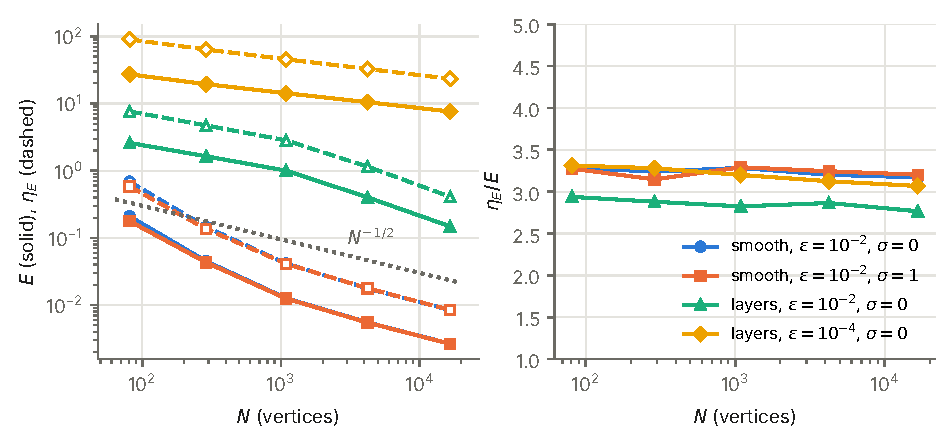
\includegraphics[width=\textwidth]{figures/sv_conv.pdf}
\caption{Uniform refinement in 2D, BJK. Left: $E$ (solid) and $\eta_E$ (dashed, open markers).
Right: effectivity index $I_E=\eta_E/E$.}
\label{fig:conv}
\end{figure}

\subsection{Robustness in \texorpdfstring{$\eps$}{eps}, \texorpdfstring{$\sigma$}{sigma} and the stabilisation}\label{sec:num-robust}

Table~\ref{tab:sweep} and Figure~\ref{fig:sweep} sweep $\eps$ from $10^{-1}$ to $10^{-8}$ on the fixed
mesh $n=32$, for $\sigma\in\{0,1\}$, both stabilisations and both problems.
\begin{itemize}
  \item \textbf{$\sigma=0$.} $I_E$ lies in $2.80$--$3.23$ for the layers problem and in $3.15$--$3.78$
  for the smooth problem, and becomes constant for $\eps\le10^{-5}$. $I_\oplus$ stays below $4.9$,
  and the stabilisation part is estimated sharply, $I_S=1.21$--$1.34$. BJK and SMUAS give the
  same indices $I_E$ and $I_\oplus$ to within $3\,\%$, as Remark~\ref{rem:robust} predicts: the limiter enters only
  through the functional, not the constants.
  \item \textbf{Energy norm.} The energy-norm index $I$ grows like $\eps^{-1}$ for $\sigma=0$, up to
  $2.5\cdot10^6$ at $\eps=10^{-8}$; the guaranteed energy-norm bound of \cite{ABR17} behaves in the
  same way. For $\sigma=1$, $I$ saturates at about $60$--$90$, the reaction giving $L^2$ control, while
  the ABR17 bound keeps growing ($1.3\cdot10^4$ at $\eps=10^{-8}$), because its reaction cut-off is not
  robust.
  \item \textbf{$\sigma=1$, small $\eps$.} Down to $\eps=10^{-6}$, $I_E$ stays in $2.7$--$3.2$ for the
  layers problem and in $3.2$--$4.9$ for the smooth one. For $\eps<10^{-6}$ it rises, to $5.5$ (layers)
  and $6.0$ (smooth) at $\eps=10^{-8}$. This increase comes from $I_S$ ($7.8$ and $10.4$ at
  $\eps=10^{-8}$), while $I_\oplus$ \emph{decreases}. This is consistent with a
  reference effect rather than with a loss of robustness: for $\sigma>0$, the Riesz representative of
  $\Stil$ has layers of width $(\eps/\sigma)^{1/2}=10^{-4}$, far below the mesh size $3\cdot10^{-2}$, so
  the same-mesh $P_2$ reference underestimates $\|\Stil\|_*$. Theorem~\ref{thm:eff} bounds $\eta_S$ by
  the true dual norm, independently of $\eps$. The adaptive runs of Section~\ref{sec:num-unad} confirm this:
  once the mesh resolves the layers, $I_S$ falls to $1.5$--$1.6$ and $I_E$ to about $3$.
\end{itemize}

% ---- begin tables/sweep.tex (inlined) ----
% generated by examples/convection_diffusion/sv_numerics/make_figures.py; do not edit
\begin{table}[!htbp]
\centering
\footnotesize
\setlength{\tabcolsep}{4pt}
\caption{Robustness in $\eps$ and $\sigma$ on the uniform mesh with $n=32$ ($N=1089$). $I_E=\eta_E/E$, $I_\oplus=\kappa\eta/\tnorm{e}_\oplus$, $I_S=\eta_S/\|\Stil\|_*$, $I=\eta/\tnorm{e}$ and, for comparison, the effectivity $I_{\mathrm{ABR17}}$ of the guaranteed energy-norm bound of \cite{ABR17}.}\label{tab:sweep}
\begin{tabular}{llrrrrrrrr}
\toprule
case & index & $10^{-1}$ & $10^{-2}$ & $10^{-3}$ & $10^{-4}$ & $10^{-5}$ & $10^{-6}$ & $10^{-7}$ & $10^{-8}$\\
\midrule
layers, BJK, $\sigma=0$ & $I_E$ & 2.96 & 2.82 & 3.06 & 3.20 & 3.23 & 3.23 & 3.23 & 3.23\\
 & $I_\oplus$ & 2.98 & 3.56 & 4.30 & 4.75 & 4.84 & 4.84 & 4.84 & 4.84\\
 & $I_S$ & 1.26 & 1.24 & 1.24 & 1.22 & 1.22 & 1.22 & 1.22 & 1.22\\
 & $I$ & 1.06 & 2.21 & 7.95 & 82.17 & $2.5\cdot10^{3}$ & $2.5\cdot10^{4}$ & $2.5\cdot10^{5}$ & $2.5\cdot10^{6}$\\
 & $I_{\mathrm{ABR17}}$ & 1.47 & 1.93 & 6.26 & 64.53 & $1.9\cdot10^{3}$ & $1.9\cdot10^{4}$ & $1.9\cdot10^{5}$ & $1.9\cdot10^{6}$\\
\addlinespace
layers, BJK, $\sigma=1$ & $I_E$ & 3.03 & 3.13 & 3.16 & 2.97 & 2.81 & 3.04 & 3.83 & 5.47\\
 & $I_\oplus$ & 3.05 & 3.95 & 4.25 & 4.02 & 3.83 & 3.50 & 3.28 & 3.24\\
 & $I_S$ & 1.29 & 1.29 & 1.41 & 1.54 & 1.66 & 2.55 & 4.41 & 7.79\\
 & $I$ & 1.09 & 2.33 & 6.39 & 30.27 & 74.58 & 71.78 & 67.57 & 66.77\\
 & $I_{\mathrm{ABR17}}$ & 1.47 & 1.94 & 6.25 & 57.80 & 391.31 & $1.3\cdot10^{3}$ & $4.0\cdot10^{3}$ & $1.3\cdot10^{4}$\\
\addlinespace
layers, SMUAS, $\sigma=0$ & $I_E$ & 2.95 & 2.80 & 3.01 & 3.15 & 3.17 & 3.18 & 3.18 & 3.18\\
 & $I_\oplus$ & 2.97 & 3.57 & 4.29 & 4.73 & 4.82 & 4.82 & 4.82 & 4.82\\
 & $I_S$ & 1.34 & 1.24 & 1.25 & 1.23 & 1.23 & 1.23 & 1.23 & 1.23\\
 & $I$ & 1.06 & 2.26 & 8.09 & 83.92 & $2.7\cdot10^{3}$ & $2.7\cdot10^{4}$ & $2.7\cdot10^{5}$ & $2.7\cdot10^{6}$\\
 & $I_{\mathrm{ABR17}}$ & 1.47 & 1.97 & 6.38 & 65.99 & $2.2\cdot10^{3}$ & $2.2\cdot10^{4}$ & $2.2\cdot10^{5}$ & $2.2\cdot10^{6}$\\
\addlinespace
layers, SMUAS, $\sigma=1$ & $I_E$ & 3.03 & 3.10 & 3.10 & 2.91 & 2.73 & 2.97 & 3.78 & 5.42\\
 & $I_\oplus$ & 3.04 & 3.95 & 4.20 & 4.00 & 3.81 & 3.49 & 3.27 & 3.24\\
 & $I_S$ & 1.37 & 1.28 & 1.41 & 1.50 & 1.61 & 2.46 & 4.26 & 7.53\\
 & $I$ & 1.08 & 2.36 & 6.14 & 28.08 & 66.99 & 64.21 & 60.54 & 59.85\\
 & $I_{\mathrm{ABR17}}$ & 1.47 & 1.99 & 6.38 & 58.84 & 389.93 & $1.3\cdot10^{3}$ & $4.0\cdot10^{3}$ & $1.3\cdot10^{4}$\\
\addlinespace
smooth, BJK, $\sigma=0$ & $I_E$ & 3.15 & 3.28 & 3.76 & 3.78 & 3.58 & 3.58 & 3.58 & 3.58\\
 & $I_\oplus$ & 3.17 & 3.46 & 4.85 & 4.49 & 3.87 & 3.86 & 3.85 & 3.85\\
 & $I_S$ & 1.29 & 1.30 & 1.24 & 1.21 & 1.22 & 1.22 & 1.22 & 1.22\\
 & $I$ & 1.12 & 1.31 & 6.28 & 77.92 & 778.23 & $6.9\cdot10^{3}$ & $6.8\cdot10^{4}$ & $6.8\cdot10^{5}$\\
 & $I_{\mathrm{ABR17}}$ & 1.70 & 1.76 & 5.18 & 74.26 & 842.71 & $7.5\cdot10^{3}$ & $7.4\cdot10^{4}$ & $7.4\cdot10^{5}$\\
\addlinespace
smooth, BJK, $\sigma=1$ & $I_E$ & 3.22 & 3.29 & 3.86 & 4.66 & 4.93 & 4.81 & 5.04 & 6.00\\
 & $I_\oplus$ & 3.24 & 3.46 & 4.82 & 5.50 & 5.68 & 5.22 & 4.79 & 4.69\\
 & $I_S$ & 1.32 & 1.37 & 1.45 & 1.66 & 2.24 & 3.41 & 5.88 & 10.39\\
 & $I$ & 1.14 & 1.29 & 5.60 & 42.08 & 90.00 & 92.63 & 85.82 & 84.22\\
 & $I_{\mathrm{ABR17}}$ & 1.70 & 1.76 & 5.05 & 49.08 & 229.66 & 763.28 & $2.4\cdot10^{3}$ & $7.7\cdot10^{3}$\\
\bottomrule
\end{tabular}
\end{table}
% ---- end tables/sweep.tex ----

\begin{figure}[!htbp]
\centering
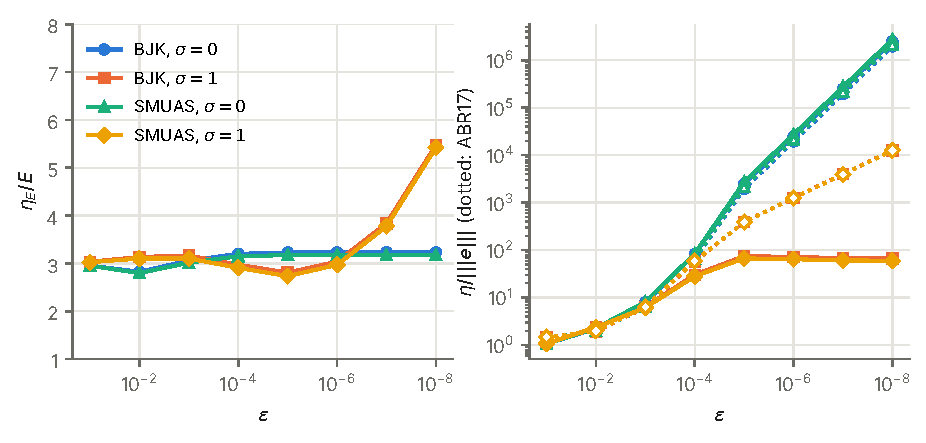
\includegraphics[width=\textwidth]{figures/sv_sweep.pdf}
\caption{Layers problem, $n=32$, as functions of $\eps$. Left: $I_E=\eta_E/E$. Right: the energy-norm
indices $\eta/\tnorm{e}$ (solid) and, dotted with open markers, that of the guaranteed bound of
\cite{ABR17}.}
\label{fig:sweep}
\end{figure}

\subsection{Variable reaction}\label{sec:num-cb}

With $c=1+(c_{\max}-1)xy$ and $\sigma=1$, the constant of (H3) is $\|c\|_\infty/\sigma=c_{\max}$, attained at
the vertex $(1,1)$. The computed $c_b$ is the sampled enclosure of Remark~\ref{rem:CF}, which is diagnostic: $c$ is not
affine on the cells, so the sampled maximum is enlarged by $\frac{h_K}2\max|\nabla c|$; here this gives $c_b=1.12\,c_{\max}$, $1.06\,c_{\max}$
and $1.03\,c_{\max}$ for $n=8,16,32$, and $\kappa=2+c_b$ (Table~\ref{tab:cb}). The bound $E\le\eta_E$ holds in
all runs. The index of $\eta_{E,c}$ grows at most linearly, $\eta_{E,c}/E_c\le3\,c_b$ in all runs, as
Corollary~\ref{cor:twoc} predicts; it is often much smaller, down to $0.05\,c_b$, because the factor $M=c_b$ in front of $\tnorm{e}$ in $E_c$ also enlarges the
error measure. The index of $\eta_E$ grows faster, up to $5.2\,c_b$ at $c_b\approx10^3$, but stays far
below the worst case $(1+c_b)^2$ of Corollary~\ref{cor:two}. A variable reaction with a small lower
bound $\sigma$ is therefore the one situation in which the estimator loses its robustness, in
accordance with the theory; Section~\ref{sec:concl} discusses how to remove it.

% ---- begin tables/cb.tex (inlined) ----
% generated by examples/convection_diffusion/sv_numerics/make_figures.py; do not edit
\begin{table}[!htbp]
\centering
\small
\setlength{\tabcolsep}{4pt}
\caption{Variable reaction $c=1+(c_{\max}-1)xy$, $\sigma=1$, $\eps\in\{10^{-3},10^{-6}\}$, $n\in\{8,16,32\}$: ranges over the six runs; $c_b$ and $\kappa$ are the means of the sampled enclosures (Remark~\ref{rem:CF}; diagnostic), which exceed $c_{\max}$ by $3$--$12\,\%$.}\label{tab:cb}
\begin{tabular}{rrrllll}
\toprule
$c_{\max}$ & $c_b$ & $\kappa$ & $\eta_E/E$ & $\eta_{E,c}/E_c$ & $\eta_{E,c}/(c_bE_c)$ & $E\le\eta_E$\\
\midrule
1 & 1.00 & 3.00 & 3.85--5.34 & 3.85--5.34 & 3.85--5.34 & yes\\
10 & 10.66 & 12.66 & 14.63--19.94 & 8.69--30.35 & 0.85--2.95 & yes\\
100 & 107.22 & 109.22 & 128--271 & 12.27--216 & 0.12--2.09 & yes\\
1000 & $1.1\cdot10^{3}$ & $1.1\cdot10^{3}$ & 1618--5312 & 56.23--1125 & 0.05--1.09 & yes\\
\bottomrule
\end{tabular}
\end{table}
% ---- end tables/cb.tex ----

\subsection{Local efficiency}\label{sec:num-loc}

Table~\ref{tab:loc} reports the localised measure for the layers problem on the $16\times16$ mesh. The
local ratio $\max_K\eta_K^2/E_{\mathrm{loc}}(\tilde\omega_K)^2$ is at most $0.51$ in all cases, and
independent of $\eps$ for $\eps\le10^{-4}$: the estimator is locally efficient, as stated in
Theorem~\ref{thm:loc}. The ratio $E_{\mathrm{loc}}/E$ lies between $0.48$ and $1.01$, so on these
problems the localised measure captures most of the global one, and the guaranteed bound
$E_{\mathrm{loc}}\le\sqrt{d+1}\,\eta_E$ of Theorem~\ref{thm:loc} overestimates $E_{\mathrm{loc}}$ by a
factor $5$--$12$. The largest value, $\eta_E/E_{\mathrm{loc}}=7.0$ for $\sigma=1$ and $\eps=10^{-8}$, is the
same reference effect as in Section~\ref{sec:num-robust}.

% ---- begin tables/loc.tex (inlined) ----
% generated by examples/convection_diffusion/sv_numerics/make_figures.py; do not edit
\begin{table}[!htbp]
\centering
\small
\setlength{\tabcolsep}{4pt}
\caption{Localised measure (Theorem~\ref{thm:loc}), outflow layers, BJK, $n=16$. The last but one column is $\max_K\eta_K^2/E_{\mathrm{loc}}(\tilde\omega_K)^2$ with $\eta_K=\eta_{A,K}+\eta_{S,K}$.}\label{tab:loc}
\begin{tabular}{rrrrrrr}
\toprule
$\sigma$ & $\eps$ & $E_{\mathrm{loc}}/E$ & $\eta_E/E_{\mathrm{loc}}$ & $\sqrt{d+1}\,\eta_E/E_{\mathrm{loc}}$ & local max & $I_E$\\
\midrule
0 & $10^{-2}$ & 0.48 & 5.94 & 10.29 & 0.26 & 2.88\\
0 & $10^{-4}$ & 0.60 & 5.50 & 9.53 & 0.37 & 3.28\\
0 & $10^{-6}$ & 0.60 & 5.50 & 9.52 & 0.37 & 3.29\\
0 & $10^{-8}$ & 0.60 & 5.50 & 9.52 & 0.37 & 3.29\\
1 & $10^{-2}$ & 0.52 & 6.38 & 11.05 & 0.51 & 3.33\\
1 & $10^{-4}$ & 0.95 & 3.07 & 5.32 & 0.13 & 2.93\\
1 & $10^{-6}$ & 1.01 & 3.47 & 6.01 & 0.07 & 3.51\\
1 & $10^{-8}$ & 1.01 & 7.04 & 12.20 & 0.07 & 7.13\\
\bottomrule
\end{tabular}
\end{table}
% ---- end tables/loc.tex ----

\subsection{Adaptive refinement}\label{sec:num-adapt}

Starting from the $8\times8$ mesh, we mark by the indicators $\eta_K=\eta_{A,K}+\eta_{S,K}$ with the
dual strategy of \cite{AJ27} (all cells with $\eta_K\ge\theta\max\eta$, $\theta=0.5$, reduced until at least
$5\,\%$ of the cells are marked) and refine by red--green refinement, until $N>3\cdot10^4$.
Table~\ref{tab:adapt} and Figures~\ref{fig:adapt} and~\ref{fig:adaptmesh} show the results for the layers
problem.
\begin{itemize}
  \item \textbf{Effectivity.} $I_E$ stays between $2.86$ and $3.55$ in every loop of all three runs, from
  $N=81$ to $N=45\,094$, while the local mesh size spans three orders of magnitude.
  \item \textbf{Where the mesh is refined.} The refinement concentrates in the outflow layers at $x=1$ and
  $y=1$ (Figure~\ref{fig:adaptmesh}); the smallest cells have $h_{\min}=3.5\cdot10^{-4}$ for $\eps=10^{-3}$,
  below $\eps$, so the layers are resolved, and $h_{\min}=1.7\cdot10^{-4}$ for $\eps=10^{-5}$, where they are not.
  \item \textbf{Convergence.} For $\eps=10^{-3}$, $E$ decreases at the rate $1.8$--$1.9$ with respect to
  $N^{-1/2}$ over the second half of the loops: this is the pre-asymptotic phase in which the layers become
  resolved, faster than the optimal rate $1$. For $\eps=10^{-5}$ the rate is $0.98$. On the finest uniform mesh
  ($N=16\,641$) the error $E$ is $18$, $4.4$ and $17$ times larger than the adaptive error at the same $N$.
  Under uniform refinement $E$ decreases at the rate $0.46$--$0.60$ for $\sigma=0$ and $0.04$--$0.51$ for
  $\sigma=1$, because the layers are never resolved; the index $I_E$ is $2.86$--$3.37$ there as well.
  \item \textbf{Energy norm.} Along the adaptive runs the energy-norm index $I$ falls from $29$ to $1.1$
  ($\eps=10^{-3}$) and from $8.4\cdot10^3$ to $6.2$ ($\eps=10^{-5}$): once the mesh resolves the layers, the
  energy error and the dual norm of the residual become comparable, while $I_E$ is insensitive to this.
\end{itemize}

% ---- begin tables/adapt.tex (inlined) ----
% generated by examples/convection_diffusion/sv_numerics/make_figures.py; do not edit
\begin{table}[!htbp]
\centering
\small
\setlength{\tabcolsep}{4pt}
\caption{Adaptive refinement for the outflow-layers problem, BJK, dual marking by the SV indicators $\eta_K$, red--green refinement. The rate is that of $E$ with respect to $N^{-1/2}$ over the second half of the loops; the last column is the ratio of $E$ on the finest uniform mesh ($N=16641$) to the adaptive $E$ at the same $N$.}\label{tab:adapt}
\begin{tabular}{rrrrllrlr}
\toprule
$\eps$ & $\sigma$ & loops & $N$ (last) & $h_{\min}$ & $E$ (last) & rate & $\eta_E/E$ & gain\\
\midrule
$10^{-3}$ & 0 & 15 & 33010 & $3.45\cdot10^{-4}$ & $7.395\cdot10^{-2}$ & 1.88 & 2.86--3.25 & 18.3\\
$10^{-5}$ & 0 & 12 & 31866 & $1.73\cdot10^{-4}$ & $3.941$ & 0.98 & 2.94--3.35 & 4.4\\
$10^{-3}$ & 1 & 17 & 45094 & $1.73\cdot10^{-4}$ & $5.891\cdot10^{-2}$ & 1.83 & 2.96--3.55 & 17.2\\
\bottomrule
\end{tabular}
\end{table}
% ---- end tables/adapt.tex ----

\begin{figure}[!htbp]
\centering
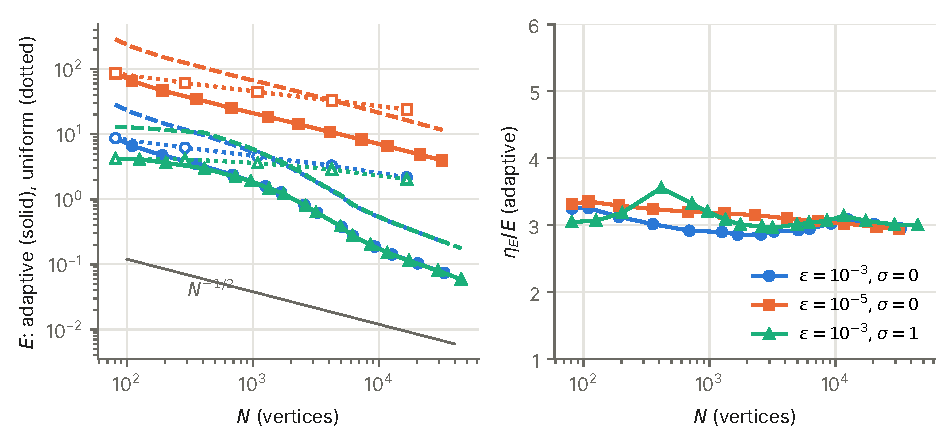
\includegraphics[width=\textwidth]{figures/sv_adapt.pdf}
\caption{Adaptive refinement, layers problem, BJK. Left: $E$ for adaptive (solid) and uniform (dotted, open
markers) refinement, and $\eta_E$ for the adaptive runs (dashed). Right: $I_E$ along the adaptive runs.}
\label{fig:adapt}
\end{figure}

\begin{figure}[!htbp]
\centering
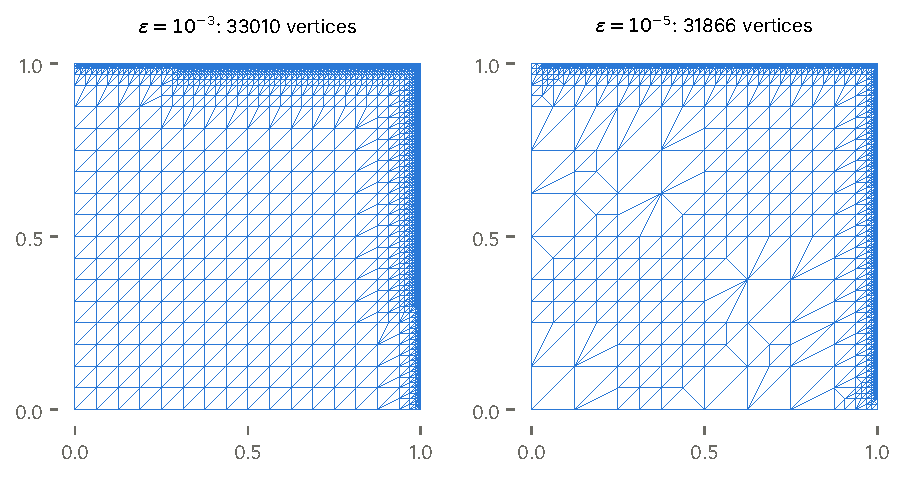
\includegraphics[width=\textwidth]{figures/sv_adapt_mesh.pdf}
\caption{Final adaptive meshes, layers problem, $\sigma=0$.}
\label{fig:adaptmesh}
\end{figure}

\subsection{Uniform versus adaptive refinement}\label{sec:num-unad}


We repeat the uniform-mesh studies of Tables~\ref{tab:conv} and~\ref{tab:sweep} with adaptive refinement:
the same problems, the same marking as in Section~\ref{sec:num-adapt}, from the $8\times8$ mesh up to
$N\approx2\cdot10^4$ (Table~\ref{tab:conv}) and $N\approx10^4$ (Table~\ref{tab:sweep}). For the robustness
sweep we compare at equal cost: the adaptive loop whose $N$ is closest to $N=1089$, the size of the $32\times32$
mesh of Table~\ref{tab:sweep}.

\paragraph{Refinement studies (Figure~\ref{fig:aconv}).}
\begin{itemize}
  \item \textbf{Effectivity.} Along the adaptive runs $I_E$ lies in $2.83$--$4.18$ and settles in the last
  loops at about $2.8$--$3.2$, close to the uniform values. The bound held in every loop.
  \item \textbf{Accuracy.} For the smooth solution, adaptive refinement gains nothing: at $N=16\,641$ the two
  errors agree to within $1\,\%$, and $E$ converges at the rate $1$ in both cases. For the layers problem the
  uniform error is $5.4$ ($\eps=10^{-2}$) and $5.9$ ($\eps=10^{-4}$) times the adaptive one at the same $N$.
  For $\eps=10^{-4}$, $E$ converges at the rate $0.47$ under uniform refinement and at $1.4$--$1.9$ in the last
  adaptive loops, in which the layers become resolved.
\end{itemize}

\begin{figure}[!htbp]
\centering
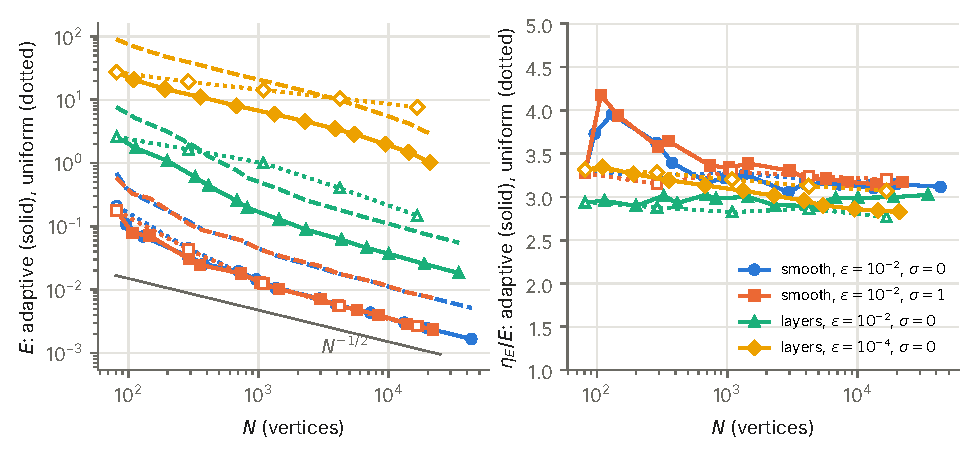
\includegraphics[width=\textwidth]{figures/sv_aconv.pdf}
\caption{The cases of Table~\ref{tab:conv} under adaptive refinement. Left: $E$ for adaptive (solid) and uniform
(dotted, open markers) refinement, and $\eta_E$ for the adaptive runs (dashed). Right: $I_E$, adaptive (solid) and
uniform (dotted).}
\label{fig:aconv}
\end{figure}

\paragraph{Robustness sweep (Figures~\ref{fig:abudget} and~\ref{fig:aloops}).}
\begin{itemize}
  \item \textbf{$\sigma=0$.} At equal cost, $I_E=2.89$--$3.22$ on the adaptive meshes against $2.80$--$3.23$ on the
  uniform mesh, for all $\eps$ and both stabilisations, and it stays in $2.82$--$3.35$ over all loops: the
  estimator is as robust on the meshes it generates as on the fixed mesh.
  \item \textbf{$\sigma=1$, small $\eps$.} The rise of $I_E$ to $5.4$--$5.5$ on the uniform mesh at
  $\eps\le10^{-7}$ (Section~\ref{sec:num-robust}) does not occur at equal cost on the adaptive meshes, where
  $I_E=2.75$--$3.16$. Figure~\ref{fig:aloops} shows why. The large values, up to $9.6$, appear only on the
  coarse initial mesh, and they come from the stabilisation part: $I_S=17.8$ at $N=81$ for $\eps=10^{-8}$. As the
  mesh resolves the layers, $I_S$ falls to $1.5$--$1.6$ and $I_E$ returns to about $3$. This confirms that the
  rise on the uniform mesh is a property of the under-resolved $P_2$ reference for $\|\Stil\|_*$, not of the
  estimator.
  \item \textbf{Smooth problem.} For $\eps\le10^{-3}$ the adaptive indices are higher than the uniform ones at
  equal cost: $I_E=4.0$--$5.3$ against $3.6$--$3.8$ for $\sigma=0$, and $4.5$--$6.0$ against $3.9$--$6.0$ for
  $\sigma=1$. Along the runs they reach $7.8$ after the first loop, and $10.9$ on the initial mesh. For $\sigma=1$
  and $\eps\le10^{-6}$ the fixed-point iteration reaches the iteration limit $2\cdot10^4$ on most meshes beyond
  $N\approx1100$, and the bound holds at these iterates.
  \item \textbf{Energy norm.} At $\sigma=0$ the energy-norm index still grows like $\eps^{-1}$ on the adaptive meshes,
  to $4\cdot10^5$ at $\eps=10^{-8}$ (uniform: $2.5\cdot10^6$); only the augmented measure is robust.
  \item \textbf{An open point.} For the layers problem with $\sigma=1$ and $\eps=10^{-6}$, $I_E$ rises again in the
  last loops, from $2.8$ to $4.3$, together with $I_\oplus$ (from $3.2$ to $6.6$). We have not identified the cause;
  it may be the convective part of the reference becoming resolved, and would need runs beyond $N=10^4$.
\end{itemize}

\begin{figure}[!htbp]
\centering
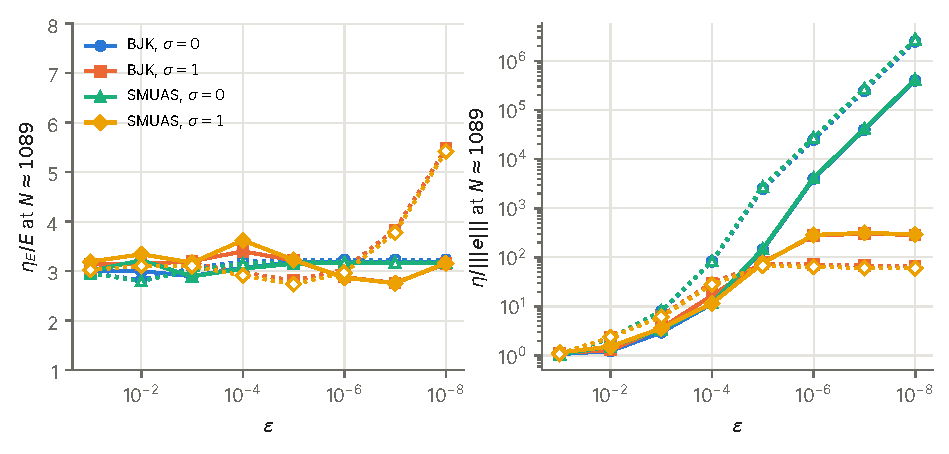
\includegraphics[width=\textwidth]{figures/sv_asweep_budget.pdf}
\caption{The robustness sweep of Table~\ref{tab:sweep} at equal cost, layers problem: adaptive meshes with
$N\approx1089$ (solid) against the uniform $32\times32$ mesh (dotted, open markers). Left: $I_E$. Right: the
energy-norm index $\eta/\tnorm{e}$.}
\label{fig:abudget}
\end{figure}

\begin{figure}[!htbp]
\centering
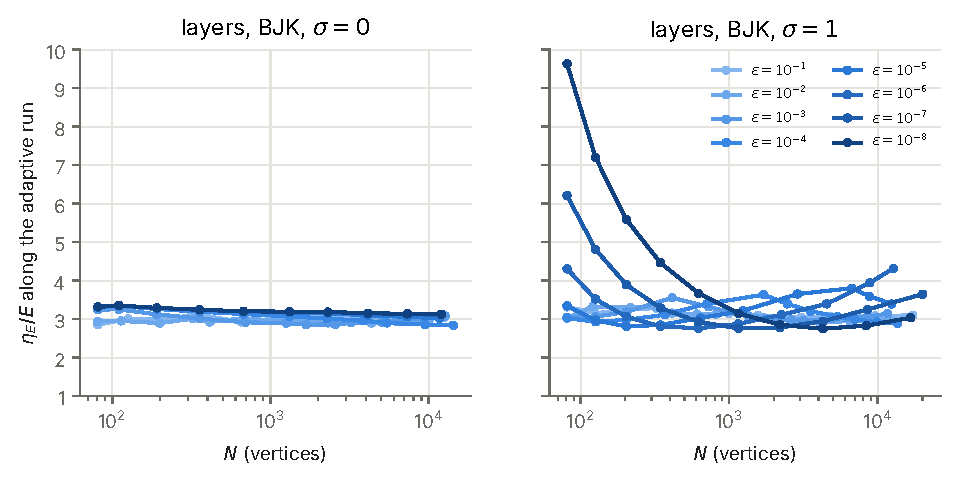
\includegraphics[width=\textwidth]{figures/sv_asweep_loops.pdf}
\caption{$I_E$ along the adaptive runs of the robustness sweep, layers problem, BJK; one line per $\eps$, darker for
smaller $\eps$.}
\label{fig:aloops}
\end{figure}

\paragraph{Which refinement to use.} For computing solutions, adaptive refinement is clearly preferable when the
solution has layers, by factors $4$--$18$ in $E$ at equal $N$, and it is what the estimator is designed for. For
testing the theory, the uniform meshes remain the primary evidence: a fixed coarse mesh keeps the layers
unresolved, which is the regime in which robustness can fail, isolates the dependence on $\eps$ and $\sigma$, and
is the only setting in which rates in $h$ are meaningful. The adaptive runs confirm that the effectivity stays at
about $3$ on the meshes the estimator generates itself.
% end of the magenta block

\subsection{Inexact iterates and adaptive stopping}\label{sec:num-stop}

\paragraph{Iterates.} Table~\ref{tab:iter} and Figure~\ref{fig:iter} evaluate the estimator at the
fixed-point iterates $u^i$ on the $16\times16$ mesh. The index $I_E$ stays between $2.9$ and $5.3$ at
every iterate, including the first one, where the algebraic part $\eta_{\mathrm{alg}}$ is up to $71\,\%$
of $\eta_{\mathrm{disc}}$: this is part~2 of Proposition~\ref{prop:stop}, efficiency at every iterate
without any condition on the algebraic error. The ratio $\eta_{\mathrm{alg}}/\eta_{\mathrm{disc}}$
decreases monotonically for all problems except the smooth one with $\eps=10^{-6}$ and $\sigma=0$, for
which the fixed-point iteration does not converge in $2\cdot10^4$ iterations; there the ratio stalls
at about $4\cdot10^{-3}$ for $i=200$--$1000$ and is $6\cdot10^{-4}$ at $i=2\cdot10^4$. In that case the error is smallest at $i\approx10$, $E(u^{10})=4.8$, and grows to
$8.4$ at $i=2\cdot10^4$: further iterations make the iterate worse in $E$, and the estimator, which is
efficient at every iterate, reflects this.

% ---- begin tables/iter.tex (inlined) ----
% generated by examples/convection_diffusion/sv_numerics/make_figures.py; do not edit
\begin{table}[!htbp]
\centering
\small
\setlength{\tabcolsep}{4pt}
\caption{Fixed-point iterates $u^i$, $i\in\{1,2,5,\dots,1000\}$ below the converged count, and the converged solution; BJK, $n=16$. The split is $\eta_{\mathrm{disc}}=\eta_E-\eta_{\mathrm{alg}}$.}\label{tab:iter}
\begin{tabular}{lrrrlrrl}
\toprule
problem & $\eps$ & $\sigma$ & it.\ to tol. & $\eta_E/E$ over $i$ & $\max_i\eta_{\mathrm{alg}}/\eta_{\mathrm{disc}}$ & $E(u^1)/E(u^{\mathrm{last}})$ & $E\le\eta_E$\\
\midrule
smooth & $10^{-2}$ & 0 & 39 & 3.24--3.63 & 0.71 & 1.81 & yes\\
smooth & $10^{-2}$ & 1 & 37 & 3.15--3.45 & 0.51 & 1.58 & yes\\
smooth & $10^{-6}$ & 0 & 20000 & 3.76--4.61 & 0.58 & 1.06 & yes\\
smooth & $10^{-6}$ & 1 & 664 & 4.42--5.28 & 0.19 & 1.20 & yes\\
layers & $10^{-2}$ & 0 & 47 & 2.88--2.97 & 0.02 & 1.01 & yes\\
layers & $10^{-2}$ & 1 & 45 & 3.32--3.33 & 0.01 & 1.01 & yes\\
layers & $10^{-6}$ & 0 & 635 & 3.29--3.47 & 0.04 & 1.01 & yes\\
layers & $10^{-6}$ & 1 & 502 & 3.51--3.56 & 0.02 & 1.03 & yes\\
\bottomrule
\end{tabular}
\end{table}
% ---- end tables/iter.tex ----

\begin{figure}[!htbp]
\centering
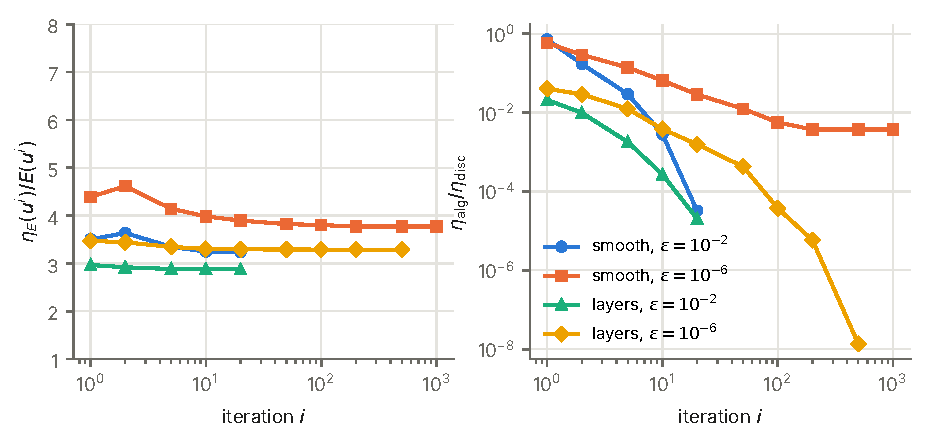
\includegraphics[width=\textwidth]{figures/sv_iter.pdf}
\caption{Fixed-point iterates, BJK, $\sigma=0$, $n=16$. Left: $I_E$ at the iterate $u^i$. Right: the
ratio $\eta_{\mathrm{alg}}/\eta_{\mathrm{disc}}$ (points with a ratio below $10^{-8}$ are omitted).}
\label{fig:iter}
\end{figure}

\paragraph{Adaptive stopping.} Table~\ref{tab:stop} runs five adaptive loops as in Section~\ref{sec:num-adapt}
in which the fixed-point iteration is stopped either at the fixed tolerance $\|r\|\le10^{-10}\sqrt N$ or by
the criterion \eqref{eq:stop}, $\eta_{\mathrm{alg}}\le\gamma\eta_{\mathrm{disc}}$, with
$\eta_{\mathrm{disc}}=\eta_E-\eta_{\mathrm{alg}}$; each loop starts from the zero initial guess.
\begin{itemize}
  \item \textbf{Savings.} With $\gamma=0.1$, the total number of iterations drops from $227$ to $25$ (smooth,
  $\eps=10^{-2}$) and from $2323$ to $25$ (layers, $\eps=10^{-4}$), by factors $9$ and $93$; with $\gamma=0.01$
  the factors are $4.5$ and $46$.
  \item \textbf{Accuracy.} The final error $E$ changes by at most $6\,\%$ ($\gamma=0.1$, layers) and by at most
  $0.3\,\%$ for $\gamma\le0.01$. The index $I_E$ stays in $3.1$--$4.8$ in all runs, and in every stopped loop
  $\eta_{\mathrm{alg}}/\eta_{\mathrm{disc}}\le\gamma$, so $E\le(1+\gamma)\eta_{\mathrm{disc}}$
  (Proposition~\ref{prop:stop}, part~3).
  \item \textbf{Non-converging iteration.} For the smooth problem with $\eps=10^{-6}$ the fixed-point
  iteration does not reach the tolerance within $10^4$ iterations on any mesh, and $50\,000$ iterations give
  $E=3.22$. The criterion with $\gamma=0.1$ stops after $5$--$15$ iterations per loop, $50$ in total, with a
  \emph{smaller} error, $E=1.98$: as in Figure~\ref{fig:iter}, the early iterates are better than the late
  ones. For $\gamma=10^{-3}$ the criterion fires in only one of the five loops, since $\eta_{\mathrm{alg}}/\eta_{\mathrm{disc}}$ stalls
  at about $3\cdot10^{-3}$; this is a property of the iteration, not of the estimator.
\end{itemize}

% ---- begin tables/stop.tex (inlined) ----
% generated by examples/convection_diffusion/sv_numerics/make_figures.py; do not edit
\begin{table}[!htbp]
\centering
\footnotesize
\setlength{\tabcolsep}{4pt}
\caption{Adaptive stopping in five adaptive loops (dual marking by the SV indicators, red--green refinement), BJK, $\sigma=0$. ``tol.'' is the fixed tolerance $\|r\|\le10^{-10}\sqrt N$; otherwise the iteration stops at $\eta_{\mathrm{alg}}\le\gamma\eta_{\mathrm{disc}}$ (at most $10^4$ iterations). The last column says whether every loop stopped before the iteration limit.}\label{tab:stop}
\begin{tabular}{lrrrrlllr}
\toprule
problem & $\eps$ & $\gamma$ & it./loop & total & $E$ (last) & $\eta_E/E$ & $\max\eta_{\mathrm{alg}}/\eta_{\mathrm{disc}}$ & stopped\\
\midrule
smooth & $10^{-2}$ & tol. & 30--59 & 227 & $2.550\cdot10^{-2}$ & 3.29--3.95 & $5.78\cdot10^{-8}$ & yes\\
smooth & $10^{-2}$ & 0.1 & 5 & 25 & $2.554\cdot10^{-2}$ & 3.41--3.97 & $5.07\cdot10^{-2}$ & yes\\
smooth & $10^{-2}$ & 0.01 & 10 & 50 & $2.551\cdot10^{-2}$ & 3.33--3.98 & $7.27\cdot10^{-3}$ & yes\\
smooth & $10^{-2}$ & 0.001 & 10--20 & 80 & $2.551\cdot10^{-2}$ & 3.29--3.96 & $9.89\cdot10^{-4}$ & yes\\
smooth & $10^{-6}$ & tol. & 10000 & 50000 & $3.218$ & 3.77--4.58 & $3.03\cdot10^{-3}$ & no\\
smooth & $10^{-6}$ & 0.1 & 5--15 & 50 & $1.984$ & 4.04--4.79 & $9.83\cdot10^{-2}$ & yes\\
smooth & $10^{-6}$ & 0.01 & 120--760 & 2190 & $2.749$ & 3.80--4.45 & $9.10\cdot10^{-3}$ & yes\\
smooth & $10^{-6}$ & 0.001 & 7320--10000 & 47320 & $3.218$ & 3.77--4.58 & $3.03\cdot10^{-3}$ & no\\
layers & $10^{-4}$ & tol. & 385--628 & 2323 & $8.044$ & 3.13--3.34 & $3.57\cdot10^{-9}$ & yes\\
layers & $10^{-4}$ & 0.1 & 5 & 25 & $8.524$ & 3.20--3.42 & $2.49\cdot10^{-2}$ & yes\\
layers & $10^{-4}$ & 0.01 & 10 & 50 & $8.023$ & 3.15--3.38 & $8.43\cdot10^{-3}$ & yes\\
layers & $10^{-4}$ & 0.001 & 25--50 & 175 & $8.04$ & 3.14--3.35 & $9.29\cdot10^{-4}$ & yes\\
\bottomrule
\end{tabular}
\end{table}
% ---- end tables/stop.tex ----

\subsection{Variable diffusion}\label{sec:num-vareps}

Table~\ref{tab:vareps} reports the variable-diffusion problems on the meshes $n=8,16,32$. All bounds are
guaranteed. For the smooth coefficient, the oscillation $\eta_\eps$ converges at the rate $2.09$--$2.13$
with respect to $N^{-1/2}$ ($2.00$--$2.04$ in $h$), in accordance with Lemma~\ref{lem:V}(iii), and is at most $12\,\%$ of $\eta$ (at contrast $10^4$ on
the coarsest mesh). For the jump aligned with the mesh, $\Pi_1\eps=\eps$ and $\eta_\eps=0$. The
effectivity $I_E$ lies in $2.6$--$4.5$ for contrasts up to $10^4$, for $\eps=10^{-2}$ and $10^{-6}$ alike. For
the jump it does not grow with the contrast; for the smooth coefficient it grows mildly, from
$3.1$--$3.7$ at contrast $1$ to at most $4.3$ ($\eps=10^{-2}$) and $4.5$ ($\eps=10^{-6}$) at contrast $10^4$, both
on the coarsest mesh. This is the quasi-monotone case; the constants of
Theorem~\ref{thm:vareps} depend on the patch contrast, but for an aligned jump that contrast does not
show up in the indices. Checkerboard (non-quasi-monotone) coefficients are not tested; for them no
local estimator can be robust \cite{Li26}.

% ---- begin tables/vareps.tex (inlined) ----
% generated by examples/convection_diffusion/sv_numerics/make_figures.py; do not edit
\begin{table}[!htbp]
\centering
\footnotesize
\setlength{\tabcolsep}{4pt}
\caption{Variable diffusion, BJK, $\sigma=0$, $n\in\{8,16,32\}$: ranges over the three meshes. The rate is that of $\eta_\eps$ with respect to $N^{-1/2}$ between $n=16$ and $n=32$ (expected: $2$).}\label{tab:vareps}
\begin{tabular}{lrrllllrl}
\toprule
$\eps(x)$ & $\eps$ & contrast & $I$ & $I_\oplus$ & $I_E$ & $\max\eta_\eps/\eta$ & rate & $E\le\eta_E$\\
\midrule
smooth & $10^{-2}$ & 1 & 1.23--4.58 & 3.30--4.06 & 3.07--3.13 & 0.000 & --- & yes\\
smooth & $10^{-2}$ & 100 & 1.07--1.24 & 3.16--3.39 & 3.15--3.26 & 0.035 & 2.09 & yes\\
smooth & $10^{-2}$ & 10000 & 1.10--1.44 & 3.30--4.28 & 3.29--4.27 & 0.117 & 2.09 & yes\\
smooth & $10^{-6}$ & 1 & 7959--36796 & 3.72--5.01 & 3.50--3.70 & 0.000 & --- & yes\\
smooth & $10^{-6}$ & 100 & 818--3354 & 3.73--5.44 & 3.54--4.03 & 0.000 & 2.13 & yes\\
smooth & $10^{-6}$ & 10000 & 64.07--336 & 4.31--5.49 & 3.94--4.46 & 0.001 & 2.10 & yes\\
jump & $10^{-2}$ & 100 & 2.56--7.63 & 3.43--4.18 & 2.61--2.99 & 0.000 & --- & yes\\
jump & $10^{-2}$ & 10000 & 2.61--8.12 & 3.43--4.22 & 2.60--3.01 & 0.000 & --- & yes\\
jump & $10^{-6}$ & 100 & 9025--28125 & 4.75--5.12 & 3.44--3.54 & 0.000 & --- & yes\\
jump & $10^{-6}$ & 10000 & 2156--4989 & 4.78--5.08 & 3.41--3.52 & 0.000 & --- & yes\\
\bottomrule
\end{tabular}
\end{table}
% ---- end tables/vareps.tex ----

\subsection{Three dimensions}\label{sec:num-3d}

Table~\ref{tab:d3} repeats the uniform-refinement study on the unit cube ($n=4,8,16$, up to $N=4913$
vertices and $24\,576$ tetrahedra).
\begin{itemize}
  \item \textbf{Layers.} $I_E=2.94$--$3.55$ for $\eps=10^{-2}$ and $10^{-6}$, as in two dimensions; $I_\oplus\le4.9$
  and $I_S=1.21$--$1.26$.
  \item \textbf{Smooth solution.} $I_E$ is higher than in two dimensions, $5.1$--$6.4$, but decreases under
  refinement for both values of $\eps$ ($5.97\to5.40$ and $6.39\to5.09$). These meshes are coarse: $E$ still
  converges at the pre-asymptotic rates $2.1$--$2.7$ in $h$, dominated by the stabilisation part
  $\|\Stil\|_*$, which is estimated sharply ($I_S=1.28$--$1.31$); the larger index comes from the convective
  dual norm on coarse tetrahedral meshes. For $\eps=10^{-6}$ on the finest mesh the fixed-point iteration does
  not converge within $2\cdot10^4$ iterations, and the bound still holds at the last iterate.
  \item \textbf{Energy norm.} As in two dimensions, $I$ is useless for $\sigma=0$ and small $\eps$
  ($1.0\cdot10^4$--$1.4\cdot10^5$ at $\eps=10^{-6}$, against $2.6$--$9.3$ at $\eps=10^{-2}$), while $I_E$ is not
  affected.
  \item \textbf{Cost.} The estimator takes about $8$\,s at $N=729$ and $220$--$240$\,s at $N=4913$ in our
  Python implementation; the cost is dominated by the vertex-patch problems in $\RTN$, whose size grows
  quickly with the number of tetrahedra per patch in three dimensions. The patch problems are independent and
  can be solved in parallel; the global $\RT_0$ defect problem takes a small fraction of the time.
\end{itemize}

% ---- begin tables/d3.tex (inlined) ----
% generated by examples/convection_diffusion/sv_numerics/make_figures.py; do not edit
\begin{table}[!htbp]
\centering
\small
\setlength{\tabcolsep}{4pt}
\caption{Three dimensions, uniform refinement of the unit cube, BJK, $\sigma=0$. Rates with respect to $N^{-1/3}\sim h$; the last column is the time of the estimator in seconds.}\label{tab:d3}
\begin{tabular}{lrrlrrrrr}
\toprule
problem & $\eps$ & $N$ & $E$ & rate & $I$ & $I_\oplus$ & $I_E$ & time\\
\midrule
smooth & $10^{-2}$ & 125 & $0.7$ &  & 9.27 & 7.82 & 5.97 & 0.7\\
smooth & $10^{-2}$ & 729 & $0.144$ & 2.69 & 4.83 & 6.98 & 5.71 & 9.0\\
smooth & $10^{-2}$ & 4913 & $3.55\cdot10^{-2}$ & 2.20 & 2.64 & 5.84 & 5.40 & 226.6\\
smooth & $10^{-6}$ & 125 & $6.72\cdot10^{1}$ &  & $7.4\cdot10^{4}$ & 9.26 & 6.39 & 0.6\\
smooth & $10^{-6}$ & 729 & $2.00\cdot10^{1}$ & 2.06 & $2.8\cdot10^{4}$ & 6.93 & 5.31 & 8.4\\
smooth & $10^{-6}$ & 4913 & $4.06$ & 2.51 & $1.0\cdot10^{4}$ & 5.56 & 5.09 & 238.0\\
layers & $10^{-2}$ & 125 & $2.74$ &  & 6.67 & 4.01 & 3.10 & 0.6\\
layers & $10^{-2}$ & 729 & $1.82$ & 0.70 & 4.31 & 3.71 & 3.01 & 8.0\\
layers & $10^{-2}$ & 4913 & $1.14$ & 0.73 & 2.93 & 3.64 & 2.94 & 217.3\\
layers & $10^{-6}$ & 125 & $2.79\cdot10^{2}$ &  & $1.4\cdot10^{5}$ & 4.71 & 3.38 & 0.5\\
layers & $10^{-6}$ & 729 & $2.01\cdot10^{2}$ & 0.56 & $7.3\cdot10^{4}$ & 4.78 & 3.47 & 8.5\\
layers & $10^{-6}$ & 4913 & $1.35\cdot10^{2}$ & 0.63 & $3.8\cdot10^{4}$ & 4.93 & 3.55 & 236.1\\
\bottomrule
\end{tabular}
\end{table}
% ---- end tables/d3.tex ----

\subsection{Summary}

The experiments answer the questions (Q1)--(Q7) as follows.
\begin{enumerate}[label=(Q\arabic*)]
  \item The bound $E\le\eta_E$ held in every run: two and three dimensions, both stabilisations,
  $\eps=10^{-1},\dots,10^{-8}$, $\sigma\in\{0,1\}$, variable reaction and diffusion, adaptive meshes and inexact
  iterates, and so did $I\ge1$, $I_\oplus\ge1$ and $I_S\ge1$. Since the references are lower bounds of the dual
  norms, this is a consistency check rather than a proof.
  \item For constant coefficients, $I_E$ lies in $2.7$--$5.3$ in two dimensions, inexact iterates included,
  independently of $\eps$, $\sigma$, the stabilisation and the mesh; the only exception is a rise to $5.4$--$6.0$
  ($n=32$) and $7.1$ ($n=16$) at $\sigma=1$, $\eps\le10^{-7}$, which the adaptive runs identify as an
  under-resolved reference for $\|\Stil\|_*$ (Section~\ref{sec:num-unad}); in three dimensions it is $2.9$--$6.4$ and
  decreases under refinement. The energy-norm index $I$, and the guaranteed bound of \cite{ABR17}, are not
  robust.
  \item The effectivity grows with $c_b$, at most linearly for $\eta_{E,c}$ and well below $c_b^2$ for $\eta_E$:
  a variable reaction with a small lower bound is the one case in which robustness is lost, as the theory
  predicts.
  \item The local ratio $\max_K\eta_K^2/E_{\mathrm{loc}}(\tilde\omega_K)^2$ is at most $0.51$.
  \item Adaptive refinement driven by $\eta_K$ resolves the layers and reduces $E$ by factors $4$--$18$
  against uniform refinement at equal $N$, with $I_E=2.9$--$3.6$ throughout. Repeating the refinement and
  robustness studies adaptively gives the same effectivity, about $3$, as on uniform meshes.
  \item The estimator is efficient at every iterate, and the stopping criterion saves up to $99\,\%$ of the
  iterations at a change of the error of at most $6\,\%$ ($\gamma=0.1$) or $0.3\,\%$ ($\gamma\le0.01$).
  \item For variable diffusion, $\eta_\eps$ converges at rate $2$ and $I_E$ stays in $2.6$--$4.5$ up to contrast
  $10^4$.
\end{enumerate}

\paragraph{Reproducibility.} All results are produced by three scripts in the following directory of
\texttt{galerkit}:
\begin{center}
  \path{examples/convection_diffusion/sv_numerics}
\end{center}
\begin{itemize}
  \item \texttt{run\_numerics.py} runs the experiments (about $35$ minutes on four cores, the
  three-dimensional runs sequentially because of their memory use);
  \item \texttt{make\_figures.py} writes the tables, the figures and, for every stored solution, a VTK
  file (\texttt{.vtu}) with $u_h$, $u$, $u-u_h$, $\eps$, $\eta_K$, $\tnorm{e}_K$ and the local
  effectivity $\eta_K/\tnorm{e}_K$;
  \item \texttt{make\_adaptive\_figures.py} produces the figures of Section~\ref{sec:num-unad}.
\end{itemize}
% ---- end numeric.tex ----

% ===========================================================================
\section{Conclusions and open problems}\label{sec:concl}
% ===========================================================================

We have shown that the Smears--Vohral\'ik-type equilibrated-flux estimator, extended to convection
with the stabilisation as an additional diffusion tensor, is guaranteed and robustly locally
efficient for algebraically stabilised convection--diffusion--reaction problems. The proof needs no
weights in the patch problems and no use of the discrete equation, so it covers inexact iterates and
yields a stopping criterion without smallness conditions. Several questions remain open.
\begin{itemize}
  \item \textbf{Removing $c_b$.} The factors $(1+c_b)^2$ and $1+c_b$, the restriction of
  Theorem~\ref{thm:loc} to $\sigma>0$ or $c=\frac12\dv b$, and the additional term of
  Remark~\ref{rem:locfr} all stem from measuring the reaction by its lower bound $\sigma$. An energy
  norm with the full effective reaction $c-\frac12\dv b$, with cellwise weights in the spirit of
  \cite{AV14}, would remove all three.
  \item \textbf{Non-$P_1$ Dirichlet data.} The efficiency of the Dirichlet lifting terms is not
  treated.
  \item \textbf{Robustness in the diffusion contrast} is shown only numerically, and only for
  quasi-monotone $\eps$.
  \item \textbf{The stopped iterate against the discrete solution}, $E(u^i)\lesssim E(u_h)$, needs a
  discrete stability estimate for the nonlinear operator.
  \item \textbf{The direct variant} (Remark~\ref{rem:direct}) has no efficiency result.
\end{itemize}

% ===========================================================================
\begin{thebibliography}{PRVW20}
% ===========================================================================

\bibitem[ABR17]{ABR17}
A.~Allendes, G.~R.~Barrenechea, R.~Rankin,
Fully computable error estimation of a nonlinear, positivity-preserving discretization of the
convection--diffusion--reaction equation,
SIAM J.\ Sci.\ Comput.\ 39 (2017) A1903--A1927.

\bibitem[AJ27]{AJ27}
N.~Ahmed, A.~Jha,
Adaptive finite elements with algebraic stabilization for convection-dominated transport,
preprint, arXiv:2602.14504 (2026).

\bibitem[AV11]{AV11}
M.~Ainsworth, T.~Vejchodsk\'y,
Fully computable robust a posteriori error bounds for singularly perturbed reaction--diffusion
problems,
Numer.\ Math.\ 119 (2011) 219--243.

\bibitem[AV14]{AV14}
M.~Ainsworth, T.~Vejchodsk\'y,
Robust error bounds for finite element approximation of reaction--diffusion problems with
non-constant reaction coefficient in arbitrary space dimension,
Comput.\ Methods Appl.\ Mech.\ Engrg.\ 281 (2014) 184--199.

\bibitem[BBK17]{BBK17}
G.~R.~Barrenechea, E.~Burman, F.~Karakatsani,
Edge-based nonlinear diffusion for finite element approximations of convection--diffusion equations
and its relation to algebraic flux-correction schemes,
Numer.\ Math.\ 135 (2017) 521--545.

\bibitem[BJK16]{BJK16}
G.~R.~Barrenechea, V.~John, P.~Knobloch,
Analysis of algebraic flux correction schemes,
SIAM J.\ Numer.\ Anal.\ 54 (2016) 2427--2451.

\bibitem[BJK17]{BJK17}
G.~R.~Barrenechea, V.~John, P.~Knobloch,
An algebraic flux correction scheme satisfying the discrete maximum principle and linearity
preservation on general meshes,
Math.\ Models Methods Appl.\ Sci.\ 27 (2017) 525--548.

\bibitem[BMV20]{BMV}
J.~Blechta, J.~M\'alek, M.~Vohral\'ik,
Localization of the $W^{-1,q}$ norm for local a posteriori efficiency,
IMA J.\ Numer.\ Anal.\ 40 (2020) 914--950.

\bibitem[BV00]{BV00}
C.~Bernardi, R.~Verfürth,
Adaptive finite element methods for elliptic equations with non-smooth coefficients,
Numer.\ Math.\ 85 (2000) 579--608.

\bibitem[CC25]{CC25}
D.~Cai, Z.~Cai,
Hybrid a posteriori error estimators for conforming finite element approximations to stationary
convection--diffusion--reaction equations,
Numer.\ Math.\ 157 (2025) 477--504.

\bibitem[CCZ]{CCZ}
C.~He, Z.~Cai, S.~Zhang,
Generalized Prager--Synge inequality and equilibrated error estimators for discontinuous elements,
preprint, arXiv:2001.09102 (2020).

\bibitem[CFPV09]{CFPV09}
I.~Cheddadi, R.~Fu\v{c}\'ik, M.~I.~Prieto, M.~Vohral\'ik,
Guaranteed and robust a posteriori error estimates for singularly perturbed reaction--diffusion
problems,
ESAIM Math.\ Model.\ Numer.\ Anal.\ 43 (2009) 867--888.

\bibitem[CHZ]{CHZ}
Z.~Cai, C.~He, S.~Zhang,
Residual-based a posteriori error estimate for interface problems: nonconforming linear elements,
preprint, arXiv:1603.01024 (2016).

\bibitem[CV18]{CV18}
P.~Ciarlet~Jr., M.~Vohral\'ik,
Localization of global norms and robust a posteriori error control for transmission problems with
sign-changing coefficients,
ESAIM Math.\ Model.\ Numer.\ Anal.\ 52 (2018) 2037--2064.

\bibitem[CW08]{CW08}
S.~H.~Christiansen, R.~Winther,
Smoothed projections in finite element exterior calculus,
Math.\ Comp.\ 77 (2008) 813--829.

\bibitem[DEV13]{DEV13}
V.~Dolej\v{s}\'i, A.~Ern, M.~Vohral\'ik,
A framework for robust a posteriori error control in unsteady nonlinear advection--diffusion problems,
SIAM J.\ Numer.\ Anal.\ 51 (2013) 773--793.

\bibitem[EM16]{EM16}
M.~Eigel, C.~Merdon,
Equilibration a posteriori error estimation for convection--diffusion--reaction problems,
J.\ Sci.\ Comput.\ 67 (2016) 747--768.

\bibitem[ESV10]{ESV10}
A.~Ern, A.~F.~Stephansen, M.~Vohral\'ik,
Guaranteed and robust discontinuous Galerkin a posteriori error estimates for
convection--diffusion--reaction problems,
J.\ Comput.\ Appl.\ Math.\ 234 (2010) 114--130.

\bibitem[EV13]{EV13}
A.~Ern, M.~Vohral\'ik,
Adaptive inexact Newton methods with a posteriori stopping criteria for nonlinear diffusion PDEs,
SIAM J.\ Sci.\ Comput.\ 35 (2013) A1761--A1791.

\bibitem[EV15]{EV15}
A.~Ern, M.~Vohral\'ik,
Polynomial-degree-robust a posteriori estimates in a unified setting for conforming, nonconforming,
discontinuous Galerkin, and mixed discretizations,
SIAM J.\ Numer.\ Anal.\ 53 (2015) 1058--1081.

\bibitem[HPSV21]{HPSV21}
A.~Haberl, D.~Praetorius, S.~Schimanko, M.~Vohral\'ik,
Convergence and quasi-optimal cost of adaptive algorithms for nonlinear operators including
iterative linearization and algebraic solver,
Numer.\ Math.\ 147 (2021) 679--725.

\bibitem[J21]{J21}
A.~Jha,
A residual based a posteriori error estimators for AFC schemes for convection-diffusion equations,
Comput.\ Math.\ Appl.\ 97 (2021) 86--99.

\bibitem[J24]{J24}
A.~Jha,
Residual-based a posteriori error estimators for algebraic stabilizations,
Appl.\ Math.\ Lett.\ 157 (2024) 109192.

\bibitem[Kn23]{Kn23}
P.~Knobloch,
An algebraically stabilized method for convection--diffusion--reaction problems with optimal
experimental convergence rates on general meshes,
Numer.\ Algorithms 94 (2023).

\bibitem[LDG20]{LDG20}
A.~Abdulle, G.~Rosilho de Souza,
A posteriori error analysis of a local adaptive discontinuous Galerkin method for
convection--diffusion--reaction equations,
J.\ Comput.\ Phys.\ 452 (2022) 110894; arXiv:2004.07148.

\bibitem[Li26]{Li26}
Y.~Li,
Locally computable error estimators for conforming approximations of interface problems cannot be
robust, preprint, arXiv:2609.27817 (2026).

\bibitem[Licht19]{Licht19}
M.~W.~Licht,
Smoothed projections and mixed boundary conditions,
Math.\ Comp.\ 88 (2019) 607--635.

\bibitem[Pe02]{Pe02}
M.~Petzoldt,
A posteriori error estimators for elliptic equations with discontinuous coefficients,
Adv.\ Comput.\ Math.\ 16 (2002) 47--75.

\bibitem[PRVW20]{PRVW20}
J.~Pap\v{e}z, U.~R\"ude, M.~Vohral\'ik, B.~Wohlmuth,
Sharp algebraic and total a posteriori error bounds for $h$ and $p$ finite elements via a multilevel
approach. Recovering mass balance in any situation,
Comput.\ Methods Appl.\ Mech.\ Engrg.\ 371 (2020) 113243.

\bibitem[Sa08]{Sa08}
G.~Sangalli,
Robust a-posteriori estimator for advection--diffusion--reaction problems,
Math.\ Comp.\ 77 (2008) 41--70.

\bibitem[SV20]{SV20}
I.~Smears, M.~Vohral\'ik,
Simple and robust equilibrated flux a posteriori estimates for singularly perturbed
reaction--diffusion problems,
ESAIM Math.\ Model.\ Numer.\ Anal.\ 54 (2020) 1951--1973.

\bibitem[TV15]{TV15}
L.~Tobiska, R.~Verfürth,
Robust a posteriori error estimates for stabilized finite element methods,
IMA J.\ Numer.\ Anal.\ 35 (2015) 1652--1671.

\bibitem[V05]{V05}
R.~Verfürth,
Robust a posteriori error estimates for stationary convection--diffusion equations,
SIAM J.\ Numer.\ Anal.\ 43 (2005) 1766--1782.

\end{thebibliography}

\end{document}
